\documentclass[a4paper]{book-enhanced}

\usepackage{src/preambolo}

% TODO GENERALI
% rifare in modo pulito tutte le figure pesantemente basate su coordinate
% rimuovere label inutili
% valutare se passare al semplice ref piuttosto che cref
% decidere se usare tuple (e nel caso farlo) per grafi e altri

\title{Algoritmi e Complessità}
\subtitle{Appunti delle lezioni tenute dal Prof. Paolo Boldi}
\author{Alessandro Clerici, Marco Cutecchia, Edoardo Marangoni}
\university{Università degli Studi di Milano}
\dept{Dipartimento di Informatica}
\logo{img/logo.tikz}

\begin{document}

\frontmatter

\maketitle
\tableofcontents

\mainmatter

\section*{Notazione}
\addcontentsline{toc}{section}{Notazione}


\subsection*{Insiemi}
Indicheremo la cardinalità di un insieme $A$ con $\card{A}$.
Indichiamo con $\N$ l'insieme dei numeri naturali, con $\Z$ i numeri interi (relativi), con $\Q$ i razionali e con $\R$ i reali.
Indichiamo con $S^+$, dove $S$ è uno degli insiemi sopracitati, il sottoinsieme dei numeri positivi di $S$.


\subsection*{Parole e linguaggi}
Se $\Sigma$ è un alfabeto (un insieme di simboli), sia $(\Sigma\star, \cdot, \emptyword)$ il monoide libero\footnote{Per un'introduzione alla relazione tra strutture algebriche e linguaggi (e la loro	chiusura di Kleene), consultare \cite{Sakarovitch:09:automata}.} su $\Sigma$, dove $\Sigma\star$ è l'insieme delle infinite parole su $\Sigma$, $\cdot$ è l'operazione (associativa) di concatenazione di parole e $\emptyword$ la parola vuota (nonché elemento neutro di $\cdot$).
Indichiamo la lunghezza di una parola $w$ con $\len w$.


\subsection*{Funzioni}
Dati due insiemi $A$ e $B$ si definisce
\begin{equation*}
	B^A := \{f : A \to B\}
\end{equation*}
l'insieme di tutte le funzioni che hanno dominio $A$ e codominio $B$.\footnote{La notazione deriva dal fatto che se $A$ e $B$ sono insiemi finiti, la cardinalità di $B^A$ è $\card{B}^{\card{A}}$.}
La notazione di Von Neumann definisce un numero naturale $k$ come l'insieme di cardinalità $k$ dei naturali da $0$ a $k-1$:
$$
	k := \{0,1,\cdots,k-1\}
$$
ad esempio, $0 = \emptyset$, $1 = \{0\}$ e così via. Quindi $2^*$ è l'insieme delle stringhe binarie.
Dato un insieme $A$, l'insieme dei sottoinsiemi di $A$ può essere definito con
$$
	2^A := \{f | f: A \to \{0,1\}\}
$$
in quanto le immagini di una funzione $f_B\in2^A$ rappresentano booleani che descrivono l'appartenenza al sottoinsieme $B$ determinato da $f_B$. $f_B$ si dice funzione caratteristica di $B$
Seguendo la definizione, si ha inoltre
$$
	A^2 = \{f| f: \{0,1\} \to A\}\text.
$$
Ogni funzione in $A^2$ associa a $0$ un elemento di $A$ e a $1$ un elemento di $A$, quindi, a meno di un isomorfismo, l'insieme delle immagini delle funzioni in $A^2$ è $A \times A$.
Come ultimo esempio, si ha che $2^{2^*}$ è l'insieme di tutti i linguaggi binari.


\subsection*{Grafi}
Per i grafi non orientati usiamo i nomi vertice e lato, mentre per i grafi orientati nodo e arco. In un grafo $G=(V,E)$, $V$ è l'insieme dei vertici e $E\subseteq\binom{V}{2}$ è l'insieme dei lati.
Dato un lato $v=\set{a,b}$, si dice che $v$ incide sui vertici $a$ e $b$. I vertici su cui non incide alcun lato vengono chiamati vertici isolati.
In un grafo qualsiasi, un cammino da $a$ a $b$ è una sequenza di archi $(a,x_1),(x_1,x_2),\dots,(x,b)$ e la sua lunghezza è il numero di lati che lo compongono. Nella nostra notazione un cammino può percorrere lo stesso vertice più volte. Ci interesseranno tipicamente, però, i cammini semplici (cioè dove ciò non accade). Due vertici $a$ e $b$ sono connessi (si scrive $a\leadsto b$) se e solo se esiste un cammino da $a$ a $b$. Data la relazione di equivalenza
\begin{equation*}
	a\sim b \iff a\leadsto b
\end{equation*}
le classi di equivalenza si dicono componenti connesse. Un circuito è un cammino da un vertice $a$ ad $a$ (cioè chiuso) di lunghezza maggiore o uguale a $3$.

\subsubsection*{Visite di grafi}
Una visita di un grafo consiste nello svolgere una qualche operazione su tutti vertici di un grafo o su tutti quelli connessi a un seme iniziale $s$. Per fare ciò si usa una struttura dati $D$ chiamata dispenser. La scelta di una struttura dati per il dispenser ha come conseguenza il tipo di visita. I nodi sconosciuti si considerano bianchi, quelli visti ma non visitati grigi e quelli visitati neri. L'algoritmo \ref{alg:VisitaGrafo} rappresenta una visita generica di un grafo $G=(V,E)$.

\begin{algorithm}
	\DontPrintSemicolon
\SetKwData{D}{D}
colora tutti i vertici di bianco\;
colora $s$ di grigio\;
$\D\asn\set{s}$\;
\While{$D\neq\emptyset$}{
	estrai $x$ da $D$\;
	visita $x$\;
	colora $x$ di nero\;
	\For{$y$ vicini di $x$}{
		\If{$y$ è bianco}{
			colora $y$ di grigio\;
			$D\asn D\cup\set{y}$\;
		}
	}
}

	\caption{Visita generica di un grafo $G=(V,E)$}
	\label{alg:VisitaGrafo}
\end{algorithm}

\chapter{Problemi e complessità}

\section{Problemi}

\subsection{Definizione formale}
Prima di definire cosa siano gli \textit{algoritmi}, è necessario definire
formalmente cosa sia un \textit{problema}; un problema $\Pi$ è definito da:
\begin{itemize}
	\setlength\itemsep{0pt}
	\item l'insieme degli input del problema $I_{\Pi}$;
	\item l'insieme degli output del problema $O_{\Pi}$; e
	\item una funzione $Sol_{\Pi}: I_{\Pi} \rightarrow \{2^{O_{\Pi}} \setminus \emptyset\}$,
	      interpretata come una funzione che associa ad ogni input i relativi
	      output corretti per il problema - in altre parole, la funzione calcola
	      un sottoinsieme non vuoto di $O_{\Pi}$ che risolve il problema per il dato input\footnote{
		      La funzione ha come codominio un insieme di funzioni, di conseguenza
		      si può vedere come una curryficazione di $Sol: I \times O \rightarrow 2$, che indica se,
		      effettivamente, un output sia valido un certo input.}.

\end{itemize}

\subsubsection{Esempi}
\paragraph{1}
\prob {NPrime} {$\mathbb{N}$} {$\{0, 1\} = 2$} {$n \in \mathbb{N}$ è primo?}

è un problema di \textbf{decisione}.

\paragraph{2}
\prob {MCD} {$\mathbb{N}\times\mathbb{N}$} {$\mathbb{N}$}
{Trova il massimo comun divisore tra due numeri.}

\paragraph{3}
\prob {SAT} {CNF ben formate} {$\{0, 1\} = 2$} {\`E possibile soddisfare la formula in input?}

è nuovamente un problema di decisione.

\section{Rappresentazioni}
% @TODO: Riguardare questa lezione, la spiegazione qui sotto non è 
% affatto chiara. 
In modo da poter definire formalmente gli algoritmi prendendo come modello
di riferimento le macchine di Turing, assumiamo

$$
	I_{\Pi} \subseteq 2^2
$$
e
$$
	O_{\Pi} \subseteq 2^2
$$
Assumiamo di dover scrivere in binario i due numeri $3$ e $5$, ossia $11$ e $101$.
Per dare i due input ``in pasto'' alla macchina di Turing non possiamo
semplicemente concatenare le due stringhe: $11101$ sarebbe un altro numero
($29$, in particolare). Possiamo utilizzare un trucco, ossia raddoppiamo ogni
bit: $1111$, $110011$. Si nota facilmente che non compare mai la coppia $01$ o
$10$ leggendo i bit due a due; si potranno utilizzare quindi questi marker per
segnalare la fine di un numero e l'inizio di un altro.

Avremo spesso a che fare con input più complicati
(si pensi al \textsc{TSP}: matrici di incidenza, liste di adiacenza, ...);
se ci sono molti modi diversi per \textbf{codificare} l'input, parlare informalmente
dei problemi causa problemi nel definire (e implementare, ovviamente)
gli algoritmi, addirittura arrivando a cambiare la complessità dell'algoritmo
in base alla codifica utilizzata.

Per il livello di dettaglio al quale noi vogliamo scendere nello studio della
complessità, sarà sufficiente non dare molto peso in termini di differenza di complessità
alle rappresentazioni, introducendo una leggera imprecisione. In termini pratici,
come \textit{regola del pollice}, si può notare che la distanza indotta,
in termini di complessità, dal cambio di rappresentazione è polinomialmente
limitata: si prenda l'esempio della rappresentazione a matrici di incidenza
per i grafi sparsi; nonostante essi siano \textit{meno efficienti} delle liste
di adiacenza, ci si accorge facilmente che la distanza è limitata polinomialmente.

Tuttavia, non è sempre questo il caso: si prenda per esempio la rappresentazione
binaria di un numero, e.g. \texttt{10100}, e la sua rappresentazione unaria
\texttt{000000000000000000001}. \`E chiaro che il rapporto tra le due
rappresentazioni non sia polinomiale: il confine tra polinomiale e ``probabilmente
non polinomiale'' contiene dei problemi che hanno una complessità esponenziale
se l'input è in rappresentazione binaria e ``diventano'' polinomiali se l'input
è unario.

Gonfiando artificialmente l'input, il costo in tempo dell'algoritmo - che è
rappresentato in termini della lunghezza dell'input - necessariamente decresce.
In questo senso, se l'algoritmo è polinomiale nel \textit{valore} dell'input
ma non necessariamente nella sua lunghezza, esso è detto \textbf{pseudo-polinomiale}.

\section {Algoritmi}
Un algoritmo $A$ per un problema $\Pi$ è una funzione
$$
	A: I_{\Pi} \rightarrow O_{\Pi}
$$
O, localmente,
$$
	x \mapsto y
$$
tale che  $y \in Sol_{\Pi}(x)$ (o, alternativamente, $Sol_{\Pi}(x)(y) = 1$),
ossia una soluzione \textit{corretta} per $x$.

In termini formali, un algoritmo rappresenta una \textit{macchina di Turing}.
Tuttavia, non scenderemo mai ad un livello di dettaglio tale per cui dovremo descrivere,
effettivamente, un programma in termini di MdT, che richiederebbe uno sforzo
non indifferente; utilizzeremo invece una notazione relativamente informale
basata sullo \textit{pseudocodice}.

Ciò che ci interessa degli algoritmi è studiare la loro \textbf{complessità}.
Quando si parla di complessità, si possono adottare due accezioni:
complessità \textbf{algoritmica} e complessità \textbf{strutturale}.

\subsection{Complessità algoritmica}
Chiedersi se un determinato problema $\Pi$ può essere risolto
non è banale, affatto (basta seguire un qualsiasi corso di informatica teorica
per rendersene conto) - e anche per una semplice argomentazione di cardinalità\footnote{
	Tra tanti, due testi che trattano la calcolabilità sono \cite{Hopcroft:79:introLFA} e
	\cite{Kfoury:82:programcomput}.
}
ci possiamo rendere conto che esiste una quantità più che numerabile di problemi
che può essere risolta da un numero numerabile di algoritmi. La teoria della
calcolabilità è l'area che si occupa di questi problemi.

Per quanto riguarda il nostro corso, ci terremo dall'altra parte della barricata,
ossia tratteremo solo problemi che sappiamo essere calcolabili, ossia problemi
$\Pi$ per i quali esiste un algoritmo $A$ che lo risolve.
Ma non tutti gli algoritmi sono equivalenti: ci interessa
infatti studiare ``quanto costa'' un algoritmo, e dovremo di conseguenza
adottare una misura di costo (spazio sul nastro, istruzioni eseguite,...)

\subsubsection{Costo}
Definiamo quindi una funzione di costo:
$$
	T_A : I_{\Pi} \rightarrow \mathbb{N}
$$
che dipende da ciò che vogliamo calcolare; così com'è, però, è difficile da
utilizzare con l'obiettivo di confrontare due algoritmi. \`E preferibile
lavorare per ``taglia'', ossia per dimensione dell'input;
definiamo quindi una funzione
$$
	t_A:\mathbb{N} \rightarrow \mathbb{N} ~~~ \text{dove} ~~~ t_A(n) = max\{T_A(x)|x \in I_{\Pi} \land |x| = n\}
$$
che è chiamata \textit{semplificazione del caso peggiore}; chiaramente, si ha
che $t_A$ è una valutazione pessimista del costo: per esempio, se $t_A(100) = 7500$
significa che su input di grandezza $100$ il costo \textit{massimo} è $7500$.
La complessità \textbf{algoritmica} utilizza proprio queste funzioni
per confrontare due algoritmi. Dati $A_1$ e $A_2$ possiamo disegnare $t_{A_1}$
e $t_{A_2}$ come in figura \ref{fig:t1t2algcomp}.


\begin{figure}[ht]
	\centering
	\begin{tikzpicture}
		\begin{axis}[
				axis lines = middle,
				xlabel = {$n$},
				ylabel = {$T$},
				yticklabels={,,},
				xticklabels={,,}
			]

			\addplot [name path = A,
				-,
				domain = 0:4.5,
				samples = 1000] {x^2}
			node [near end, right] {$t_{A_1}$};

			\addplot [name path = B,
				-,
				domain = 0:4.5] {x^(1/2)}
			node [very near end, above] {$t_{A_2}$};

		\end{axis}
	\end{tikzpicture}
	\caption{Complessità algoritmica semplificata nel caso peggiore per due funzioni $t_{A_1}$ e $t_{A_2}$.}
	\label{fig:t1t2algcomp}
\end{figure}

A questo punto, possiamo interessarci alle fasce di grandezza e capire, in un
certo range, quale algoritmo scegliere, oppure fare un'assunzione asintotica
scegliendo l'algoritmo che asintoticamente cresce di meno.

\paragraph{Upper e lower bound, ottimalità}
Supponiamo di aver trovato un algoritmo $A$ la cui complessità è $O(n^{2.37})$.
Questo valore è un \textit{upper bound}. Siamo sicuri di non poter fare di meglio?
Raramente si è certi: qui interviene un tipo di ragionamento completamente
diverso, il cui obiettivo è dimostrare che più di tanto per un certo problema
non si può fare, dimostrando quindi dei \textit{lower bound}. In questo contesto
si cercano dimostrazioni, non algoritmi. Trovando, per esempio, che il lower
bound teorico per il problema è $\Omega(n^2)$, non si sanulla del range tra
$n^2$ e $n^{2.37}$ e, idealmente, si continuerà a cercare un algoritmo finché si arriva ad un
algoritmo $O(n^2)$, che è (asintoticamente) ottimale. Pochissimi problemi
godono di un algoritmo ottimale: uno dei pochi è l'ordinamento di array, che ha
complessità ottimale $\Theta(n\cdot log(n))$. Tuttavia, questo non significa
che \textit{heapsort}, per esempio, sia l'algoritmo \textit{migliore} in toto:
la pratica spesso smentisce queste possibilità. Un esempio è l'algoritmo
di Danzig, in teoria esponenziale e in pratica migliore di altri algoritmi
polinomiali.

\subsection{Complessità strutturale}
L'obiettivo finale della complessità algoritmica è trovare un algoritmo
ottimo per ogni problema. Questo obiettivo è, chiaramente, quasi sempre
irraggiungibile. Immaginiamo, per un momento, di conoscere tutte le complessità
ottimali dei problemi: la complessità strutturale parte dal presupposto che
per ogni problema si possa definire la \textit{sua} complessità, in modo da
poter collocare ogni problema in una precisa \textbf{classe}.

\subsubsection{Classi di complessità}
Solitamente, la complessità strutturale si occupa esclusivamente di problemi 
di decisione, i quali sono analoghi al problema dell'appartenenza di una 
\textit{parola} ad un \textit{linguaggio}; pertanto tutti i problemi di decisione 
sono dei sottoinsiemi di $2^{2^*}$ e un sottoinsieme in particolare è 
l'insieme di \textit{tutti i problemi decidibili in tempo polinomiale} $\mathbf{P}$. 

Per molti problemi vorremmo sapere se esso appartiene o meno a 
$\mathbf{P}$ ma, al momento, non abbiamo modo di saperlo: 
un esempio è SAT. Allo scopo di arrivare ad una risposta a questa domanda, 
è stato ``inventata'' la classe di complessità $\mathbf{NP}$\footnote{Per approfondire queste 
tematiche consultare \cite{Arora:09:computcompl} e \cite{complexityzoo}.}.

\begin{figure}[ht]
	\centering
	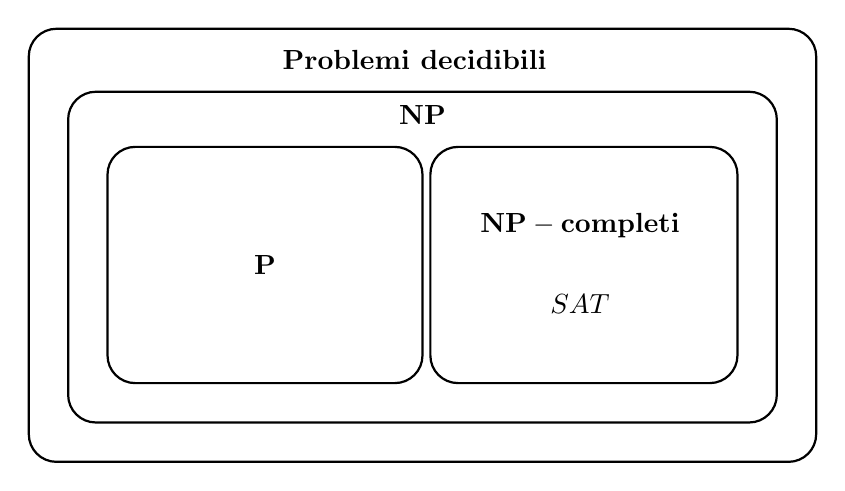
\begin{tikzpicture}[scale=1.0]
		\draw[black,rounded corners=10,thick]
		(0,0) rectangle (10,5.5);
		\draw[black,rounded corners=10,thick]
		(4.9,5.1) node {\bf Problemi decidibili};

		\draw[black,rounded corners=10,thick]
		(0.5, 0.5) rectangle (9.5,4.7);
		\draw[black,rounded corners=10,thick]
		(5,4.4) node {$\mathbf{\mathbf{NP}}$};

		\draw[black,rounded corners=10,thick]
		(1,1) rectangle (5,4);
		\draw[black,rounded corners=10,thick]
		(3,2.5) node {$\mathbf{\mathbf{P}}$};

		\draw[black,rounded corners=10,thick]
		(5.1,1) rectangle (9,4);
		\draw[black,rounded corners=10,thick]
		(7,3) node {\bf $\mathbf{NP-completi}$};
		\draw[black,rounded corners=10,thick]
		(7,2) node {$SAT$};

	\end{tikzpicture}
	\caption{Classi di complessità strutturale.}
	\label{fig:structcomplclass}
\end{figure}

\subsubsection{Riducibilità}
Il concetto di \textbf{riducibilità} (in tempo polinomiale) gioca una parte
fondamentale nella teoria della complessità strutturale: si dice che un problema $\Pi_1$
è polinomialmente riducibile ad un problema $\Pi_2$ se e solo se
$$
	\exists f: 2^* \rightarrow 2^*
$$
tale che:
\begin{itemize}
    \setlength\itemsep{0pt}
	\item $f$ è calcolabile polinomialmente
	\item $\forall x \in I_{\Pi_1}  ~~ f(x) \in I_{\Pi_2}$
	\item $\forall x ~~ Sol_{\Pi_2}(x) = 1 \iff Sol_{\Pi_1}(x) = 1$
\end{itemize}

Questa definizione ha come conseguenza il seguente lemma.
\begin{lemma}\label{lem:poli_red}
	Se $\Pi_2 \in \mathbf{P}$ e $ \Pi_1 \leq_{p} \Pi_2$,
	ossia $\Pi_1$ è riducibile polinomialmente a $\Pi_2$, allora $\Pi_1 \in \mathbf{P}$.
\end{lemma}
La classe dei problemi $\mathbf{NP-completi}$ è quindi definita come
$$
	\mathbf{NP-completi} = \{\Pi \in \mathbf{NP} | \forall \Pi'\in \mathbf{NP} ~~ \Pi' \leq_{p} \Pi\}
$$
\begin{theorem}[di Cook]
	$SAT \in \mathbf{NP-completi}$.
\end{theorem}
\chapter{Problemi di ottimizzazione}
\section {Introduzione}
Un problema di \textbf{ottimizzazione} è caratterizzato da: 
\begin{enumerate}
  \item  è l'insieme degli input $I_{\Pi}$;
  \item  è l'insieme degli output $O_{\Pi}$;
  \item  una funzione che ad ogni input associa una famiglia di output: $Amm_{\Pi} : I_{\Pi} \rightarrow \{2^{O_{\Pi}} \setminus \emptyset \}$;
  \item il tipo del problema $Tipo_{\Pi} \in \{Min, Max\}$; e
  \item una funzione da una coppia input-output ai naturali
    $$
	c_{\Pi}: I_{\Pi}\times O_{\Pi} \rightarrow \mathbb{N}
    $$
    che formalizza il concetto di \textbf{costo} di una soluzione - per un problema 
    di minizzazione, l'obiettivo sarà scegliere l'output con costo minore. 

\end{enumerate}
Le proprietà $3$, $4$ e $5$ formalizzano ulteriormente l'insieme $Sol_{\Pi}$ definito in precedenza. 
\subsection{Esempi}
\subsubsection{MaxSat}

\popt{MaxSAT}
{CNF ben formate}
{$\mathbb{N}$} 
{Qual è il numero massimo di clausole che si possono verificare?} 
{Assegnamenti di valori di verità coerenti} 
{$Max$}
{Numero di clausole rese vere}

\noindent
Le istanze di questo problema sone formule in forma normale congiunta ben formate
(ossia CNF); le soluzioni ammissibili sono assegnamenti di valori di verità; 
il costo (o \textit{funzione obiettivo}) è il numero di clausole rese vere. 
\textsc{MaxSat} ha chiaramente $Tipo_{\Pi} = Max$, in quanto 
l'obiettivo è massimizzare il numero di clausole verificate.

In alcuni frangenti potrebbe causarsi una certa ambiguità: 
l'algoritmo cerca \textit{il valore} della soluzione ottimale o \textit{la soluzione} ottimale stessa? 
Possiamo affermare che cerchiamo la soluzione stessa (in quanto il suo valore 
è calcolabile con la funzione di costo) e la indicheremo con la notazione $y^*(x)$; 
inoltre, indicheremo il costo della soluzione ottimale con $c^*(x)$.

\section{Rapporto di prestazioni}
Dato un input $x \in I_{\Pi}$ e $y \in Amm_{\Pi}$, possiamo sempre affermare che 
$$
\begin{cases}
  c_{\Pi}(x,y) \geq c_{\Pi}(x,y^*(x)) = c_{\Pi}^*(x) & \text{ per i problemi di minimo} \\
  c_{\Pi}(x,y) \leq c_{\Pi}(x,y^*(x)) = c_{\Pi}^*(x) & \text{ per i problemi di massimo}
\end{cases}
$$
\subsection{Rapporto di approssimazione}
Definiamo \textbf{rapporto di approssimazione} la quantità
$$
R_{\Pi}(x,y) = \max\{\frac{c_{\Pi}(x,y)}{c_{\Pi}(x, y^*(x))}, \frac{c_{\Pi}(x,y^*(x))}{c_{\Pi}(x, y)}\}
$$
questo valore ci permette di dimenticare se stiamo trattando un problema di 
minimizzazione o massimizzazione, in quanto sarà sempre $R_{\Pi} \geq 1$.

\subsubsection{$\alpha$-approssimazione}
Se, per esempio, $R_{\Pi} = 1$, la soluzione $y$ è in realtà $y = y^*(x)$; 
se $R_{\Pi} = 2$, per un problema di minimo significa che il costo di $y$ è 
il doppio del costo di $y^*(x)$, mentre per un problema di massimo significa che 
il costo di $y$ è la metà del costo di $y^*(x)$. 
In generale, dato un problema di approssimazione tenteremo di progettare
un algoritmo che preso un input $x \in I_{\Pi}$ produca un output $y(x) \in Amm_{\Pi}$. 
Se si riesce a dimostrare che l'algoritmo costruito trova una soluzione che, 
per ogni input $x$, è tale per cui $R(x,y(x)) \leq \alpha$ si definisce l'algoritmo 
$\alpha$-approssimato.

\section{Classi di complessità per l'ottimizzazione}
Considereremo sempre algoritmi che terminano in tempo polinomiale; ovviamente, 
vorremmo trovare un $\alpha$ il più piccolo possibile - l'obiettivo quindi non sarà
più migliorare il polinomio, bensì migliorare il grado di approssimazione $\alpha$
trovando il più piccolo possibile. 

La classe dei problemi approssimabili in modo esatto ($\alpha = 1$) 
in tempo polinomiale è chiamata $\mathbf{PO}$; si noti che non è una classe 
ristretta ai problemi di decisione - questa è infatti l'analogo della 
classe $\mathbf{P}$ rispetto ai problemi di ottimizzazione. 
Allo stesso modo possiamo definire una classe dei problemi 
di ottimizzazione risolvibili con approssimazione $1$ in tempo nondetermistico 
polinomiale: $\mathbf{NPO}$ è la classe definita dai 
problemi $\Pi = (I_{\Pi}, O_{\Pi}, Amm_{\Pi}, c_{\Pi})$ tali per cui
\begin{enumerate}
  \item esiste un polinomio $Q$ tale che $\forall x \in I_{\Pi} \forall y \in Amm_{\Pi}(x) ~~ |y| \leq Q(|x|)$,
  \item dato $x \in I_{\Pi}$ e $y \in 2^*$ con $|y| \leq Q(|x|)$ è decidibile in
    tempo polinomiale se $y \in Amm_{\Pi}$, e
  \item $c_{\Pi}$ è calcolabile in tempo polinomiale
\end{enumerate}
Nonostante questa classe non sia definita in termini di MdT con modulo nondetermistico (in quanto 
questo modello è ``démodée'': la teoria della complessità moderna utilizza al loro 
posto il concetto di \textit{testimoni}) la definizione è completamente analoga e
riconducibile alle definizioni che ne fanno uso.

\subsection{Classe di problemi $\mathbf{NPO-completi}$}
Tra la classe $\mathbf{PO}$ e $\mathbf{NPO}$ sussiste la stessa relazione 
che c'è tra $\mathbf{P}$ e $\mathbf{NP}$ - effettivamente, possiamo anche definire 
i problemi $\mathbf{NPO-completi}$. Per arrivare a questa definizione occorre 
definire la nozione di \textit{problema di decisione associato}: dato un problema 
di ottimizzazione $\Pi$, definiamo un problema di decisione $\hat{\Pi}$ associato 
a $\Pi$ definendo 
$$
I_{\hat{\Pi}} = I_{\Pi} \times \mathbb{N}
$$ 
che formalizza la \textit{richiesta} ``esiste una soluzione ammissibile 
per $x$ con costo minore o uguale a $k$?'' (o maggiore o uguale per i problemi 
di massimizzazione). 

\begin{theorem}
 $$
 \Pi \in \mathbf{PO} \implies \hat{\Pi} \in \mathbf{P}
 $$
 $$
 \Pi \in \mathbf{NPO} \implies \hat{\Pi} \in \mathbf{NP}
 $$
\end{theorem}

\noindent
Analogamente, la classe dei problemi $\mathbf{NPO-completi}$ è 
$$
\mathbf{NPO-completi} = \{\Pi \in \mathbf{NPO} | \hat{\Pi} \in \mathbf{NP-completi}\}
$$
Ed è corretto aspettarsi che il problema di inclusione di $\mathbf{NP}$ in $\mathbf{P}$ 
venga mantenuto anche per i problemi di ottimizzazione:
\begin{theorem}
  Se $\Pi \in \mathbf{NPO-completi}$, allora $\Pi \notin \mathbf{PO}$ a meno che
$\mathbf{P} = \mathbf{NP}$.
\end{theorem}

\begin{proof}
Assumiamo $Tipo_{\Pi} = Max$. Per assurdo, supponiamo $\Pi \in \mathbf{PO}$. 
dato un input $(x,k) \in I_{\Pi} \times \mathbb{N}$ calcoliamo la soluzione ottima 
$y^*(x)$ in tempo polinomiale usando il fatto che $\Pi \in \mathbf{PO}$. 
Se $k \leq c_{\Pi}(x, y^*(x))$ 
rispondiamo \textit{sì}, altrimenti rispondiamo \textit{no}. Questo algoritmo funziona in 
tempo polinomiale e decide il problema di decisione associato a $\Pi$; 
in quanto $\hat{\Pi} \in \mathbf{NP-completi}$, concludiamo $\mathbf{P} = \mathbf{NP}$.
\end{proof}

\subsection{Altre classi di complessità}
In base al rapporto di approssimazione e al comportamento 
dell'algoritmo dati gli input e il rapporto di approssimazione stesso è 
possibile definire ulteriori classi di complessità. Utilizziamo ora 
la notazione $A_{\Pi}$ per denotare un algoritmo che risolve il problema 
$\Pi$.

\subsubsection{La classe \textbf{APX}}
La classe dei problemi \textit{approssimabili} in tempo nondeterministico polinomiale:
$$
\mathbf{APX} = \{\Pi | \exists A_{\Pi}, \alpha: A_{\Pi} \text{ è } \alpha\text{-approssimante per } \Pi\}
$$
Abbiamo che $\mathbf{APX} \subsetneq \mathbf{NPO}$: vi sono infatti alcuni 
problemi che non sono approssimabili. 

\subsubsection{La classe {\bf PTAS}}
La seguente classe è parametrizzata dal valore del rapporto di approssimazione 
scelto:
$$
\mathbf{PTAS} = \{\Pi | \exists A_{\Pi},  (x, \rho) \in I_{\Pi} \times \mathbb{Q}^{\geq 1}:
A_{\Pi}(x) = y \in Amm_{\Pi}(x) \text{ in tempo } poly(x) \land R_{\Pi}(x,y) \geq \rho \} 
$$
Abbiamo che  $\mathbf{PTAS} \subsetneq \mathbf{APX}$, infatti vi sono problemi 
che non possono essere approssimati al più di un certo valore. Si noti che 
i problemi in $\mathbf{PTAS}$ sono risolti in tempo polinomiale \textit{nell'input} ma 
non nel valore di approssimazione stesso. 
\subsubsection{La classe {\bf FPTAS}}
Stringendo la restrizione di polinomialità anche sul rapporto di approssimazione 
otteniamo la seguente classe: 
$$
\mathbf{FPTAS} =  \{ \Pi | \Pi \in \mathbf{PTAS} \land A_{\Pi} \text{ termina in tempo } poly(x, \rho)\}
$$
Abbiamo che  $\mathbf{FPTAS} \subsetneq \mathbf{PTAS}$, infatti vi sono problemi 
che possono essere approssimati arbitrariamente solo utilizzando un tempo non 
polinomiale nel valore di approssimazione. 




\begin{figure}[h]
  \centering



\tikzset{every picture/.style={line width=0.75pt}} %set default line width to 0.75pt        

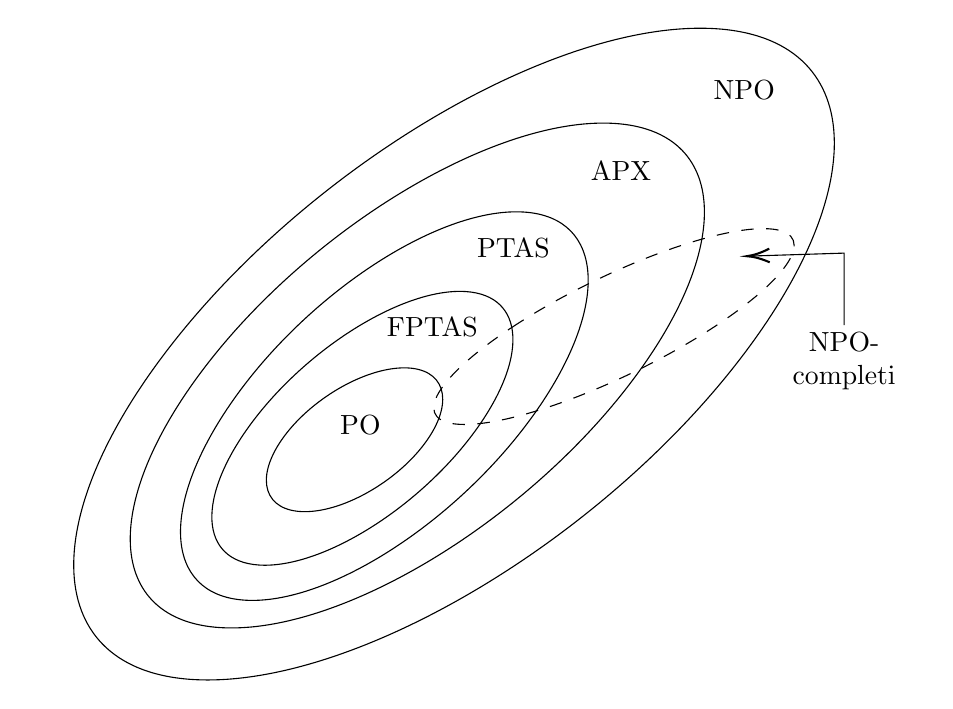
\begin{tikzpicture}[x=0.75pt,y=0.75pt,yscale=-1,xscale=1]
%uncomment if require: \path (0,477); %set diagram left start at 0, and has height of 477

%Shape: Ellipse [id:dp4588658322810296] 
\draw   (310.61,174.5) .. controls (376.13,87.79) and (491.77,17.5) .. (568.88,17.5) .. controls (645.98,17.5) and (655.37,87.79) .. (589.84,174.5) .. controls (524.31,261.21) and (408.68,331.5) .. (331.57,331.5) .. controls (254.46,331.5) and (245.08,261.21) .. (310.61,174.5) -- cycle ;
%Shape: Ellipse [id:dp4441062862246874] 
\draw   (327.15,184.82) .. controls (376.62,117.65) and (463.91,63.2) .. (522.11,63.2) .. controls (580.32,63.2) and (587.41,117.65) .. (537.94,184.82) .. controls (488.48,251.99) and (401.19,306.44) .. (342.98,306.44) .. controls (284.77,306.44) and (277.68,251.99) .. (327.15,184.82) -- cycle ;
%Shape: Ellipse [id:dp42532014972954124] 
\draw   (341.82,199.56) .. controls (376.94,147.86) and (438.92,105.95) .. (480.25,105.95) .. controls (521.58,105.95) and (526.61,147.86) .. (491.49,199.56) .. controls (456.37,251.26) and (394.39,293.17) .. (353.06,293.17) .. controls (311.73,293.17) and (306.7,251.26) .. (341.82,199.56) -- cycle ;
%Shape: Ellipse [id:dp9403889034822421] 
\draw   (350.81,210.25) .. controls (376.75,173.81) and (422.52,144.28) .. (453.04,144.28) .. controls (483.57,144.28) and (487.28,173.81) .. (461.34,210.25) .. controls (435.4,246.68) and (389.63,276.22) .. (359.11,276.22) .. controls (328.58,276.22) and (324.87,246.68) .. (350.81,210.25) -- cycle ;
%Shape: Ellipse [id:dp9056149450292196] 
\draw   (367.2,215.78) .. controls (380.43,196.64) and (406.86,181.13) .. (426.24,181.13) .. controls (445.62,181.13) and (450.6,196.64) .. (437.38,215.78) .. controls (424.15,234.91) and (397.71,250.42) .. (378.34,250.42) .. controls (358.96,250.42) and (353.97,234.91) .. (367.2,215.78) -- cycle ;
%Shape: Ellipse [id:dp18032210948172078] 
\draw  [dash pattern={on 4.5pt off 4.5pt}] (478.73,161.23) .. controls (518.48,135.18) and (572.44,114.06) .. (599.25,114.06) .. controls (626.06,114.06) and (615.57,135.18) .. (575.82,161.23) .. controls (536.07,187.29) and (482.11,208.41) .. (455.3,208.41) .. controls (428.48,208.41) and (438.98,187.29) .. (478.73,161.23) -- cycle ;
%Straight Lines [id:da10034962558485494] 
\draw    (638.18,160.5) -- (638.18,125.85) -- (593.29,127.26) ;
\draw [shift={(591.29,127.33)}, rotate = 358.2] [color={rgb, 255:red, 0; green, 0; blue, 0 }  ][line width=0.75]    (10.93,-3.29) .. controls (6.95,-1.4) and (3.31,-0.3) .. (0,0) .. controls (3.31,0.3) and (6.95,1.4) .. (10.93,3.29)   ;

% Text Node
\draw (574.07,41.64) node [anchor=north west][inner sep=0.75pt]   [align=left] {NPO};
% Text Node
\draw (514.9,80.38) node [anchor=north west][inner sep=0.75pt]   [align=left] {APX};
% Text Node
\draw (460.1,117.56) node [anchor=north west][inner sep=0.75pt]   [align=left] {PTAS};
% Text Node
\draw (416.67,155.6) node [anchor=north west][inner sep=0.75pt]   [align=left] {FPTAS};
% Text Node
\draw (394.14,202.63) node [anchor=north west][inner sep=0.75pt]   [align=left] {PO};
% Text Node
\draw (638.18,178) node   [align=left] {\begin{minipage}[lt]{51.43pt}\setlength\topsep{0pt}
\begin{center}
NPO-completi
\end{center}

\end{minipage}};


\end{tikzpicture}
\caption{Rappresentazione insiemistica delle classi di complessità.}
\label{fig:compsets}
\end{figure}



\section{Terminologia riguardante i problemi}
\subsection{Grafi}
I grafi non orientati sono $G=(V,E)$ (vertici e lati), dove 
$$
E \in {V\choose{2}}
$$
Il \textbf{grado} di un vertice $x$ $d(x)$ è il numero di lati incidenti su 
tale vertice. Il numero di vertici è $n = |V|$, mentre $m = |E|$. 
In un grafo non orientato un \textbf{cammino} di lunghezza $k$ 
$$
\pi = v_1, v_2, \cdots, v_k
$$
tale che $\forall v_{i} \in \pi :\exists \{v_i, v_{i+1}\} \in E$. 
Un cammino senza ripetizioni di vertici è chiamato \textit{semplice}, altrimenti
è definito \textit{non semplice}. Un \textbf{circuito} è un cammino semplice 
chiuso di lunghezza $\geq 3$. La \textbf{connessione} tra due vertici $x$ e $y$
è denotata $x \leadsto y$ e sussiste se esiste un cammino da $x$ a $y$ 
(e, di conseguenza, da $y$ a $x$); 
questa nozione è inoltre una relazione di equivalenza (totale), gode infatti 
di riflessività, transitività e simmetria. Gli insiemi di vertici mutuamente 
connessi formano le \textbf{componenti connesse} di un grafo.

\chapter{Algoritmi deterministici}



\section{\BiMaxMatching}\label{sec:BiMaxMatching}
Sia $G=(V,E)$ un grafo non orientato. Un \emph{matching} (matrimonio) in $G$ è una selezione $X$ di lati in $E$ tale che su nessun vertice in $V$ incide più di un lato di $X$.
\MaxMatching è il problema di trovare il matching di cardinalità massima in un dato grafo.

\BiMaxMatching è una versione di \MaxMatching su grafi bipartiti, cioè in cui i vertici sono divisi in due classi e ogni lato incide su un vertice per classe: $G=(V_1,V_2,E)$ dove $V_1\cap V_2=\emptyset$ e $E\subseteq V_1\times V_2$. $\BiMaxMatching\in\PO$.

\popt{\BiMaxMatching}
{Grafo bipartito $G=(V_1,V_2,E)$}
{$X\subseteq E$}
{Determinare il matching di cardinalità massima in $G$}
{$X\subseteq E:\forall e_1,e_2\in X,~ e_1\cap e_2\neq\emptyset\impl e_1=e_2$}
{$\MAX$}
{$\card X$}

\begin{figure}
	\centering
	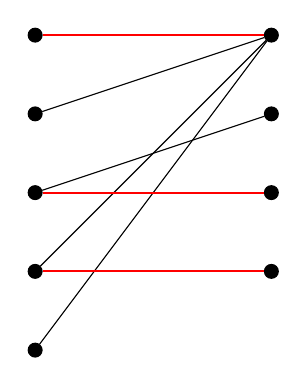
\begin{tikzpicture}[every node/.style={draw,inner sep=0pt,minimum size=5pt,fill,circle},matching/.style={red,thick}]
	\node at (0,1) (a) {};
	\node at (0,2) (b) {};
	\node at (0,3) (c) {};
	\node at (0,4) (d) {};
	\node at (0,5) (e) {};

	\node at (3,2) (f) {};
	\node at (3,3) (g) {};
	\node at (3,4) (h) {};
	\node at (3,5) (i) {};

	\draw		(a) -- (i);
	\draw		(b) -- (i);
	\draw		(d) -- (i);
	\draw[matching]	(e) -- (i);
	\draw[matching]	(b) -- (f);
	\draw[matching]	(c) -- (g);
	\draw		(c) -- (h);
\end{tikzpicture}

	\caption{Esempio di grafo bipartito. I lati colorati rappresentano un possibile matching.}
	\label{fig:graphmatching}
\end{figure}

Fissato un matching $M\subseteq E$, un lato $l\in E$ si dice \emph{occupato} se $l\in M$ e \emph{libero} se $l\notin M$.
Un vertice si dice \emph{esposto} se e solo se su di esso incidono solo lati liberi. Un cammino semplice si dice \emph{aumentante} rispetto a un matching se alterna lati liberi e occupati e inizia e termina su vertici esposti.
Quando un matching ha un cammino aumentante si può fare un \flang{flip}, cioè invertire l'appartenenza al matching dei lati del cammino aumentante.

\begin{figure}
	\centering
	\begin{subfigure}[b]{0.4\textwidth}
		\centering
		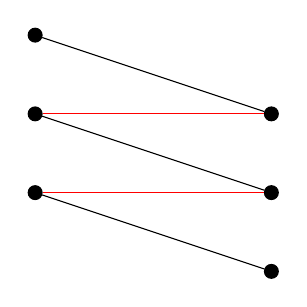
\begin{tikzpicture}
	\node[draw,inner sep=0pt,minimum size=5pt,fill, circle] at (3, 1)  (a) {};
	\node[draw,inner sep=0pt,minimum size=5pt,fill, circle] at (0, 2)  (b) {};
	\node[draw,inner sep=0pt,minimum size=5pt,fill, circle] at (0, 3)  (c) {};
	\node[draw,inner sep=0pt,minimum size=5pt,fill, circle] at (3, 2)  (f) {};
	\node[draw,inner sep=0pt,minimum size=5pt,fill, circle] at (3, 3)  (g) {};
	\node[draw,inner sep=0pt,minimum size=5pt,fill, circle] at (0, 4)  (h) {};

	\draw (a) -- (b);
	\draw[red] (b) -- (f);
	\draw (f) -- (c);
	\draw[red] (c) -- (g);
	\draw (g) -- (h);
\end{tikzpicture}

		\subcaption{Prima del flip.}
	\end{subfigure}
	\begin{subfigure}[b]{0.4\textwidth}
		\centering
		\input{img/matching_aumentante_post.tikz}
		\subcaption{Dopo il flip.}
	\end{subfigure}
	\caption{Esempio di cammino aumentante in un grafo bipartito.}
	\label{fig:augpaths}
\end{figure}

Vale il seguente teorema relativo ai cammini aumentanti per matching su grafi:
\begin{theorem}
	Sia $M$ un matching per un grafo $G$. Allora:
	\begin{equation*}
		\text{Esiste un cammino aumentante per $M$} \iff \text{$M$ non è massimo per $G$.}
	\end{equation*}
\end{theorem}
\begin{proof}~
	\begin{description}
		\item[$\Rightarrow$)] Applicando un flip al cammino aumentante si aumenta il matching di $1$.
		\item[$\Leftarrow$)] Se $M$ non è massimo, sia $M'$ un matching massimo per $G$ e sia $X:=(M\setminus M')\cup(M'\setminus M)$ (la differenza simmetrica di $M$ e $M'$).
			Su ogni vertice di $G$ possono incidere al più $2$ lati di $X$ (uno per ciascuno dei due matching).
			Nel grafo indotto da $X$, in ogni circuito l'appartenenza dei lati a $M$ e $M'$ è alternata e quindi il circuito è composto dallo stesso numero di lati di $M$ e di $M'$.
			Siccome però $M'$ ha più lati di $M$, esiste almeno un cammino semplice nel grafo indotto da $X$ che ha più lati in $M'$.
			Tale cammino alterna lati di $M$ e di $M'$ ed è aumentante rispetto a $M$ in $G$.
	\end{description}
\end{proof}

% TODO: è necessario discutere di come viene effettuata la visita per FindAugmenting e quale sia la sua complessità.
\SetKwFunction{FindAugmenting}{FindAugmenting}
\SetKwFunction{Flip}{Flip}
L'algoritmo \ref{alg:BiMaxMatching} risolve \BiMaxMatching trovando l'ottimo in tempo polinomiale.
La procedura \FindAugmenting tiene traccia dei vertici esposti e fa una visita in profondità del grafo a partire da uno di essi, alternando lati liberi e occupati, identificando un cammino aumentante.
La procedura \Flip esegue un flip del matching dato.

\begin{algorithm}
	$M \asn \emptyset$\;
\While{}{
	$\pi\asn\FindAugmenting{G,M}$\;
	\If{$\pi=\bot$}{
		\Return $M$\;
	}\Else{
		$M\asn\Flip(M,\pi)$\;
	}
}

	\caption{Risoluzione polinomiale di \BiMaxMatching}
	\label{alg:BiMaxMatching}
\end{algorithm}

\begin{corollario}
	$\BiMaxMatching\in\PO$.
\end{corollario}

\PerfectMatching è il problema di decisione che si chiede se in un grafo bipartito esista un matching che coinvolge tutti i vertici.

\begin{corollario}
	$\PerfectMatching\in\P$.
\end{corollario}

% TODO: in relazione al todo precedente, spiegare perché l'algoritmo precedente non sia polinomiale su grafi generici e dire che in quel caso servono tecniche più avanzate per trovare cammini aumentanti.
Vale inoltre il seguente risultato, che non dimostriamo:
\begin{theorem}
	$\MaxMatching\in\PO$.
\end{theorem}



\section{\LoadBalancing}
Il problema \LoadBalancing (bilanciamento del carico) consiste nel dividere un insieme di task, ciascuno con la sua durata, tra le macchine di un insieme, in modo da minimizzare la durata complessiva (carico) impiegata dalla macchina più carica. Questo problema è \NPO-completo.

\popt
{\LoadBalancing}
{Durate $t_0,\dots,t_{n-1}\in\N^+$ per $n$ task, numero $m$ di macchine}
{Assegnamento di ciascun task a una macchina}
{Determinare l'assegnamento che minimizza la durata massima}
{Assegnamenti $x:n\to m$}
{$\MIN$}
{$L=\max_j L_j$, dove $L_j:=\sum_{i\in x^{-1}(j)} t_i$}


\subsection{\GreedyLoadBalancing}
Un algoritmo greedy può trovare una soluzione ammissibile per \LoadBalancing.
L'algoritmo esamina i task $t_0,t_1,\dots,t_{n-1}$ nell'ordine, assegnando ogni task alla macchina più scarica.
\GreedyLoadBalancing, se implementato con una coda con priorità che tenga conto della macchina dal carico minimo (effettuando $n$ operazioni di insert/update per i carichi di $m$ macchine), opera in tempo $O(n\log m)$.
L'algoritmo non ottiene, in generale, la soluzione ottima, ma ha la garanzia di non produrre più del doppio dell'ottimo, come dimostrato dal seguente teorema:

\begin{theorem}\label{thm:greedyloadbalancing}
	\GreedyLoadBalancing è un algoritmo 2-approssimante per \LoadBalancing.
\end{theorem}
Prima di dimostrare il teorema si consideri il seguente lemma:
\begin{lemma}\label{lem:load:ultimopasso}
	Sia $L\star$ il costo della soluzione ottima. Sia $\bar j$ tale che $L_{\bar j}=L\star$ e sia $\bar i$ l'ultimo task assegnato a $\bar j$. Allora:
	\begin{equation*}
		L_{\bar j}-t_{\bar i} \leq L\star
	\end{equation*}
\end{lemma}
\begin{proof}
	Il carico della macchina $\bar j$ prima dell'assegnamento $\bar i$ era $L_{\bar j}-t_{\bar i}$, il cui era minore di ogni altro carico per via di come l'algoritmo sceglie a chi assegnare.
	Indicato con $L\star_j$ il carico della macchina $j$ nella soluzione ottima, vale $L\star\geq\frac1m\sum_it_i$, essendo $mL\star\geq\sum_jL\star_j=\sum_it_i$.
	\begin{gather*}
		L_{\bar j}-t_{\bar i}\leq L_j \qquad\forall j \\
		\sum_j (L_{\bar j}-t_{\bar i})\leq\sum_j L_j=\sum_i t_i\\
		m(L_{\bar j}-t_{\bar i})\leq \sum_i t_i \\
		L_{\bar j}-t_{\bar i}\leq\frac1m\sum_j t_j\leq L\star
	\end{gather*}
\end{proof}
Si può ora procedere con la dimostrazione del teorema \ref{thm:greedyloadbalancing}:
\begin{proof}
	Si osservi che $L\star\geq\max_it_i$. Applicando il lemma \ref{lem:load:ultimopasso}:
	\begin{gather*}
		L=L_{\bar j}=\underbrace{L_{\bar j}-t_{\bar i}}_{\leq L\star}+\underbrace{t_{\bar i}}_{\leq L\star}\leq 2L\star \\[1ex]
		\frac L{L\star}\leq 2
	\end{gather*}
\end{proof}

\begin{corollario}
	$\LoadBalancing\in\gAPX2$.
\end{corollario}

Si dimostra che questo risultato sull'analisi di \GreedyLoadBalancing è tight:
\begin{theorem}
	Per ogni $\varepsilon>0$ esiste un input di \LoadBalancing su cui \GreedyLoadBalancing produce una soluzione $L$ tale che
	\begin{equation*}
		2-\varepsilon\leq\frac L{L\star}
	\end{equation*}
\end{theorem}
\begin{proof}
	Scegliamo un numero di macchine $m\geq\frac1\varepsilon$ e un numero di task $n=m(m-1)+1$. Questi task consistono, nell'ordine, in $n-1$ task di durata $1$ e un task da $m$. Naturalmente la soluzione ottima assegna unicamente il task da $m$ a una macchina, che risulta la più carica, quindi $L\star=m$.

	Per assegnare i task, l'algoritmo assegna un task da $1$ per ogni macchina ciclicamente finché arriva il task da $m$, che viene assegnato a una macchina di carico $m-1$ producendo un costo finale di $2m-1$. In questo caso si ha
	\begin{equation*}
		\frac L{L\star}=\frac{2m-1}{m}=2-\frac1m\geq2-\varepsilon
	\end{equation*}
\end{proof}


\subsection{\SortedGreedyBalance}
Un algoritmo \SortedGreedyBalance può ordinare i task in ordine decrescente prima di assegnarli come \GreedyLoadBalancing. Questo algoritmo ha costo in tempo di $O(n\log n+n\log m)$.

\begin{theorem}
	\SortedGreedyBalance è un algoritmo $\frac32$-approssimante per \LoadBalancing.
\end{theorem}
\begin{proof}
	Se $n\leq m$, a ciascuna macchina viene assegnato un solo task, quindi $L=L\star=\max_i t_i$. La tesi, pertanto, è ovvia.

	Se $n>m$, esiste una macchina che riceve due task.
	Il primo task assegnato a una macchina già carica è $m$.
	Poiché esistono $m$ task di durata superiore a $t_m$, anche nella soluzione ottima due di essi devono essere assegnati alla stessa macchina (principio della piccionaia), quindi vale:
	\begin{equation*}
		L\star\geq 2t_m \text.
	\end{equation*}

	Sia $\bar j$ una macchina con carico massimo al termine dell'esecuzione e $\bar i$ l'ultimo task assegnatovi.
	Se $\bar i$ è l'unico task di $\bar j$, allora la soluzione è ottima e la tesi è ovvia.
	In ogni altro caso si ha $\bar i \geq m$, da cui $t_{\bar i}\leq t_m$ e quindi $t_{\bar i}\leq t_m\leq \frac12 L\star$.
	\begin{gather*}
		L=\underbrace{L_{\bar j}-t_{\bar i}}_{\leq L\star}+\underbrace{t_{\bar i}}_{\leq \frac12 L\star}\leq L\star+\frac12 L\star=\frac32L\star
	\end{gather*}
\end{proof}

Valgono inoltre i seguenti teoremi riguardanti \LoadBalancing, che non dimostriamo.
\begin{theorem}~
	\begin{itemize}
		\item \SortedGreedyBalance è un algoritmo $\frac43$-approssimante per \LoadBalancing \cite{Graham:69:sortedgreedybalance};
		\item $\LoadBalancing\in\PTAS$;
		\item $\P\neq\NP\impl\LoadBalancing\notin\FPTAS$.
	\end{itemize}
\end{theorem}



\section{\CenterSelection}
Nel problema \CenterSelection è dato uno spazio metrico $\tuple{S,d}$.
Tra i punti si $S$ si selezionano centri $C\subseteq S$: ogni punto ha un centro di riferimento che consiste nel più vicino.
La massima distanza tra un punto di $S$ e il suo centro di riferimento è detta raggio di copertura ed è il valore che si vuole minimizzare.
\CenterSelection è un problema \NPO-completo.

\popt{\CenterSelection}
{Spazio metrico $S$ con distanza $d$, numero massimo di centri $k\in\N^+$}
{$C\subseteq S$}
{Selezionare al più $k$ centri che minimizzino il raggio di copertura}
{$C\subseteq S\mid \card C\leq k$}
{$\MIN$}
{$\rho(C) = \max_{x \in S} d(x, C)$}

Uno spazio metrico è un insieme $\Omega$ di punti su cui vale una funzione distanza $d:\Omega\times\Omega\to\R^{\geq0}$ tale che:
\begin{itemize}
	\item $\forall x\in S\quad d(x,x)=0$
	\item $\forall x,y\in S\quad d(x,y)=d(y,x)$
	\item $\forall x,y,z\in S\quad d(x,y)\leq d(x,z)+d(z,y)$ (disuguaglianza triangolare)
\end{itemize}
Sia $C\subseteq\Omega$ e $s\in\Omega$. Con abuso di notazione si indica con $d(s,C)$ la distanza minima tra il punto $s$ e i punti appartenenti a $C$, ossia $d(s,C):=\min_{c\in C} d(s,c)$.

\begin{defin}[tassellatura di Voronoi]
	Dato uno spazio metrico $\tuple{\Omega,d}$, sia $S\subseteq\Omega$ finito e $C\subseteq S$ un insieme di centri.
	Dato un punto $s\in S$ il centro di riferimento di $s$ è $\text{VC}_C(s):=\arg\min_{c\in C} d(s,c)$.
	Per ogni $c\in C$, la cella di Voronoi di centro $c$ è l'insieme $\text{VC}_C^{-1}(c)$ degli elementi di $S$ mappati in $c$ tramite $\text{VC}_C$.
\end{defin}

\begin{equation*}
	\text{VC}_C(s)=\arg\min_{c\in C} d(s,c)
\end{equation*}

\CenterSelection è il problema che riceve in input $S\subseteq_\text{fin}\Omega$ e $k\in\N^+$, ha come soluzioni ammissibili le selezioni di centri $C\subseteq S$ con $\card C\leq k$ e come obiettivo da minimizzare:
\begin{equation*}
	\rho(C)=\max_{s\in S} d(s,\text{VC}_C(s))
\end{equation*}

\subsection{\CenterSelectionPlus}
L'algoritmo \ref{alg:CenterSelectionPlus} non risolve \CenterSelection in quanto richiede un input $r$ aggiuntivo rispetto a quelli previsti dal problema, che consiste in una stima del raggio di copertura ottimo $\rho\star$.

\begin{algorithm}[ht]
	\caption{\CenterSelectionPlus}
	\label{alg:CenterSelectionPlus}
	\SetKwFunction{ExtractRandomPoint}{ExtractRandomPoint}

\KwInput{$S$, $k$, $d$, $r$}

$C\asn\emptyset$\;
\While{$S \neq \emptyset$}{
	$\bar s\asn\ExtractRandomPoint(S)$\;
	$C\asn C\cup \set{\bar s}$\;
	$S\asn S\setminus\set{x\mid d(x,\bar s)\leq 2r}$\;
}
\If{$\card C\leq k$}{
	\Return $C$\;
}\Else{
	Impossibile\;
}

\end{algorithm}

\begin{theorem}
	Valgono le seguenti proprietà per \CenterSelectionPlus:
	\begin{enumerate}[(a)]
		\item \label{itm:centerselection:plus1} se l'algoritmo emette un output $C$, allora $C$ è una soluzione ammissibile con $\rho(C)\leq 2r$;
		\item \label{itm:centerselection:plus2} se $r\geq\rho\star$ allora l'algoritmo emette un output.
		\item \label{itm:centerselection:plus3} se $r<\frac{\rho\star}{2}$ allora l'algoritmo non produce un output.
	\end{enumerate}
\end{theorem}
\begin{proof}
	\ref{itm:centerselection:plus1} L'output $C$ è ammissibile in quanto composto da elementi di $S$ e $\card C\leq k$.
	Poiché l'algoritmo termina quando sono stati eliminati tutti i punti di $S$, e ogni punto $s\in S$ viene eliminato quando per un centro $\bar s$ selezionato vale $d(s,\bar s)\leq 2r$, il raggio massimo da un punto al centro più vicino è minore o uguale a $2r$;

	\ref{itm:centerselection:plus2} Sia $C\star$ una soluzione ottima. Si consideri $\bar s\in S$ e sia $\bar c:=\text{VC}_{C\star}(\bar s)$ e $X_{\bar c}:=\text{VC}_{C\star}^{-1}(\bar c)$.
	Per qualunque punto $s\in X_{\bar c}$ vale, per disuguaglianza triangolare:
	\begin{equation*}
		d(s,\bar s) \leq d(s,\bar c)+d(\bar c,\bar s) \leq \rho\star + \rho\star = 2\rho\star \leq 2r \text.
	\end{equation*}
	Quindi dopo l'inserimento di $\bar s$ non rimane in $S$ alcun elemento di $X_{\bar c}$.
	Poiché la soluzione ottima contiene al più $k$ centri, dopo al più $k$ iterazioni tutti i punti di $S$ sono stati rimossi, e $\card C\leq k$.

	\ref{itm:centerselection:plus3} Se l'algoritmo emettesse un output $C$ per $r<\frac{\rho\star}{2}$, allora per il punto \ref{itm:centerselection:plus1} si avrebbe $\rho(C)\leq 2r<\rho\star$, il che è assurdo se $\rho\star$ è l'ottimo.
\end{proof}


Come rappresentato in figura \ref{fig:csplus_r_beh}, l'algoritmo ricevendo $r\geq\rho\star$ produce una soluzione ammissibile con approssimazione $\frac{2r}{\rho\star}$; se $r<\frac{\rho\star}{2}$ l'algoritmo non produce output; nei casi rimanenti il comportamento dell'algoritmo non è consistente.
Un algoritmo del genere può essere utilizzato sfruttando un'opportuna applicazione della ricerca dicotomica per la determinazione del valore ottimo di $r$.

\begin{figure}[ht]
	\centering
	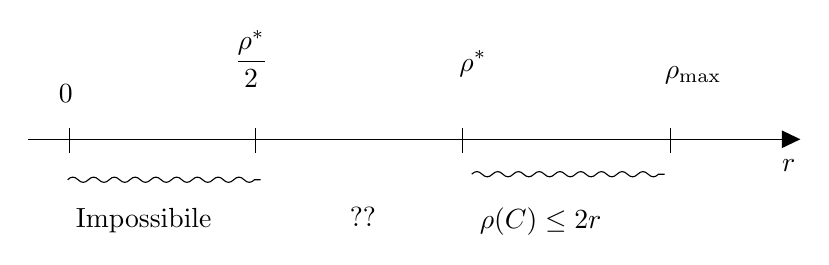
\begin{tikzpicture}[x=0.75pt,y=0.75pt,yscale=-1,xscale=1]
	\draw    (121,120.5) -- (490,120.5) ;
	\draw [shift={(493,120.5)}, rotate = 180] [fill={rgb, 255:red, 0; green, 0; blue, 0 }  ][line width=0.08]  [draw opacity=0] (8.93,-4.29) -- (0,0) -- (8.93,4.29) -- cycle    ;
	\draw    (230.33,115) -- (230.33,127) ;
	\draw    (330.33,115) -- (330.33,127) ;
	\draw    (430.33,115) -- (430.33,127) ;
	\draw    (140.75,115) -- (140.75,127) ;
	\draw    (140,140) .. controls (141.67,138.33) and (143.33,138.33) .. (145,140) .. controls (146.67,141.67) and (148.33,141.67) .. (150,140) .. controls (151.67,138.33) and (153.33,138.33) .. (155,140) .. controls (156.67,141.67) and (158.33,141.67) .. (160,140) .. controls (161.67,138.33) and (163.33,138.33) .. (165,140) .. controls (166.67,141.67) and (168.33,141.67) .. (170,140) .. controls (171.67,138.33) and (173.33,138.33) .. (175,140) .. controls (176.67,141.67) and (178.33,141.67) .. (180,140) .. controls (181.67,138.33) and (183.33,138.33) .. (185,140) .. controls (186.67,141.67) and (188.33,141.67) .. (190,140) .. controls (191.67,138.33) and (193.33,138.33) .. (195,140) .. controls (196.67,141.67) and (198.33,141.67) .. (200,140) .. controls (201.67,138.33) and (203.33,138.33) .. (205,140) .. controls (206.67,141.67) and (208.33,141.67) .. (210,140) .. controls (211.67,138.33) and (213.33,138.33) .. (215,140) .. controls (216.67,141.67) and (218.33,141.67) .. (220,140) .. controls (221.67,138.33) and (223.33,138.33) .. (225,140) .. controls (226.67,141.67) and (228.33,141.67) .. (230,140) -- (233,140) -- (233,140) ;
	\draw    (334.67,137.33) .. controls (336.34,135.66) and (338,135.66) .. (339.67,137.33) .. controls (341.34,139) and (343,139) .. (344.67,137.33) .. controls (346.34,135.66) and (348,135.66) .. (349.67,137.33) .. controls (351.34,139) and (353,139) .. (354.67,137.33) .. controls (356.34,135.66) and (358,135.66) .. (359.67,137.33) .. controls (361.34,139) and (363,139) .. (364.67,137.33) .. controls (366.34,135.66) and (368,135.66) .. (369.67,137.33) .. controls (371.34,139) and (373,139) .. (374.67,137.33) .. controls (376.34,135.66) and (378,135.66) .. (379.67,137.33) .. controls (381.34,139) and (383,139) .. (384.67,137.33) .. controls (386.34,135.66) and (388,135.66) .. (389.67,137.33) .. controls (391.34,139) and (393,139) .. (394.67,137.33) .. controls (396.34,135.66) and (398,135.66) .. (399.67,137.33) .. controls (401.34,139) and (403,139) .. (404.67,137.33) .. controls (406.34,135.66) and (408,135.66) .. (409.67,137.33) .. controls (411.34,139) and (413,139) .. (414.67,137.33) .. controls (416.34,135.66) and (418,135.66) .. (419.67,137.33) .. controls (421.34,139) and (423,139) .. (424.67,137.33) -- (427.67,137.33) -- (427.67,137.33) ;

	\draw (483,129) node [anchor=north west][inner sep=0.75pt]   [align=left] {$\displaystyle r$};
	\draw (134.5,93) node [anchor=north west][inner sep=0.75pt]   [align=left] {$\displaystyle 0$};
	\draw (219,67) node [anchor=north west][inner sep=0.75pt]   [align=left] {$\displaystyle \frac{\rho ^{*}}{2}$};
	\draw (327.5,76.5) node [anchor=north west][inner sep=0.75pt]   [align=left] {$\displaystyle \rho ^{*}$};
	\draw (426.5,84) node [anchor=north west][inner sep=0.75pt]   [align=left] {$\displaystyle \rho_{\max}$};
	\draw (142.67,152.67) node [anchor=north west][inner sep=0.75pt]   [align=left] {Impossibile};
	\draw (337.33,152) node [anchor=north west][inner sep=0.75pt]   [align=left] {$\rho(C)\leq 2r$};
	\draw (274.67,152) node [anchor=north west][inner sep=0.75pt]   [align=left] {??};
\end{tikzpicture}

	\caption{Comportamento di \CenterSelectionPlus.}
	\label{fig:csplus_r_beh}
\end{figure}


\subsection{\GreedyCenterSelection}
L'algoritmo \ref{algo:GreedyCenterSelection} è un algoritmo greedy per \CenterSelection.

\begin{algorithm}
	\caption{\GreedyCenterSelection}
	\SetKwFunction{ExtractRandomPoint}{ExtractRandomPoint}

\KwInput{$S$, $k$, $d$}

\If{$\card S\leq k$}{
	\Return $S$\;
}
$s\asn\ExtractRandomPoint(S)$\;
$C\asn C\cup \set{s}$\;
\While{$\card C\leq k$}{
	$\bar s\asn\arg\max_{s\in S} d(s,C)$\;
	$C\asn C\cup\set{\bar s}$\;
}
\Return $C$\;

	\label{algo:GreedyCenterSelection}
\end{algorithm}

\begin{theorem}
	\GreedyCenterSelection è un algoritmo $2$-approssimante per \CenterSelection.
\end{theorem}
\begin{proof}
	Si consideri una variante di \CenterSelectionPlus che, invece di eliminare punti di $S$, prenda in considerazione nella selezione di nuovi centri solo punti $s$ tali che $d(s,C)>2r$.
	Questo algoritmo \CenterSelectionPlus' è del tutto equivalente a \CenterSelectionPlus in quanto, selezionato un centro, i punti entro una distanza $2r$ da esso vengono ignorati per il resto della computazione.

	Per assurdo, supponiamo che l'output $C$ sia tale che $\rho(C)>2\rho\star$, ossia esiste $\hat s\in S$ tale che $d(\hat s,C)> 2\rho\star$.
	Consideriamo l'$i$-esima iterazione dell'algoritmo: sia $C_i$ l'insieme dei centri all'inizio dell'$i$-esima iterazione e $\bar s_i$ il centro da inserire.
	Per il funzionamento dell'algoritmo e poiché $C_i\subseteq C$, vale:
	\begin{equation*}
		d(\bar s_i,C_i)\geq d(\hat s,C_i)\geq d(\hat s, C)>2\rho\star
	\end{equation*}
	Quindi, il centro viene scelto tra quelli distanti almeno $2\rho\star$ dai centri attuali.
	L'algoritmo equivale quindi a un'esecuzione di \CenterSelectionPlus' con $r=\rho\star$.
	Ma per $r=\rho\star$ \CenterSelectionPlus' emette una $\frac{2\rho\star}{\rho\star}=2$-approssimazione, il che contraddice l'ipotesi di assurdo.
\end{proof}


\subsection{Inapprossimabilità di \CenterSelection}
\begin{theorem}
	Se $\P\neq\NP$, non esiste $\alpha<2$ tale che $\CenterSelection\in\gAPX\alpha$.
\end{theorem}
\begin{proof}
	Si consideri il problema di decisione \NP-completo \DominatingSet. Dato un grafo non orientato $G=(V,E)$, un dominating set per $G$ è un insieme di vertici $D\subseteq V$ se e solo se ogni vertice non appartenente a $D$ ha un adiacente in $D$: $\forall x\in(V\setminus D),\exists y\in D\mid \set{x,y}\in E$.

	\pdec{\DominatingSet}
	{Grafo non orientato $G=(V,E)$, $k\in\N^+$}
	{Determinare se esiste un dominating set per $G$ di cardinalità minore o uguale a $k$}

	Data un'istanza $((V,E),k)$ di \DominatingSet, costruiamo una istanza di \CenterSelection che ha per spazio l'insieme dei vertici, per numero massimo di centri il limite di cardinalità $k$ per il dominating set e per metrica la funzione
	\begin{equation*}
		d(x,y) =
		\begin{cases}
			0 \quad & \text{se } x = y                      \\
			1 \quad & \text{se } x\neq y\land\set{x,y}\in E \\
			2 \quad & \text{altrimenti}
		\end{cases}
	\end{equation*}
	Si noti che $d$ soddisfa la definizione di metrica.

	In una istanza di \CenterSelection derivata in questo modo, $\rho\star=2$ oppure $\rho\star=1$.
	Nel secondo caso l'insieme di centri scelti è un dominating set nell'istanza originale del problema.
	Infatti, sia $D\subseteq S$ la soluzione ottima per tale istanza. Vale:
	\begin{align*}
		\rho\star=1 & \coimpl\forall x\in(V\setminus D)\quad d(x,D)=1                             \\
		            & \coimpl\forall x \in (V \setminus D)\quad \exists y\in D\mid d(x,y)=1       \\
		            & \coimpl\forall x \in (V \setminus D)\quad \exists y\in D\mid \set{x,y}\in E \\
		            & \coimpl D\text{ è un dominating set}
	\end{align*}

	Per assurdo, supponiamo che esista un algoritmo polinomiale $\alpha$-approssimante per \CenterSelection, con $\alpha < 2$.
	Eseguendo tale algoritmo su un'istanza così costruita si ottiene un output $D$ tale che:
	\begin{gather*}
		1\leq\frac{\rho(D)}{\rho\star}\leq\alpha<2 \\
		\rho\star\leq\rho(D)\leq\alpha\cdot\rho\star<2\rho\star
	\end{gather*}

	Dato che $\rho\star=1\lor\rho\star=2$, allora vale esattamente una delle seguenti proposizioni:
	\begin{equation*}
		\begin{cases}
			1\leq\rho(D)<2\quad & \text{se } \rho\star=1 \\
			2\leq\rho(D)<4\quad & \text{se } \rho\star=2
		\end{cases}
	\end{equation*}
	Quindi, eseguito l'algoritmo, se $\rho(D)<2$ allora $\rho\star=1$ e la decisione per l'istanza originale di \DominatingSet è positiva; se $\rho(D)\geq2$ allora $\rho\star=2$ e la decisione è negativa.

	Poiché l'algoritmo agisce in tempo polinomiale, allora $\DominatingSet\in\P$, il che è assurdo se $\P\neq\NP$.
\end{proof}
Questa tecnica dimostrativa, consistente nel ridurre un problema \NP-completo e poterlo decidere in tempo polinomiale in ipotesi di assurdo discriminando di che intervallo fa parte la soluzione, è detta tecnica di riduzione con produzione di gap (\flang{gap-producing reduction}).



\section{\MinSetCover}\label{sec:SetCover}
Si definisce funzione armonica la funzione $H:\N^+\to\R$ tale che
\begin{equation*}
	H(n)=\sum_{k=1}^n \frac 1k
\end{equation*}

% TODO: dimostrare in un'appendice (vedi vecchi appunti)
Vale la seguente proprietà per la funzione armonica:
\begin{theorem}
	$\ln(n+1)\leq H(n)\leq 1+\ln n$.
\end{theorem}

Nel problema \MinSetCover sono dati insiemi, ciascuno con il suo peso, la cui unione è un insieme universo.
Il problema consiste nel trovare una selezione degli insiemi la cui unione copra l'intero insieme universo e il cui costo complessivo sia minimo.
\MinSetCover è un problema \NPO-completo.

\popt{\MinSetCover}
{$S_1,S_2,\dots,S_m\subseteq U$ tali che $\cup_{i=1}^m S_i=U$ e pesi $w_1,\dots,w_m$ con $w_i \in\Q^+~\forall i$}
{$C\subseteq\set{S_1,\dots,S_n}$}
{Determinare una selezione di insiemi che minimizzi il costo complessivo}
{$C$ tale che $\cup_{i\in C}S_i=U$}
{$\MIN$}
{$w:=\sum_{i:S_i\in C} w_i$}


\subsection{\GreedySetCover}
\begin{algorithm}[ht]
	\caption{\GreedySetCover}
	\label{algo:greedysetcover}
	\KwInput{$S_i, U$}

$R\asn U$\;
$C\asn\emptyset$\;
\While{$R\neq\emptyset$} {
	$i=\arg\min_i \set{\frac{w_i}{\card{S_i \cap R}}}$\;
	$C\asn C\cup\set{S_i}$\;
	$R\asn R\setminus S_i$\;
}
\Return{$C$}\;

\end{algorithm}
L'algoritmo \ref{algo:greedysetcover} costruisce polinomialmente una soluzione per \MinSetCover, scegliendo a ogni iterazione il sottoinsieme di input che minimizza il rapporto tra il suo peso e il numero di elementi che esso aggiunge all'output parziale.

Ogni elemento $s\in U$ viene inserito nell'output parziale in qualche iterazione $j$ con l'aggiunta di un sottoinsieme $S_j$. Definiamo quindi
\begin{equation*}
	c_u = \frac{w_j}{\card{S_j\cap R_j}}
\end{equation*}
il costo della copertura del singolo elemento di $U$, avvenuta tramite l'aggiunta di $S_j$ durante la $j$-esima iterazione.

\begin{lemma}\label{lem:gsetcov_w_sum_c_u}
	\begin{equation*}
		w=\sum_{u\in U} c_u
	\end{equation*}
\end{lemma}
\begin{proof}
	Si noti che gli insiemi $S_j\cap R_j$, dove $S_j$ è l'insieme di input scelto al passo $j$ e $R_j$ è l'insieme degli elementi dell'universo rimasti da selezionare al passo $j$, costituiscono una partizione di $U$. Infatti, l'algoritmo termina solo dopo aver esaurito gli elementi di $U$, e ogni insieme $S_j\cap R_j$ aggiunge unicamente nuovi elementi.

	Sia $w_j$ il costo dell'insieme $S_j$ aggiunto al passo $j$. Allora
	\begin{equation*}
		w = \sum_j w_j=\sum_j\sum_{s\in S_j\cap R_j} c_s=\sum_{u\in U} c_u
	\end{equation*}
\end{proof}
\begin{lemma}\label{lem:gsetcov_cu_leq_harmoskwk}
	\begin{equation*}
		\forall k\in\set{1,\dots,m} \quad\sum_{s\in S_k} c_s\leq H(\card{S_k}) \cdot w_k
	\end{equation*}
\end{lemma}
\begin{proof}
	Sia $S_k=\set{s_1,s_2,\dots,s_d}$, dove gli elementi sono elencati in ordine di copertura.

	Prima che un elemento $s_i$ venga coperto dall'inserimento di un insieme $S_{k'}$, gli elementi di $S_k$ ancora da inserire spaziano almeno da $s_i$ a $s_d$, quindi:
	\begin{equation*}
		\card{S_k\cap R_j}\geq d-i+1 \text.
	\end{equation*}
	Quindi
	\begin{equation*}
		c_{s_i}=\frac{w_{k'}}{\card{S_{k'}\cap R_j}}
		\leq\frac{w_k}{\card{S_k\cap R_j}}
		\leq\frac{w_k}{d-i+1} \text.
	\end{equation*}
	E, di conseguenza
	\begin{align*}
		\sum_{s\in S_k} c_s & =c_{s_1}+c_{s_2}+c_{s_3}\dots+c_{s_d}                            \\
		                    & \leq \frac{w_k}{d-1+1}+\frac{w_k}{d-2+1}+\dots+\frac{w_k}{d-d+1} \\
		                    & \leq \frac{w_k}{d}+\frac{w_k}{d-1}+\dots+\frac{w_k}{1}           \\
		                    & = w_k\left(1 + \frac{1}{2} + \dots + \frac{1}{d}\right)          \\
		                    & = w_k\cdot H(\card{S_k})
	\end{align*}
\end{proof}

\begin{theorem}
	Sia $M=\max_i\card{S_i}$. \GreedySetCover è $H(M)$-approssimante per \MinSetCover.
\end{theorem}
\begin{proof}
	Sia $w\star:=\sum_{i:S_i\in C\star} w_i$.
	Eseguito l'algoritmo, in virtù del lemma \ref{lem:gsetcov_cu_leq_harmoskwk} vale, per qualunque $i$:
	\begin{equation*}
		w_i\geq\frac{\sum_{s\in S_i} c_s}{H(\card{S_i})}\geq\frac{\sum_{s\in S_i} c_s}{H(M)}
	\end{equation*}
	Essendo $C\star$ una copertura e applicando il lemma \ref{lem:gsetcov_w_sum_c_u}:
	\begin{equation*}
		\sum_{S_i\in C\star}\sum_{s\in S_i} c_s \geq \sum_{s\in U} c_s = w
	\end{equation*}
	Applicando queste due osservazioni:
	\begin{gather*}
		w\star = \sum_{i:S_i\in C\star} w_i \geq \sum_{i:S_i\in C\star} \frac{\sum_{s\in S_i} c_s}{H(M)} \geq \frac{w}{H(M)} \\
		\frac{w}{w\star} \leq H(M)
	\end{gather*}
\end{proof}

Inoltre vale:
\begin{equation*}
	H(M)\leq H(\card U) = O(\log \card U)
\end{equation*}
Ergo:
\begin{corollario}
	\GreedySetCover è un algoritmo $O(\log n)$-approssimante per \MinSetCover, dove $n$ è la cardinalità dell'insieme universo.
\end{corollario}

Per quanto riguarda l'ottimalità di questo bound:
\begin{theorem}
	Per ogni $\varepsilon>0$, \GreedySetCover non è $(O(\log n)-\varepsilon)$-approssimante per \MinSetCover.
\end{theorem}
\begin{proof}
	% TODO: è necessario essere più precisi in questa costruzione: si può fare con qualunque n? È necessaria una potenza di 2? Gli insiemi S finali possono contenere un solo elemento o sempre almeno 2? Etc.
	Fissati $\varepsilon$ e $n$ (sia per semplicità $n=2^k$ per qualche $k\in\N^+,k>2$), si consideri l'input per \MinSetCover mostrato in figura \ref{fig:setcover_tightness}.
	L'input è costituito da due insiemi disgiunti $A$ e $B$ di costo $1+\varepsilon$ e cardinalità $n/2$; e $\log_2 n$ insiemi disgiunti $S_1,S_2,\dots,S_{\log_2 n}$, di cardinalità rispettive $n/2,n/4,\dots$ e costo $1$. In ciascun insieme $S_i$, metà degli elementi è contenuta in $A$ e l'altra metà in $B$.

	\begin{figure}[ht]
		\centering
		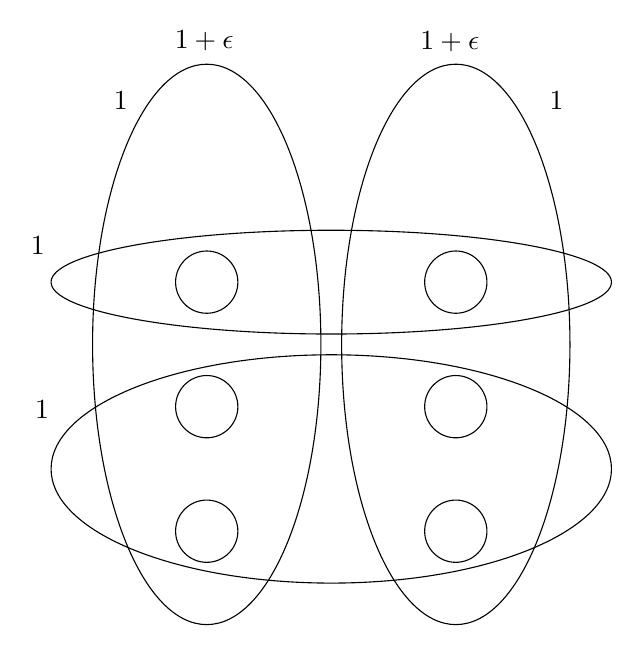
\begin{tikzpicture}[x=0.75pt,y=0.75pt,yscale=-1,xscale=1]
	\draw   (150,155) .. controls (150,80.44) and (174.62,20) .. (205,20) .. controls (235.38,20) and (260,80.44) .. (260,155) .. controls (260,229.56) and (235.38,290) .. (205,290) .. controls (174.62,290) and (150,229.56) .. (150,155) -- cycle ;
	\draw   (190,245) .. controls (190,236.72) and (196.72,230) .. (205,230) .. controls (213.28,230) and (220,236.72) .. (220,245) .. controls (220,253.28) and (213.28,260) .. (205,260) .. controls (196.72,260) and (190,253.28) .. (190,245) -- cycle ;
	\draw   (190,185) .. controls (190,176.72) and (196.72,170) .. (205,170) .. controls (213.28,170) and (220,176.72) .. (220,185) .. controls (220,193.28) and (213.28,200) .. (205,200) .. controls (196.72,200) and (190,193.28) .. (190,185) -- cycle ;
	\draw   (190,125) .. controls (190,116.72) and (196.72,110) .. (205,110) .. controls (213.28,110) and (220,116.72) .. (220,125) .. controls (220,133.28) and (213.28,140) .. (205,140) .. controls (196.72,140) and (190,133.28) .. (190,125) -- cycle ;
	\draw   (270,155) .. controls (270,80.44) and (294.62,20) .. (325,20) .. controls (355.38,20) and (380,80.44) .. (380,155) .. controls (380,229.56) and (355.38,290) .. (325,290) .. controls (294.62,290) and (270,229.56) .. (270,155) -- cycle ;
	\draw   (310,245) .. controls (310,236.72) and (316.72,230) .. (325,230) .. controls (333.28,230) and (340,236.72) .. (340,245) .. controls (340,253.28) and (333.28,260) .. (325,260) .. controls (316.72,260) and (310,253.28) .. (310,245) -- cycle ;
	\draw   (310,185) .. controls (310,176.72) and (316.72,170) .. (325,170) .. controls (333.28,170) and (340,176.72) .. (340,185) .. controls (340,193.28) and (333.28,200) .. (325,200) .. controls (316.72,200) and (310,193.28) .. (310,185) -- cycle ;
	\draw   (310,125) .. controls (310,116.72) and (316.72,110) .. (325,110) .. controls (333.28,110) and (340,116.72) .. (340,125) .. controls (340,133.28) and (333.28,140) .. (325,140) .. controls (316.72,140) and (310,133.28) .. (310,125) -- cycle ;
	\draw   (130,215) .. controls (130,184.62) and (190.44,160) .. (265,160) .. controls (339.56,160) and (400,184.62) .. (400,215) .. controls (400,245.38) and (339.56,270) .. (265,270) .. controls (190.44,270) and (130,245.38) .. (130,215) -- cycle ;
	\draw   (130,125) .. controls (130,111.19) and (190.44,100) .. (265,100) .. controls (339.56,100) and (400,111.19) .. (400,125) .. controls (400,138.81) and (339.56,150) .. (265,150) .. controls (190.44,150) and (130,138.81) .. (130,125) -- cycle ;

	\draw (119,102) node [anchor=north west][inner sep=0.75pt]   [align=left] {$1$};
	\draw (121,181) node [anchor=north west][inner sep=0.75pt]   [align=left] {$1$};
	\draw (159,32) node [anchor=north west][inner sep=0.75pt]   [align=left] {$1$};
	\draw (369,32) node [anchor=north west][inner sep=0.75pt]   [align=left] {$1$};
	\draw (188.33,2.67) node [anchor=north west][inner sep=0.75pt]   [align=left] {$1+\epsilon$};
	\draw (306.67,3) node [anchor=north west][inner sep=0.75pt]   [align=left] {$1+\epsilon$};
\end{tikzpicture}

		\caption{Esempio di input "cattivo" per $n=8$}
		\label{fig:setcover_tightness}
	\end{figure}

	L'algoritmo sceglie nell'ordine gli insiemi $S_i$ in quanto il costo di aggiungerli è, per ogni iterazione $j$, $\frac{1}{n/2^j}$, contro un costo di $\frac{1+\varepsilon}{n/2^j}$ per scegliere $A$ o $B$.
	Questo porta un costo complessivo di $\log_2 n$. La soluzione ottima tuttavia è naturalmente quella composta dagli insiemi $A$ e $B$, che ha un costo di $2+2\varepsilon$. Il rapporto tra le due è necessariamente logaritmico.
\end{proof}



\section{\VertexCover}
Una copertura per un grafo non orientato $G=(V,E)$ è un insieme di vertici $X\subseteq V$ tale che ogni lato di $E$ incide su un vertice in $X$.
Il problema \VertexCover associa a ogni vertice un peso e cerca la copertura di costo complessivo minimo.
\VertexCover è \NPO-completo.

\popt{\VertexCover}
{Grafo non orientato $G=(V,E)$ e pesi $w_1,\dots,w_n$, con $n=\card V$ e $w_i\in\Q^+~\forall i$}
{$X\subseteq V$}
{Determinare una copertura di $G$ di costo minimo}
{$X\subseteq V$ tale che $\forall e\in E ~ e\cap X\neq\emptyset$}
{$\MIN$}
{$w=\sum_{i\in X} w_i$}

Si considerino i problemi di decisione associati a \VertexCover e \MinSetCover.
Un'istanza $\tuple{G=(V,E),\angle{w_i}_{i\in V}}$ di \VertexCover può essere convertita in tempo polinomiale in una di \MinSetCover scegliendo come insiemi gli insiemi dei lati incidenti su ogni vertice $i$:
\begin{equation*}
	S_i=\set{e\in E\mid i\in e}
\end{equation*}
L'insieme universo è $E$ e i pesi sono quelli del vertice relativo a ogni insieme.

\begin{theorem}
	Sia $D$ il grado massimo di un grafo di input a \VertexCover. \VertexCover è $H(D)$-approssimabile.
\end{theorem}


\subsection{\PricedVertexCover}
Si consideri un'istanza di \VertexCover formata dal grafo $G=(V,E)$ e i pesi $\angle{w_i}_{i\in V}$.
$\angle{P_e}_{e\in E}$ è un \emph{assegnamento di prezzi} sui lati.
Un assegnamento $\angle{P_e}_{e\in E}$ si dice \emph{equo} se e solo se
\begin{equation*}
	\forall i\in V\quad\sum_{e\ni i} P_e\leq w_i \text.
\end{equation*}
Un assegnamento si dice \emph{stretto} su un vertice $i$ se e solo se
\begin{equation*}
	\forall i\in V\quad\sum_{e\ni i} P_e = w_i \text.
\end{equation*}

\begin{lemma}\label{lem:vcov_pricing_eq_sum_p_e_w_opt}
	Se $\angle{P_e}_{e\in E}$ è equo allora
	\begin{equation*}
		\sum_{e\in E} P_e \leq w\star
	\end{equation*}
	dove $w\star$ il costo ottimo per l'istanza di \VertexCover.
\end{lemma}
\begin{proof}
	Sia $X\star\subseteq V$ una soluzione ottima. Poiché $\angle{P_e}_{e\in E}$ è equo:
	\begin{equation*}
		\sum_{i\in X\star} \sum_{e\ni i} P_e \leq \sum_{i\in X\star} w_i = w\star \text.
	\end{equation*}
	Ogni lato del grafo incide su un vertice di $X\star$, quindi
	\begin{equation*}
		\sum_{e\in E} P_e \leq \sum_{i\in X\star} \sum_{e\ni i} P_e \leq w\star \text.
	\end{equation*}
\end{proof}

L'algoritmo \ref{algo:PricedVertexCover} usa una tecnica di pricing per costruire una soluzione per \VertexCover.
\begin{algorithm}
	\caption{\PricedVertexCover}
	\label{algo:PricedVertexCover}
	\KwInput{$G=(V,E)$, $\angle{w_i}_{i\in V}$}

\For{$e \in E$}{
	$P_e \asn 0$\;
}
\While{esiste un lato $\bar e=\set{\bar i,\bar j}$ tale che $\angle{P_{\bar e}}$ non è stretto né su $\bar i$ né su $\bar j$}{
	$\Delta \asn \min\set{w_{\bar i}-\sum_{e\ni\bar i} P_e , w_{\bar j}-\sum_{e\ni\bar j} P_e}$\;
	$P_{\bar e} \asn P_{\bar e} + \Delta$\;
}
$S \asn \set{v\in V \mid \angle{P_e} \text{ è stretto su } v}$\;
\Return {$S$}\;

\end{algorithm}

\begin{lemma}\label{lem:pvcov_w_le_w_sum_P_e}
	L'algoritmo \ref{algo:PricedVertexCover} produce una soluzione $S$ ammissibile per \VertexCover. Inoltre al termine dell'esecuzione vale:
	\begin{equation*}
		w \leq 2 \sum_{e \in E} P_e \text.
	\end{equation*}
\end{lemma}
\begin{proof}
	All'uscita dal ciclo, non esistono lati $\set{i,j}$ tali che $\angle{P_e}$ non è stretto né su $i$ né su $j$.
	Quindi l'insieme $S$ dei vertici su cui $\angle{P_e}$ è stretto è una copertura.

	Essendo $S$ una soluzione ammissibile, per definizione:
	\begin{equation*}
		w = \sum_{i\in S} w_i \text.
	\end{equation*}
	Poiché $S$ contiene solo vertici su cui $\angle{P_e}$ è stretto:
	\begin{equation*}
		\forall i\in S \quad w_i = \sum_{e\ni i} P_e \text.
	\end{equation*}
	Ergo
	\begin{equation*}
		w = \sum_{i\in S} \sum_{e\ni i} P_e \text.
	\end{equation*}
	Poiché un lato compare nella somma al più $2$ volte:
	\begin{equation*}
		w \leq 2 \sum_{e\in E} P_e \text.
	\end{equation*}
\end{proof}

\begin{theorem}
	\PricedVertexCover è un algoritmo $2$-approssimante per \VertexCover.
\end{theorem}
\begin{proof}
	\begin{equation*}
		\frac{w}{w\star} \underset{\text{lemma \ref{lem:pvcov_w_le_w_sum_P_e}}}{\leq}
		\frac{2\sum_{e\in E} P_e}{w\star} \underset{\text{lemma \ref{lem:vcov_pricing_eq_sum_p_e_w_opt}}}{\leq}
		\frac{2\sum_{e\in E} P_e}{\sum_{e\in E} P_e} = 2 \text.
	\end{equation*}
\end{proof}


\subsection{\VertexCover tramite arrotondamento di \LinearProgramming}
Si consideri il problema di programmazione lineare e la sua versione vincolata all'integrità della soluzione, il problema di programmazione lineare intera.

\popt{\LinearProgramming}
{Sistema $Ax\geq b$, con $A\in\Q^{m\times n},b\in\Q^m$ ($x$ incognito), vettore $c\in\Q^n$.}
{Assegnamenti per $x$ in $\Q^n$}
{Determinare il vettore $x$ che minimizza la funzione obiettivo}
{$x\in\Q^n\mid Ax\geq b$}
{$\MIN$}
{Funzione obiettivo $c\trans x$}

\popt{\IntegerLinearProgramming}
{Sistema $Ax\geq b$, con $A\in\Q^{m\times n},b\in\Q^m$ ($x$ incognito), vettore $c\in\Q^n$.}
{Assegnamenti per $x$ in $\Z^n$}
{Determinare il vettore $x$ che minimizza la funzione obiettivo}
{$x\in\Z^n\mid Ax\geq b$}
{$\MIN$}
{Funzione obiettivo $c\trans x$}

Per lo stesso input, una soluzione ottima di \IntegerLinearProgramming è ammissibile, ma non necessariamente ottima, per \LinearProgramming.
Viceversa una soluzione ottima per \LinearProgramming può non essere ammissibile per un'istanza di \IntegerLinearProgramming dallo stesso input.

\LinearProgramming è un problema appartenente a \PO (l'ottimo può essere trovato polinomialmente ad esempio con l'algoritmo di Karmarkar \cite{Karmarkar:84:LP}), mentre \IntegerLinearProgramming è \NPO-completo.

Data un'istanza di \VertexCover $\tuple{G=(V,E),\angle{w_i}_{i\in V}}$, con $n:=\card V$ e $m:=\card E$, si consideri l'istanza di \IntegerLinearProgramming in cui il sistema di input è così costruito:
\begin{equation*}
	\begin{cases}
		x_i\geq 0     & \qquad \forall i\in V         \\
		x_i\leq 1     & \qquad \forall i\in V         \\
		x_i+x_j\geq 1 & \qquad \forall \set{i,j}\in E \\
	\end{cases}
\end{equation*}
e la funzione obiettivo è
\begin{equation*}
	w = \min\sum_{i\in V} w_i x_i
\end{equation*}

Una soluzione $x$ dell'istanza di \IntegerLinearProgramming costruita si può interpretare come una soluzione di \VertexCover in cui $x_i=1\iff i\in X$.

Si consideri l'istanza di \LinearProgramming ottenuta rilassando il vincolo di integrità dell'istanza precedente.
Una soluzione ottima $x$ di tale istanza può essere calcolata in tempo polinomiale, ma non è, in generale, ammissibile per la sua versione intera.
Si consideri il vettore $r$, ottenuto dall'arrotondamento di $x$, ossia, per ciascun $i\in n$:
\begin{equation*}
	r_i:= \begin{cases}
		1 & \quad x_i\geq\frac{1}{2} \\
		0 & \quad x_i<\frac{1}{2}
	\end{cases}
\end{equation*}

\begin{lemma}\label{lem:ilp_r_ammiss}
	Il vettore $r$ è una soluzione ammissibile di \IntegerLinearProgramming.
\end{lemma}
\begin{proof}
	Per definizione, $0\leq r\leq 1$. Se non fosse $r_i+r_j\geq 1~\forall \set{i,j}\in E$, siano $\bar i,\bar j$ tali che $r_{\bar i}+r_{\bar j}<1$.
	Allora $r_{\bar i}=r_{\bar j}=0$. Per definizione di $r$ si ha $x_{\bar i}<\frac 12$ e $x_{\bar j}<\frac 12$.
	Ma allora $x_{\bar i}+x_{\bar j}<1$, il che contraddice l'ammissibilità di $x$.
\end{proof}

\begin{lemma}\label{lem:ilp_r_i_leq_2_x_i}
	\begin{equation*}
		\forall i\in V \qquad r_i \leq 2x_i
	\end{equation*}
\end{lemma}
\begin{proof}
	Se $r_i=0$ la disuguaglianza è ovvia;
	se $r_i=1$ allora, $x_i\geq \frac 12$ e $2x_i\geq 1=r_i$.
\end{proof}

\begin{theorem}\label{lem:ilp_appr}
	L'insieme $\set{i\in V\mid r_i=1}$ è una $2$-approssimazione per \VertexCover.
\end{theorem}
\begin{proof}
	Sia $w:=\sum{i\in V} w_i r_i$ il costo della soluzione di \VertexCover indotta dall'istanza arrotondata di \LinearProgramming, e sia $w\star$ la soluzione ottima. Si denoti con $w\star_{\text{LP}}$ il costo ottimo dell'istanza di \LinearProgramming e $w\star_{\text{ILP}}$ quello di \IntegerLinearProgramming.
	Applicando il lemma \ref{lem:ilp_r_i_leq_2_x_i}:
	\begin{equation*}
		w = \sum_{i\in V} w_i r_i \leq 2\sum_{i\in V} w_i x_i = 2w\star_{\text{LP}} \leq 2w\star_{\text{ILP}} = w\star
	\end{equation*}
\end{proof}





\section{\DisjointPaths}
Dato un grafo orientato su cui sono selezionati un numero di vertici \flang{source} e un numero di rispettivi vertici \flang{target} (potenzialmente con molteplicità), il problema \DisjointPaths si pone l'obiettivo di massimizzare il numero di coppie source-target connettibili da un cammino usando ogni arco un numero massimo di $c$ volte, dove $c$ è un dato parametro detto di congestione.
Il problema prende il nome dalla sua variante con $c=1$, in cui i cammini non hanno archi in comune.
\DisjointPaths è \NPO-completo.

\popt{\DisjointPaths}
{Grafo orientato $G=(V,E)$, vertici $\angle{s_i}_{i\in k}$ e $\angle{t_i}_{i\in k}$ e un parametro $c\in\N^+$}
{$I\subseteq k$, cammini $\angle{\pi_i}_{i\in I}$, con $\pi_i:=s_i\leadsto t_i$}
{Determinare il massimo numero di coppie $s_i,t_i$ che si possono connettere con un cammino, usando un arco al più $c$ volte complessivamente}
{$I\subseteq k$, cammini $\angle{\pi_i}_{i\in I}$ tali che nessun arco $e\in E$ appartenga ai cammini più di $c$ volte}
{$\MAX$}
{$\card I$}


\subsection{\PricedDisjointPaths}
L'algoritmo \ref{algo:PricedDisjointPaths} usa una tecnica di pricing in cui viene definita una funzione di costo $l:E\to\Q^+$ per gli archi, estendibile ai cammini $\tuple{x_0,x_1\dots,x_{t-1},x_t}$ con $l(\tuple{x_0,x_1,\dots,x_{t-1},x_t}):=l((x_0,x_1))+\dots+l((x_{t-1},x_t))$.
L'algoritmo fa inoltre uso di un valore $\beta$ che, come si vedrà, può essere calcolato in modo da ottimizzare il risultato.
\SetKwFunction{MinPath}{MinPath}
La procedura \MinPath restituisce, in tempo polinomiale, un cammino di costo minimo e l'indice $i$ dei vertici $s_i$ e $t_i$ che collega, con $i\notin I$. Se un cammino del genere non esiste, la procedura restituisce un cammino vuoto.
L'algoritmo produce una soluzione ammissibile per \DisjointPaths, dal momento che $P$ contiene solo cammini con archi utilizzati al più $c$ volte (dopo $c$ volte un arco viene eliminato) e che collegano, per definizione di \MinPath, vertici non ancora collegati.
\PricedDisjointPaths ha un costo polinomiale: utilizzando ad esempio Floyd-Warshall la procedura \MinPath può essere implementata in $O(\card V^3)$ e viene ripetuta un massimo di $k$ volte, per un costo totale in tempo di $O(k\card V^3)$.

\begin{algorithm}
	\caption{\PricedDisjointPaths}
	\label{algo:PricedDisjointPaths}
	\KwInput{$G=(V,E), \angle{s_i}_{i\in k}, \angle{t_i}_{i\in k}, c\in\N^+, b\in\Q^+$}

$I \asn \emptyset$\;
$P \asn \emptyset$\;
\For{$e\in E$}{
	$l(e) \asn 1$\;
}
\While{true}{
	$\pi,i \asn \MinPath(G,l)$\;
	\If{$\pi=\langle\rangle$}{
		\Return{$I,P$}\;
	}
	$I \asn I\cup\set{i}$\;
	$P \asn P\cup\set{\pi}$\;

	\tcc{Aggiorna i costi ed elimina gli archi già usati $c$ volte}
	\For{$e\in\pi$}{
		$l(e) = l(e) \cdot \beta $\;
		\If{$l(e) = \beta^c$}{
			elimina $e$ \;
		}
	}
}


\end{algorithm}

A una data iterazione dell'algoritmo, un cammino $\pi$ si dice \emph{corto} se e solo se $l(\pi)<\beta^c$.
Un cammino $\pi$ si dice \emph{utile} se e solo se collega una coppia $i\notin I$.

Finché esistono cammini corti e utili, l'algoritmo seleziona uno di essi a ogni iterazione.
Quando nessun cammino è corto e utile, l'esecuzione si ferma oppure iniziano a venire selezionati cammini lunghi (i.e. non corti).
Si consideri la prima iterazione $\bar t$ in cui non esistono cammini corti e utili, o il termine dell'esecuzione se tale iterazione non esiste.
Sia $\bar l$ la funzione di costo in tale iterazione e $\bar I$ l'insieme degli indici dei vertici collegati da cammini.

\begin{lemma}\label{lem:priceddpaths_non_included_non_short}
	Se all'iterazione $\bar t$ la coppia $\tuple{s_i,t_i}$ non è stata collegata dalla soluzione corrente, allora il costo del relativo cammino ottimo $\pi\star_i$ è maggiore o uguale a $\beta^c$:
	\begin{equation*}
		\bar l(\pi\star_i)\geq\beta^c\qquad\forall i\notin I
	\end{equation*}
\end{lemma}
\begin{proof}
	Se fosse $\bar l(\pi\star_i)<\beta^c$, allora $\pi\star$ sarebbe corto e utile, pertanto sarebbe stato selezionato prima dell'iterazione $\bar t$.
\end{proof}

\begin{lemma}\label{lem:priceddpaths_sum_l_a_leq_bc_i_m}
	Sia $m:=\card E$.
	\begin{equation*}
		\sum_{e\in E}\bar l(e) \leq \beta^{c+1}\card{\bar I} + m
	\end{equation*}
\end{lemma}
\begin{proof}~
	\begin{itemize}
		\item Alla prima iterazione, $\sum_{e\in E} l_0(e) = \sum_{e\in E} 1 = m$.
		\item Al termine di ogni iterazione $j<\bar t$, si modificano i valori $l_j$ in valori $l_{j+1}$ così scelti:
		      \begin{equation*}
			      l_{j+1}(e) =
			      \begin{cases}
				      l_j(e)            & \quad\text{se } e\notin\pi_i \\
				      \beta\cdot l_j(e) & \quad\text{se } e\in\pi_i
			      \end{cases}
		      \end{equation*}
		      Si consideri la differenza tra i pesi complessivi all'iterazione $j$ e quelli all'iterazione $j+1$:
		      \begin{align*}
			      \sum_{e\in E} l_{j+1}(e) - \sum_{e\in E} l_j(e) & = \sum_{e\in E} (l_{j+1}(e)-l_j(e))   \\
			                                                      & = \sum_{e\in\pi}(\beta l_j(e)-l_j(e)) \\
			                                                      & = \sum_{e\in\pi} (\beta-1)l_j(e)      \\
			                                                      & \leq \beta\sum_{e\in\pi}l_j(e)
		      \end{align*}
		      Tale valore è al più uguale a $\beta^{c+1}$, essendo il cammino $\pi$ corto perché $j<\bar t$.
	\end{itemize}
	Quindi, all'inizio dell'iterazione $\bar t$, a un costo iniziale di $m$ sono state aggiunte $\card{\bar I}$ variazioni (una per ogni iterazione e quindi aggiunta di cammini a $I$) di al più $\beta^c$ l'una, ergo:
	\begin{equation*}
		\sum_{e\in E} \bar l(e) \leq \beta^{c+1}\card{\bar I}+m \text.
	\end{equation*}
\end{proof}

\begin{corollario}\label{cor:priceddpaths_cor_1}
	\begin{equation*}
		\sum_{i\in I\star\setminus I} \bar l(\pi_i\star) \geq \beta^c \card{I\star\setminus I} \text.
	\end{equation*}
\end{corollario}
\begin{proof}
	Ottenuto dal lemma \ref{lem:priceddpaths_non_included_non_short} sommando per i valori in $I\star\setminus I$.
\end{proof}

\begin{corollario}\label{cor:priceddpaths_cor_2}
	\begin{equation*}
		\sum_{i\in I\star\setminus I} \bar l(\pi\star_i) \leq c(\beta^{c+1}\card{\bar I}+m) \text.
	\end{equation*}
\end{corollario}
\begin{proof}
	\begin{align*}
		\sum_{i\in I\star\setminus I} \bar l(\pi\star_i) & \leq \sum_{i\in I\star} \bar l(\pi\star_i)                                                                                     \\
		                                                 & \leq c \sum_{e\in E} \bar l(e)             &  & \text{ogni arco è usato al più $c$ volte nella soluzione ammissibile $I\star$} \\
		                                                 & \leq c (\beta^{c+1}\card{\bar I}+m)        &  & \text{dal lemma \ref{lem:priceddpaths_sum_l_a_leq_bc_i_m}}
	\end{align*}
\end{proof}

\begin{theorem}\label{thm:priceddpaths_approx}
	\PricedDisjointPaths è un algoritmo $(1+c(\beta+\beta^{-c}m))$-approssimante per \DisjointPaths.
	Se $\beta=m^{\frac{1}{c+1}}$, \PricedDisjointPaths fornisce una $(1+2cm^{\frac{1}{c+1}})$-approssimazione.
\end{theorem}
\begin{proof}
	Sia $I\star$ la soluzione ottima e $I$ la soluzione prodotta da \PricedDisjointPaths.
	\begin{align*}
		\beta^c\card{I\star} & = \beta^c\card{I\star\cap I}+\beta^c\card{I\star\setminus I}                                                                                  \\
		                     & \leq \beta^c\card{I\star\cap I} + \sum_{i\in I\star\setminus I} \bar l(\pi\star_i) &  & \text{per il corollario \ref{cor:priceddpaths_cor_1}} \\
		                     & \leq \beta^c\card I + \sum_{i\in I\star\setminus I} \bar l(\pi\star_i)                                                                        \\
		                     & \leq \beta^c\card I + c(\beta^{c+1}\card{\bar I}+m)                                &  & \text{per il corollario \ref{cor:priceddpaths_cor_2}} \\
		                     & \leq \beta^c\card I + c(\beta^{c+1}\card I+m)                                      &  & \text{essendo $\bar I\subseteq I$} \text.
	\end{align*}
	Dividendo per $\beta^c$:
	\begin{align*}
		\card{I\star} & \leq \card I+c\beta\card I+c\beta^{-c}m                                                   \\
		              & \leq \card I+c\beta\card I+c\beta^{-c}m\card I &  & \text{essendo $\card I\geq 1$} \text.
	\end{align*}
	Dividendo per $\card I$:
	\begin{equation*}
		\frac{\card{I^*}}{\card I} \leq 1+c\beta+c\beta^{-c}m = 1+c(\beta+\beta^{-c}m)
	\end{equation*}
	% TODO: dimostrare in un'appendice
	Questo valore è minimizzato per $\beta=m^{\frac{1}{c+1}}$, ottenendo:
	\begin{align*}
		\frac{\card{I^*}}{\card I} & \leq 1+c\left(m^{\frac{1}{c+1}}+m^{\frac{-c}{c+1}}m\right) \\
		                           & = 1+c\left(m^{\frac{1}{c+1}}+m^{\frac{-c+c+1}{c+1}}\right) \\
		                           & = 1+2cm^{\frac{1}{c+1}}
	\end{align*}
	L'analisi dimostra che le sole prime $\bar t$ iterazioni producono una $(1+2cm^{\frac{1}{c+1}})$-approssimazione. Dal momento che, come mostrato, $\bar I\subseteq I$, l'algoritmo al termine dell'esecuzione produce una soluzione quantomeno non peggiore.
\end{proof}



\section{\TravelingSalesman}
Il problema del commesso viaggiatore, o \TravelingSalesman (problem, abbreviato in TSP), è uno dei problemi più famosi della teoria dei grafi.
Il problema consiste nel trovare un circuito hamiltoniano di costo minimo in un grafo pesato sugli archi.
Dato un grafo non orientato, un \emph{circuito hamiltoniano} è un circuito che passa per ogni vertice del grafo una e una sola volta.
\TravelingSalesman è \NPO-completo.

\popt{\TravelingSalesman}
{Grafo non orientato $G=(V,E)$, pesi $\angle{\delta_e}_{e\in E}$}
{$\pi\subseteq E$ ordinato}
{Determinare il circuito hamiltoniano di minor costo}
{$\pi$ forma un circuito hamiltoniano}
{$\MIN$}
{$\sum_{e\in\pi} \delta_e$}

Con un abuso di notazione useremo $\delta$ per indicare il costo del suo argomento, inteso come la somma dei pesi degli archi che lo compongono.

L'algoritmo di Christofides, che descriveremo a breve, mette insieme una serie di risultati, problemi e algoritmi e trova un'approssimazione della soluzione ottima di \TravelingSalesman. Introduciamo ora tali nozioni.


\subsection{Requisiti}

\subsubsection{Circuiti euleriani}
Dato un grafo non orientato, un \emph{circuito euleriano} è un circuito che include ogni lato del grafo una e una sola volta. Si noti che possono esistere circuiti euleriani che includono un vertice multiple volte.

Il problema di trovare un circuito euleriano in un grafo (o multigrafo) è stato formalizzato da Eulero a partire dal problema dei ponti di Könisberg, che chiedeva se fosse possibile attraversare tutti i ponti della città una volta e tornare al punto di partenza.
Eulero dimostra una condizione necessaria e sufficiente per l'esistenza di un cammino euleriano in un multigrafo:
\begin{theorem}[di Eulero]\label{thm:eulero}
	Un multigrafo ammette un circuito euleriano se e solo se è connesso e tutti i suoi vertici hanno grado pari.
\end{theorem}

Un risultato fondamentale inerente alla parità del grado dei vertici è il lemma delle strette di mano (\flang{handshaking lemma}):
\begin{lemma}[delle strette di mano]\label{lem:handshaking}
	In ogni grafo, il numero di vertici di grado dispari è pari.
\end{lemma}
\begin{proof}
	Dal momento che ogni arco aumenta il grado di due vertici, la somma dei gradi di tutti i vertici è pari. Ma una somma di interi è pari se e solo se il numero di addendi dispari è pari.
\end{proof}

\subsubsection{Il TSP metrico su cricca}\label{subsub:tsp:criccametrica}

\paragraph{Il TSP su cricca} A partire da un'istanza di \TravelingSalesman composta dal grafo $G=(V,E)$ e i pesi $\angle{\delta_e}_{e\in E}$, si consideri l'istanza composta dalla cricca $K=\left(V,\binom V 2\right)$ e dai pesi $\angle{\bar\delta}_{e\in\binom V 2}$ così definiti:
\begin{equation*}
	\bar\delta_e = \begin{cases}
		\delta_e                 & \quad e \in E    \\
		1+\sum_{e\in E} \delta_e & \quad e \notin E
	\end{cases}
\end{equation*}
Trovando la soluzione ottima di \TravelingSalesman su questa istanza, è facile determinare se il circuito hamiltoniano trovato è una soluzione per il grafo originale.
Poiché ogni arco viene percorso al più una volta (altrimenti i vertici verrebbero ripetuti nel circuito), se il costo totale è al più $\sum_{e\in E} \delta_e$ allora nessun arco assente nel grafo originale è stato usato, e la soluzione è ottima anche per l'istanza originale.
Viceversa, se il costo totale è almeno $1+\sum_{e\in E} \delta_e$ allora non è stato possibile trovare un circuito euleriano che non usasse un arco assente nell'istanza originale, e quindi questa non ha soluzione.
Si può quindi semplificare la risoluzione di \TravelingSalesman senza perdita di generalità limitandosi a risolvere il problema nel caso di cricche.

\paragraph{Il TSP metrico} Semplifichiamo ora il problema, imponendo una caratteristica "metrica" alla funzione dei pesi, cioè la disuguaglianza triangolare:
\begin{equation*}
	\forall i,j,k\in V \quad \delta_{\set{i,j}} \leq \delta_{\set{i,k}} + \delta_{\set{k,j}} \text.
\end{equation*}
Come vedremo, solo grazie a questa assunzione è possibile costruire algoritmi approssimanti per \TravelingSalesman.

\subsubsection{L'albero ricoprente minimo}
Dato un grafo non orientato connesso, un albero ricoprente è un sottografo che sia un albero e mantenga tutti i vertici.
Se il grafo è pesato sui lati, un albero ricoprente minimo minimizza la somma dei costi dei lati che mantiene.
\MinimumSpanningTree (MST) è il problema di ottimizzazione che cerca un albero ricoprente minimo in un grafo.
Il problema è risolvibile esattamente in tempo polinomiale, ad esempio dall'algoritmo di Kruskal in tempo $O(m\log n)$.

\popt{\MinimumSpanningTree}
{Grafo connesso $G=(V,E)$, pesi $\angle{\delta_e}_{e\in E}$}
{Albero $T=(V',E')$}
{Trovare un albero ricoprente minimo per $G$}
{$T$ è un albero tale che $V'=V$}
{$\MIN$}
{$\sum_{e\in E'} \delta_e$}

\subsubsection{\MinimumWeightPerfectMatching}
Dato un grafo non orientato con un numero pari di vertici, un \emph{matching perfetto} è un matching (vedi \ref{sec:BiMaxMatching}) che coinvolge tutti i vertici.
In un grafo pesato sugli archi, \MinimumWeightPerfectMatching è il problema di trovare il matching perfetto a costo complessivo minimo.
\MinimumWeightPerfectMatching è risolvibile esattamente in tempo polinomiale, ad esempio con il \flang{blooming algorithm} in tempo $O(m\log n)$.

\popt{\MinimumWeightPerfectMatching}
{Grafo $G=(V,E)$ tale che $\card V$ è pari, pesi $\angle{\delta_e}_{e\in E}$}
{Matching $M\subseteq E$}
{Determinare un matching perfetto di costo minimo}
{$M$ è un matching perfetto su $G$}
{$\MIN$}
{$\sum_{e\in M} \delta_e$}


\subsection{L'algoritmo di Christofides}
L'algoritmo di Christofides per TSP metrico su cricca applica i concetti precedentemente descritti manipolando diverse strutture fino a ottenere un cammino hamiltoniano. Ricevendo in input una cricca $G=(V,E)$ e pesi $\angle{\delta_e}_{e\in E}$, i passi dell'algoritmo sono i seguenti:
\begin{enumerate}
	\item identificare un albero ricoprente minimo $T$ per $G$;
	\item sia $D$ il grafo indotto su $G$ dall'insieme dei suoi vertici che hanno grado dispari in $T$.
	      Questi sono in numero pari per il lemma \ref{lem:handshaking}. È quindi possibile identificare un matching perfetto minimo $M$ su $D$;
	\item sia $H$ il multigrafo indotto su $G$ dall'unione disgiunta dei lati di $T$ ed $M$. In $H$ tutti i vertici hanno grado pari, poiché quelli che avevano grado dispari in $T$ hanno un nuovo arco grazie a $M$. In virtù del lemma \ref{thm:eulero} si può trovare un circuito euleriano $\pi$ in $H$;
	\item trasformare il circuito euleriano $\pi$, valido anche per $G$, in un hamiltoniano $\tilde\pi$.
	      Ogni volta che $\pi$ passa su un vertice $v$ una seconda volta tramite i lati $\set{a,v}$ e $\set{v,b}$, è sufficiente "saltare" tale vertice sostituendo in $\tilde\pi$ i due lati con il lato $\set{a,b}$ (esistente in quanto si sta lavorando sulla cricca originale), con conseguente diminuzione del costo in virtù della disuguaglianza triangolare.
\end{enumerate}

L'analisi dell'algoritmo ci porta a dimostrare un risultato di approssimazione rispetto al TSP metrico su cricca.
\begin{lemma}\label{lem:chri_spanning}
	In una cricca $G$ pesata metricamente sui lati, il costo $\delta(T)$ di un albero ricoprente minimo $T$ non è peggiore del costo minimo $\delta\star$ di un cammino hamiltoniano su $G$:
	\begin{equation*}
		\delta(T) \leq \delta\star
	\end{equation*}
\end{lemma}
\begin{proof}
	Sia $\pi\star$ un circuito hamiltoniano ottimo e sia $e\in\pi\star$.
	Il grafo indotto da $\pi\star\setminus e$ è un albero ricoprente. Pertanto:
	\begin{equation*}
		\delta(T) \leq \delta(\pi\star\setminus e) \leq\delta\star \text.
	\end{equation*}
\end{proof}

\begin{lemma}\label{lem:chri_matching}
	\begin{equation*}
		\delta(M) \leq \frac 1 2 \delta\star
	\end{equation*}
\end{lemma}
\begin{proof}
	Si consideri un circuito hamiltoniano ottimo $\pi\star$. Poiché è hamiltoniano, questo comprende i vertici di $D$. Cortocircuitando $\pi\star$ sui soli vertici di $D$, si ottiene un circuito di peso complessivo minore o uguale a quello di $\pi\star$ (per la disuguaglianza triangolare) e che ha un numero di lati pari (poiché i vertici di $D$ sono pari). Alternando i lati di questo circuito, si formano due matching $M_1$ e $M_2$ perfetti su $D$. Ma poiché $M$ è il matching perfetto di costo minimo per $D$, vale:
	\begin{equation*}
		\delta(\pi\star)\geq\delta(M_1)+\delta(M_2)\geq 2\delta(M) \text. \qedhere
	\end{equation*}
\end{proof}

\begin{theorem}
	L'algoritmo di Christofides è $\frac 3 2$-approssimante per il TSP metrico su cricca.
\end{theorem}
\begin{proof}
	Per la costruzione del circuito hamiltoniano $\tilde\pi$ a partire dal circuito euleriano $\pi$ e grazie ai lemmi sopra dimostrati:
	\begin{equation*}
		\delta(\tilde\pi)\leq\delta(\pi) = \delta(T)+\delta(M)\leq
		\underbrace{\delta\star}_{\text{lemma \ref{lem:chri_matching}}} + \underbrace{\frac{\delta\star}{2}}_{\text{lemma \ref{lem:chri_spanning}}} =
		\frac 3 2 \delta\star \text.
	\end{equation*}
\end{proof}

\begin{theorem}
	Per ogni $\varepsilon>0$ esiste un input del TSP metrico su cricca su cui l'algoritmo di Christofides produce una soluzione $\pi$ tale che
	\begin{equation*}
		\frac 3 2-\varepsilon \leq \frac{\delta(\pi)}{\delta\star}
	\end{equation*}
\end{theorem}
\begin{proof}
	Dato $n$ pari e $\varepsilon\in(0,1)$, si consideri il grafo in figura \ref{fig:christotight}, in cui gli archi sono etichettati con i loro pesi. Si estenda il grafo a una cricca $G$, in cui ogni lato $\set{u,v}$ non rappresentato ha come peso il peso del cammino minimo tra $u$ e $v$ sul grafo originale.

	\begin{figure}[ht]
		\centering
		\begin{tikzpicture}[vert/.style={minimum size=15pt,draw,circle}]
	\node[vert]		(1) {$v_1$};
	\node[vert,right=of 1]	(2) {$v_2$};
	\node[vert,right=of 2]	(3) {$v_3$};
	\node[vert,right=of 3]	(4) {$v_4$};
	\node[vert,right=of 4]	(5) {$v_{n-2}$};
	\node[vert,right=of 5]	(6) {$v_{n-1}$};
	\node[vert,right=of 6]	(7) {$v_{n}$};

	\draw (1) to node [auto] {$1$} (2);
	\draw (2) to node [auto] {$1$} (3);
	\draw (3) to node [auto] {$1$} (4);
	\draw (5) to node [auto] {$1$} (6);
	\draw (6) to node [auto] {$1$} (7);

	\draw[dotted]		(4) to (5);

	\draw[bend right=40]	(1) to node	[below]	{$1+\epsilon$} (3);
	\draw[bend left=41]	(2) to node	[auto]	{$1+\epsilon$} (4);
	\draw[bend left=37]	(5) to node	[auto]	{$1+\epsilon$} (7);
	\draw[bend right=30]	(3) edge node	[below]	{$1+\epsilon$} (5.5,-1);
	\draw[bend left=30]	(6) edge node	[auto]	{$1+\epsilon$} (7.5,-1);
\end{tikzpicture}

		\caption{Esempio di input "cattivo" per l'algoritmo di Christofides.}
		\label{fig:christotight}
	\end{figure}

	L'algoritmo di Christofides identifica l'albero ricoprente $T$ indotto da tutti i lati di peso $1$, quindi $\delta(T)=n-1$.
	L'algoritmo seleziona poi $D=\set{v_1,v_n}$ e su di esso il matching $M$ composto dal solo lato $\set{v_1,v_n}$ di peso $\delta(M)=(1+\varepsilon)\left(\frac n2-1\right)+1$.
	Sul grafo indotto dall'unione $H$ di $T$ e $M$ l'algoritmo costruisce il circuito euleriano, nonché hamiltoniano, composto dall'unione degli archi di peso $1$ e l'arco che compone $M$.
	Il costo $\delta$ del circuito costruito è quindi:
	\begin{equation*}
		\delta = n-1 + (1+\varepsilon)\left(\frac n2-1\right)+1 = \frac32n+\varepsilon\left(\frac n2-1\right)-1 \text.
	\end{equation*}
	Ma il circuito hamiltoniano ottimo è quello che, a partire da $v_1$, percorre tutti gli archi di peso $1+\varepsilon$ che uniscono vertici di indice dispari, l'arco $\set{v_{n-1},v_n}$, tutti gli archi di peso $1+\varepsilon$ di indice pari e infine l'arco $\set{v_1,v_2}$.
	Il costo $\delta\star$ di tale circuito è:
	\begin{equation*}
		\delta\star = 2(1+\varepsilon)\left(\frac n2-1\right) + 2 = n+\varepsilon(n-2) \text.
	\end{equation*}
	Quindi
	\begin{equation*}
		\frac{\delta}{\delta\star} = \frac{\frac32n+\varepsilon\left(\frac n2-1\right)-1}{n+\varepsilon(n-2)}
	\end{equation*}
	Che è definitivamente\footnote{Precisamente, la disequazione è vera per $n\geq 2+\frac{1-2\varepsilon}{\varepsilon^2}$.} maggiore o uguale a $\frac 3 2-\varepsilon$.

\end{proof}


\subsection{Inapprossimabilità di \TravelingSalesman}
Abbandonando l'ipotesi di disuguaglianza triangolare della funzione $\delta$, il problema \TravelingSalesman è inapprossimabile.
Al fine di dimostrare ciò ricordiamo che decidere se un grafo contiene un cammino hamiltoniano è un problema \NP-completo.

\begin{theorem}
	Se $\P\neq\NP$, non esiste alcun $\alpha>1$ tale che \TravelingSalesman sia $\alpha$-approssimabile.
\end{theorem}
\begin{proof}
	Fissato $\alpha>1$, sia $G=(V,E)$ un grafo non orientato in cui tutti i lati hanno peso $1$.
	Sia $G'$ la sua estensione a cricca, ottenuta con il metodo citato nel paragrafo \ref{subsub:tsp:criccametrica}, ossia in cui la funzione peso $\delta$ è così definita:
	\begin{equation*}
		\delta(x,y) = \begin{cases}
			1          & \quad \set{x,y}\in E    \\
			\alpha n+1 & \quad \set{x,y}\notin E
		\end{cases}
	\end{equation*}
	Se $G$ ammette un circuito hamiltoniano, allora tale circuito è ammesso anche in $G'$ e ha costo $n<\alpha n$.
	Viceversa, se $G$ non ammette un circuito hamiltoniano allora ogni circuito hamiltoniano in $G'$ ha costo di almeno $\alpha n+1$.

	Se esiste un algoritmo $\alpha$-approssimante per \TravelingSalesman, questo trova in tempo polinomiale un circuito hamiltoniano in $G'$ di costo al più $\alpha n$. Ma un tale circuito esiste se e solo se esiste un cammino hamiltoniano in $G$. L'algoritmo decide quindi in tempo polinomiale se un grafo $G$ ammette un cammino hamiltoniano, il che è impossibile se $\P\neq\NP$.
\end{proof}



\section{\texorpdfstring{$2$}{2}-\LoadBalancing}
$2$-\LoadBalancing è una specializzazione di \LoadBalancing in cui il numero di macchine $m$ è uguale a $2$.
Questo problema è anche chiamato \MinimumPartition in quanto è equivalente al bilanciare una partizione insiemistica di due elementi.
Il problema è \NPO-completo.

L'algoritmo \ref{algo:partitionbalance} è un algoritmo \PTAS-caratterizzante per $2$-\LoadBalancing.
L'algoritmo opera in tempo polinomiale rispetto alla dimensione dell'input ed esponenziale rispetto a $\varepsilon$.

\begin{algorithm}
	\caption{Algoritmo \PTAS per $2$-\LoadBalancing.}
	\label{algo:partitionbalance}
	\KwInput{$m_1,m_2,t_1,\dots,t_n,\varepsilon$}

\If{$\epsilon\geq 1$}{
	assegna i task $\set{t_1,\dots,t_n}$\;
	\Return\;
}
Ordina in ordine decrescente di costo i task $t_1,\dots,t_n$\;
$k \asn \ceil{\frac{1}{\epsilon}-1}$\;
Cerca esaustivamente l'assegnamento ottimo dei task $t_1,\dots,t_k$ e applicalo\;
Assegna in modo greedy (i.e. alla macchina più scarica) i task $t_{k+1},\dots,t_n$\;

\end{algorithm}

\begin{theorem}
	Dato $\varepsilon>0$, l'algoritmo \ref{algo:partitionbalance} produce in tempo polinomiale in $n$ una $(1+\varepsilon)$-approssimazione per $2$-\LoadBalancing.
\end{theorem}
\begin{proof}
	Sia $L:=\frac12\sum_{i=1}^n t_i$.
	Il costo ottimo è almeno $L$, perciò se $\varepsilon\geq1$, assegnando tutti i task alla stessa macchina si ottiene un costo di $\sum_{i=1}^n t_i=2L\leq(1+\varepsilon)L\star$. Qualunque altro assegnamento produrrebbe una soluzione migliore, e quindi altrettanto buona, per questo caso.

	Se $\varepsilon<1$, si consideri lo stato delle macchine al termine dell'esecuzione e sia $L_1\geq L_2$ senza perdita di generalità.
	Sia $t_h$ l'ultimo task assegnato alla macchina $1$.
	\begin{itemize}
		% TODO: inserire considerazioni della dispensa aggiuntiva del prof
		\item Se $h\leq k$, $t_h$ è stato assegnato nella fase esaustiva e pertanto la soluzione costruita è ottima.
		\item Se $h>k$, allora $t_h$ è assegnato nella fase greedy, quindi, se $L_2'$ è il carico della macchina $2$ all'assegnamento di $t_h$, vale:
		      \begin{equation*}
			      L_1-t_h\leq L_2'\leq L_2
		      \end{equation*}
		      Quindi, ricordando che $L_1+L_2=2L$:
		      \begin{align}
			      L_1-t_h  & \leq L_2 \nonumber                    \\
			      2L_1-t_h & \leq L \nonumber                      \\
			      L_1      & \leq L+\frac{t_h}{2} \label{eq:2lb:1}
		      \end{align}
		      Inoltre vale
		      \begin{equation}\label{eq:2lb:2}
			      2L = \underbrace{t_0+t_1+\dots+t_k}_{\geq t_hk}+\underbrace{\dots+t_h+\dots+t_{n-1}}_{\geq t_h} \geq t_h(k+1)
		      \end{equation}
		      Ergo:
		      \begin{align*}
			      \frac{L_1}{L\star} & \leq \frac{L+\frac{t_h}{2}}{L\star}        &  & \text{per la \ref{eq:2lb:1}} \\
			                         & \leq \frac{L+\frac{t_h}{2}}{L}             &  & L\star\geq L                 \\
			                         & = 1+\frac{t_h}{2L}                                                           \\
			                         & \leq 1+\frac{t_h}{t_h(k+1)}                &  & \text{per la \ref{eq:2lb:2}} \\
			                         & = 1+\frac{1}{k+1}                                                            \\
			                         & \leq 1+\frac{1}{\frac{1}{\varepsilon}-1+1} &  & k\geq\frac{1}{\varepsilon}-1 \\
			                         & = \varepsilon+1 \text.
		      \end{align*}
	\end{itemize}
	Considerate le complessità delle operazioni di ordinamento, della ricerca esaustiva delle $2^k$ combinazioni per la parte ottima, e della coda per la parte greedy, l'algoritmo ha tempo d'esecuzione $O(n\log n+2^{\frac{1}{\varepsilon}}n)$.
\end{proof}



\section{\Knapsack}
\Knapsack, il problema dello zaino, è un celebre problema di ottimizzazione.
Dati uno zaino di capacità $W$ e degli oggetti, ciascuno con un valore e un volume (o peso), il problema consiste nel selezionare un gruppo di oggetti in modo che il loro volume non ecceda la capacità dello zaino ma il loro valore complessivo sia massimo.
\Knapsack è un problema \NPO-completo.

% TODO: bisogna pensare a un modo furbo di indicizzare gli oggetti di modo che la colonna i gestisca l'oggetto di indice i. Occhio però alla notazione angle, che non supporta facilmente gli indici da 1
\popt{\Knapsack}
{$n$ oggetti con valori $\angle{v_i}_{i\in n}\in\N^+$ e pesi $\angle{w_i}_{i\in n}\in\N^+$, capacità $W\in N$}
{$I\subseteq n$}
{Determinare l'insieme di oggetti di valore complessivo maggiore il cui peso complessivo non superi $W$}
{$\sum_{i\in I}w_i\leq W$}
{$\MAX$}
{$\sum_{i\in I} v_i$}


\subsection{\DynamicKnapsack}
Il problema può essere risolto in modo esatto dall'algoritmo \DynamicKnapsack, basato su programmazione dinamica.
L'algoritmo costruisce una matrice in cui costruisce le soluzioni ottime per istanze di complessità minore di quella in input, usandole per calcolare la soluzione ottima complessiva.

L'elemento $A[i,w]$ della matrice $A\in{\N^+}^{(n+1)\times (W+1)}$ è associato semanticamente al massimo valore ottenibile con i primi $i$ oggetti con una capacità massima di $w$.
Gli elementi $A[0,w]$, per ogni $w\in W+1$, sono vincolati al valore $0$ dal momento che nessun oggetto può essere utilizzato, mentre i restanti valori sono così calcolati:
\begin{equation*}
	A[i+1,w] =
	\begin{cases}
		A[i,w]                       & \quad w_i>w     \\
		\max(A[i,w], A[i,w-w_i]+v_i) & \quad w_i\leq w
	\end{cases}
\end{equation*}
L'algoritmo valuta quindi se l'oggetto $i+1$ ha volume compatibile con la capacità massima: in caso negativo reitera la soluzione che non usa l'ultimo oggetto, in caso positivo sceglie la migliore tra tale soluzione e quella che fa uso dell'ultimo oggetto (costruita aggiungendolo alla soluzione ottima dell'istanza con capacità $w-w_i$).

Riempita la tabella, l'algoritmo può ricostruire la soluzione che produce il valore ottimo $A[n,W]$.
L'algoritmo opera in tempo pseudopolinomiale, in quanto opera su una matrice di dimensione lineare nel valore di $W$, che è esponenziale nella lunghezza dell'input.


\subsection{\WeightDynamicKnapsack}
Una variante dell'algoritmo \DynamicKnapsack costruisce una matrice $B\in{\N^+}^{(n+1)\times (\sum_{i\in n} v_i)}$ in cui l'elemento $B[i,v]$ rappresenta il minimo peso necessario per raggiungere un valore di $v$ usando i primi $i$ oggetti.

L'elemento $B[0,0]$ è posto uguale a $0$. Gli elementi $B[0,v]$, per ogni $v\in\sum_{i\in n} v_i$, sono vincolati al valore $+\infty$ dal momento che il valore $v$ è irraggiungibile. I restanti valori sono così calcolati:
\begin{equation*}
	B[i+1,v] = \min(B[i,v], w_i+B[i,\max(v-v_i,0)])
\end{equation*}
L'algoritmo sceglie quindi la migliore soluzione tra quella che non fa uso dell'oggetto $i+1$-esimo e quella che lo aggiunge alla soluzione che utilizza i primi $i$.

Un algoritmo che usa questa matrice può trovare la soluzione ottima cercando sulla riga $n$ la colonna di indice massimo il cui valore non supera $W$. Un tale algoritmo sarebbe tuttavia poco efficiente per via dell'utilizzo di una matrice con un tale numero di colonne.

L'algoritmo può essere migliorato, a costo di perdere l'esattezza, introducendo una normalizzazione che ridimensiona i valori in base al valore massimo $v_{\max}$.
L'algoritmo risultante approssima a piacere in tempo polinomiale.

Sia $\pi=\tuple{\angle{v_i}_{i\in n},\angle{w_i}_{i\in n},W}$ un'istanza di \Knapsack. Si rimuovano eventuali pesi $i$ tali che $w_i>W$, che non contribuiscono ad alcuna soluzione ammissibile.
Dato un valore $\varepsilon\in(0,1]$, si definisce il valore di scala $\theta$ come
\begin{equation*}
	\theta:=\frac{\varepsilon v_{\max}}{2n} \text.
\end{equation*}
Si considerino le istanze $\bar\pi:=\tuple{\angle{\bar v_i=\ceil{\frac{v_i}{\theta}}\theta}_{i\in n},\angle{w_i}_{i\in n},W}$ e $\hat\pi:=\tuple{\angle{\hat v_i=\ceil{\frac{v_i}{\theta}}}_{i\in n},\angle{w_i}_{i\in n},W}$, che scalano in modo diverso i valori e lasciano invariati pesi e capacità.
Siano $\bar I\star$ e $\hat I\star$ le rispettive soluzioni ottime e $\bar v\star$ e $\hat v\star$ i loro valori.

\begin{lemma}\label{lem:knap_barhat}
	$\bar I\star = \hat I\star \land \bar v\star = \theta\hat v\star$.
\end{lemma}
\begin{proof}
	La funzione obiettivo del problema $\bar\pi$ non è altro che una dilatazione di fattore $\theta$ di quella del problema $\hat\pi$, pertanto le soluzioni ottime sono le stesse e i valori ottimi subiscono una dilatazione.
\end{proof}

\begin{lemma}
	Sia $I$ una soluzione ammissibile per $\pi$. Allora
	\begin{equation*}
		(1+\varepsilon)\sum_{i\in\hat I\star} v_i \geq \sum_{i\in I} v_i
	\end{equation*}
\end{lemma}
\begin{proof}
	\begin{align*}
		\sum_{i\in I} v_i & \leq \sum_{i\in I} \bar v_i                                          &  & \quad \text{arrotondamento per eccesso}      \\
		                  & \leq \sum_{ i\in\bar I\star} \bar v_i                                                                                  \\
		                  & = \sum_{ i\in\hat I\star} \bar v_i                                   &  & \quad \text{per lemma \ref{lem:knap_barhat}} \\
		                  & \leq \sum_{i\in\hat I\star} (v_i+\theta)                             &  & \quad \text{in quanto
		$\bar v_i=\ceil{\frac{v_i}{\theta}}\theta\leq\left(\frac{v_i}{\theta}+1\right)\theta=v_i+\theta$}                                          \\
		                  & \leq n\theta+\sum_{i\in\hat I\star} v_i                                                                                \\
		                  & = \frac{\varepsilon v_{\max}}{2} + \sum_{i\in\hat I\star} v_i \text.
	\end{align*}
	Quindi
	\begin{equation}\label{eq:knap:1}
		\sum_{i\in I} v_i \leq \frac{\varepsilon v_{\max}}{2} + \sum_{i\in\hat I\star} v_i
	\end{equation}

	\noindent Si consideri la soluzione ammissibile composta da un solo peso di valore massimo. Applicando (\ref{eq:knap:1}):
	\begin{gather}
		v_{\max} \leq \frac{\varepsilon v_{\max}}{2} + \sum_{i\in\hat I\star} v_i \leq \frac{v_{\max}}{2} + \sum_{i\in\hat I\star} v_i \nonumber \\
		\sum_{i\in\hat I\star} v_i \geq \frac{v_{\max}}{2} \label{eq:knap:2}
	\end{gather}
	Tornando alla generica soluzione ammissibile $I$ e applicando (\ref{eq:knap:1}) e (\ref{eq:knap:2}):
	\begin{gather*}
		\sum_{i\in I} v_i \leq \frac{\varepsilon v_{\max}}{2} + \sum_{i\in\hat I\star} v_i
		\leq \varepsilon\sum_{i\in\hat I\star} v_i + \sum_{i\in\hat I\star} v_i = (1+\varepsilon)\sum_{i\in\hat I\star} v_i
	\end{gather*}
\end{proof}
\begin{corollario}\label{corol:knapapprox}
	$\displaystyle(1+\varepsilon)\sum_{i\in\hat I\star} v_i \geq v\star$
\end{corollario}

\begin{theorem}
	$\Knapsack\in\FPTAS$.
\end{theorem}
\begin{proof}
	Risolvendo il problema $\hat\pi$ ottimamente con $\WeightDynamicKnapsack$ si trova una soluzione $\hat I\star$ che ha valore, nella funzione obiettivo originale, di $\sum_{i\in\hat I\star} v_i$. In virtù del corollario \ref{corol:knapapprox} tale valore produce un rapporto di approssimazione di $1+\varepsilon$.

	Per verificare che questo metodo sia effettivamente polinomiale in $n$ e $\frac{1}{\varepsilon}$, valutiamo il numero di colonne della matrice $B$.
	Nel caso peggiore tutti i pesi sono uguali a $\hat v_{\max}$, pertanto esso sarà $n \hat v_{\max}$.
	Ma vale
	\begin{equation*}
		\hat v_{\max}=\ceil{\frac{v_{\max}}{\theta}}=\ceil{\frac{2nv_{\max}}{\varepsilon v_{\max}}}=\ceil{\frac{2n}{\varepsilon}}\leq\frac{2n}{\varepsilon}+1 \text,
	\end{equation*}
	quindi la dimensione complessiva della matrice è
	\begin{equation*}
		n\cdot n\hat v_{\max}\leq n^2\left(\frac{2n}{\varepsilon}+1\right)=\frac{2n^3}{\varepsilon}+n^2
	\end{equation*}
\end{proof}

Non si può applicare alla variante originale di \DynamicKnapsack un approccio analogo a quello sopra descritto, in quanto la compressione porterebbe a un'approssimazione, invece che nei valori, nei pesi, perdendo quindi la garanzia di ammissibilità delle soluzioni ottenute.

\chapter{Algoritmi probabilistici}
Il modello di calcolo di riferimento per gli algoritmi deterministici, inclusi quelli approssimanti visti fin'ora, è quello della macchina di Turing, in cui a un input corrisponde un output (\cref{fig:mdtdet}).
\begin{figure}[ht]
	\centering
	\begin{tikzpicture}
	\node[draw, rounded corners=5pt, minimum width=2.5cm, minimum height=1.5cm] (tm) {Macchina di Turing};
	\draw[-arr] (-4,0) -- (tm.west)	node[midway,above] {input};
	\draw[-arr] (tm.east) -- (4,0)	node[midway,above] {output};
\end{tikzpicture}

	\caption{Macchina di Turing deterministica}
	\label{fig:mdtdet}
\end{figure}

Un diverso modello di calcolo è quello della macchina di Turing probabilistica (\cref{fig:mdtprob}), che ha accesso a una sorgente aleatoria, cioè un input secondario di bit casuali.

\begin{figure}[ht]
	\centering
	\begin{tikzpicture}
	\node[draw, rounded corners=5pt, minimum width=2.5cm, minimum height=1.5cm] (tm) {Macchina di Turing};
	\draw[-arr] (-4,0) -- (tm.west)	node[midway,above] {input};
	\draw[-arr] (tm.east) -- (4,0)	node[midway,above] {output};
	\matrix (tape) [tape,above=1 of tm] { 0 & 1 & 0 & 1 & 1 & 1 & 0 & 0 & 1 & 1 & 1 & 1 & 1 & 1 & 0 & 0 & \dots\\};
	\draw[-arr,shorten <=-3.5pt] (tape.south) -- (tm.north);
	\node[above=0 of tape] {sorgente aleatoria};
\end{tikzpicture}

	\caption{Macchina di Turing probabilistica}
	\label{fig:mdtprob}
\end{figure}

Un algoritmo basato su questo modello si dice probabilistico, in quanto l'output dipende dall'input e dal seme casuale.
L'algoritmo possiede quindi una distribuzione associata, che mappa un input $x$ alla probabilità di ottenere l'output $y$:
\begin{equation*}
	P(Y = y \mid X = x)
\end{equation*}
Gli algoritmi probabilistici possono risolvere problemi di ottimizzazione quanto di decisione e si dividono in due famiglie:
\begin{description}
	\item[Monte Carlo] la correttezza dell'output, cioè la giusta decisione per i problemi di decisione e il calcolo della soluzione ottima per i problemi di ottimizzazione, è probabilistica; il tempo di esecuzione è deterministico;
	\item[Las Vegas] l'output è deterministicamente corretto; il tempo di esecuzione è probabilistico.
\end{description}
È possibile combinare algoritmi approssimanti con algoritmi probabilistici ottenendo algoritmi che approssimano entro una certa soglia dall'ottimo con una certa probabilità.



\section{\MinCut}
\MinCut è il problema di determinare il taglio minimo in un grafo non orientato.
In un grafo non orientato $G=(V,E)$, un taglio è dato dalla partizione di $V$ in due sottoinsiemi $X, X\compl$.
Il costo del taglio è dato dal numero di archi da vertici in $X$ a vertici in $X\compl$.
\MinCut è \NPO-completo.

\popt{\MinCut}
{Grafo non orientato $G=(V,E)$}
{Taglio $X\subseteq V$}
{Determinare il taglio minimo in $G$}
{$X\subset V\mid X\neq\emptyset$}
{$\MIN$}
{$\card{\set{e\in E\mid e\cap X\neq\emptyset\land e\setminus X\neq\emptyset}}$}

\noindent\MinCut è un problema \NPO-completo.


\subsection{L'algoritmo di Karger}
L'algoritmo di Karger è un algoritmo Monte Carlo per il taglio minimo e si basa sull'operazione di contrazione.
Sia $G=(V,E)$ un multigrafo\footnote{Nei multigrafi sono ammessi lati paralleli, cioè più lati che incidono sulla stessa coppia di vertici. Consideriamo quindi $E$ un insieme dotato di molteplicità. Formalmente, all'insieme è associata una funzione che indica la molteplicità di ogni elemento. Useremo comunque per semplicità le nozioni insiemistiche per insiemi standard.} di input. Si consideri il multigrafo $G'=(V',E')$, dove:
\begin{itemize}
	\item $V':=\set{\bar v\mid v\in V}$, dove $\bar v:=\set{v}$;
	\item $E':=\set{\set{\bar u,\bar v}\mid \set{u,v}\in E}$.
\end{itemize}
La contrazione $G'\downarrow e$ del lato $e=\set{\bar u,\bar v}$ (\cref{fig:contrazione}) consiste in una modifica di $V'$ e $E'$ come segue:
\begin{enumerate}
	\item viene aggiunto a $V'$ un nuovo supervertice $\bar z=\bar u\cup\bar v$;
	\item ogni arco $\set{\bar u,\bar w}\in E'$, con $w\neq v$, è sostituito da un arco $\set{\bar z,\bar w}$;
	\item ogni arco $\set{\bar w,\bar v}\in E'$, con $w\neq u$, è sostituito da un arco $\set{\bar w,\bar z}$;
	\item gli archi del tipo $\set{\bar u,\bar v}$ vengono rimossi da $E'$;
	\item i vertici $\bar u,\bar v$ vengono rimossi da $V'$.
\end{enumerate}

% TODO: questa immagine andrebbe arricchita un po': non fa capire come si fondono gli archi
\begin{figure}[ht]
	\centering
	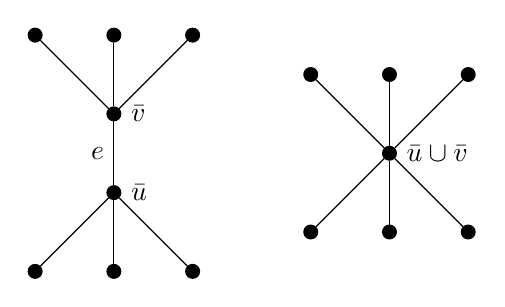
\begin{tikzpicture}[vertex/.style={draw,inner sep=0pt,minimum size=5pt,fill, circle}]
	\node[vertex] at (0, 2)  (u1) {};
	\node[vertex] at (-1, 2)  (u2) {};
	\node[vertex] at (1, 2)  (u3) {};
	\node[vertex,label={0:{$\bar u$}}] at (0, 0)  (a) {};
	\node[vertex,label={0:{$\bar v$}}] at (0, 1)  (b) {};
	\node[vertex] at (0, -1)  (l1) {};
	\node[vertex] at (-1, -1)  (l2) {};
	\node[vertex] at (1, -1)  (l3) {};
	\draw (u1) -- (b);
	\draw (u2) -- (b);
	\draw (u3) -- (b);
	\draw (l1) -- (a);
	\draw (l2) -- (a);
	\draw (l3) -- (a);
	\node at (1.75,0.5) (to) {$\implies$};
	\draw (a) edge node [left] {$e$} (b);
	\node[vertex] at (3.5, 1.5)  (lu1) {};
	\node[vertex] at (2.5, 1.5)  (lu2) {};
	\node[vertex] at (4.5, 1.5)  (lu3) {};
	\node[vertex,label={0:{$\bar u\cup \bar v$}}] at (3.5, 0.5)  (la) {};
	\node[vertex] at (3.5, -0.5)  (ll1) {};
	\node[vertex] at (2.5, -0.5)  (ll2) {};
	\node[vertex] at (4.5, -0.5)  (ll3) {};
	\draw (lu1) -- (la);
	\draw (lu2) -- (la);
	\draw (lu3) -- (la);
	\draw (ll1) -- (la);
	\draw (ll2) -- (la);
	\draw (ll3) -- (la);
\end{tikzpicture}

	\caption{Contrazione $G'\downarrow e$.}
	\label{fig:contrazione}
\end{figure}

In seguito chiameremo semplicemente $G$ il grafo $G'$ derivante dall'input. L'algoritmo \ref{algo:Karger} di Karger effettua contrazioni casuali a partire dal grafo $G$, ottenendo multigrafi $G_0,G_1,\dots$.

\begin{algorithm}[ht]
	\caption{Algoritmo di Karger per \MinCut}
	\label{algo:Karger}
	\SetKwFunction{Unif}{uniformExtraction}
\SetKwFunction{Connected}{isConnected}
\SetKwFunction{FindConnected}{findConnectedComponent}
\SetKwFunction{Choose}{chooseAnElement}
\KwInput{grafo $G=(V,E)$}

\If{$\lnot$\Connected{$G$}}{
	\Return{\FindConnected{$G$}}\;
}
\While{$\card V > 2$}{
	\tcp{Estrai uniformemente a caso un lato e contrailo}
	$e = \Unif{$E$}$\;
	$G = G\downarrow e$\;
}
\tcp{Restituisci uno dei due vertici rimanenti}
\Return{\Choose{$V$}}\;

\end{algorithm}

Chiaramente, l'output dipende dalle scelte dei lati da contrarre, che sono casuali.
Sia $S\star$ il taglio minimo, $k\star$ il numero di lati tagliati da $S\star$ e $G_0,\dots,G_i,\dots$ la sequenza di grafi ottenuti per ogni contrazione operata dall'algoritmo, dove $G_i$ è ottenuto dopo $i$ passi. Si verificano i seguenti fatti:
\begin{oss}\label{oss:kargercontraction}
	\begin{equation*}
		\forall i \quad \card{V_i} = n-i \land \card{E_i} \leq m-i
	\end{equation*}
\end{oss}
\begin{oss}\label{oss:kargercuts}
	Per ogni $i$, ogni taglio in $G_i$ è un taglio in $G$ dello stesso costo.
\end{oss}
\begin{oss}\label{oss:kargermindeg}
	Il grado di ogni vertice di $G_i$ è maggiore o uguale a $k\star$.
\end{oss}

Proviamo ora due lemmi che ci serviranno per dimostrare che l'algoritmo di Karger ottiene la soluzione ottima con buona probabilità.
\begin{lemma}\label{lem:kargeredges}
	$\displaystyle \card{E_i} \geq \frac{(n-i) \cdot k\star}{2}$
\end{lemma}
\begin{proof}
	\begin{align*}
		\sum_{v\in V_i} d_i(v) & \geq \card{V_i} k\star      &  & \text{per \cref{oss:kargermindeg}}      \\
		\sum_{v\in V_i} d_i(v) & \geq (n-i) k\star           &  & \text{per \cref{oss:kargercontraction}} \\
		2\card{E_i}            & \geq (n-i) k\star                                                        \\
		\card{E_i}             & \geq \frac{(n-i) k\star}{2}                                              \\
	\end{align*}
\end{proof}

\begin{lemma}\label{lem:kargerprob_ei}
	Sia $\eve_i$ l'evento "al passo $i$-esimo (i.e. da $G_i$ a $G_{i+1}$) non viene contratto un lato del taglio minimo". Allora:
	\begin{equation*}
		\forall i \quad P(\eve_i \mid \eve_0, \dots, \eve_{i-1}) \geq \frac{n-i-2}{n-i}
	\end{equation*}
\end{lemma}
\begin{proof}
	\begin{align*}
		P(\eve_i \mid \eve_0,\dots,\eve_{i-1}) & = 1-P(\lnot \eve_i \mid \eve_0,\dots,\eve_{i -1})    \\
		                                       & = 1-\frac{k\star}{\card{\eve_i}}                     \\
		                                       & \geq 1-\frac{2k\star}{(n-i)k\star} = 1-\frac{2}{n-i} \\
		                                       & = \frac{n-i-2}{n-i}
	\end{align*}
\end{proof}

\begin{theorem}
	L'algoritmo di Karger emette l'ottimo con probabilità $p \geq \frac{1}{\binom n2}$.
\end{theorem}
\begin{proof}
	L'algoritmo emette l'ottimo se non sono stati contratti archi nel taglio ottimo, ossia se si verifica l'evento $\eve_0\land \eve_1\land\dots\land \eve_{n-3}$. La probabilità di tale evento è
	\begin{align*}
		P(\eve_0\land \eve_1\land\dots\land \eve_{n-3}) & =P(\eve_0)\cdot P(\eve_1\mid \eve_0)\cdots P(\eve_{n-3}\mid \eve_0,\dots,\eve_{n-4})                            \\
		                                                & \geq\frac{n-2}{n}\cdot\frac{n-3}{n-1}\cdots\frac{n-(n-3)-2}{n-(n-3)} \qquad \text{per \cref{lem:kargerprob_ei}} \\
		                                                & =\frac{n-2}{n}\cdot\frac{n-3}{n-1}\cdots\frac{1}{3}                                                             \\
		                                                & =\frac{(n-2)!}{n!/2}=\frac{2}{n(n-1)}=\frac{1}{\binom{n}{2}}
	\end{align*}
\end{proof}

\begin{corollario}
	Eseguendo l'algoritmo di Karger $\ceil{\binom{n}{2}\ln n}$ volte e scegliendo la migliore soluzione si ottiene l'ottimo con probabilità maggiore o uguale a $1-\frac{1}{n}$.
\end{corollario}
\begin{proof}
	Ad ogni esecuzione dell'algoritmo, la probabilità di non trovare l'ottimo è al più
	\begin{equation*}
		1-\frac{1}{\binom{n}{2}}\text.
	\end{equation*}
	Eseguendo l'algoritmo $\ceil{\binom{n}{2}\ln n}$ volte, la probabilità che nessun'esecuzione trovi l'ottimo è al più
	\begin{equation*}
		\left(1-\frac{1}{{\binom{n}{2}}}\right)^{\ceil{\binom{n}{2}\ln n}}\leq \left(1-\frac{1}{{\binom{n}{2}}}\right)^{{\binom{n}{2}}\ln n}\leq\left(\frac{1}{e}\right)^{\ln n}=\frac{1}{n}\text.
	\end{equation*}
\end{proof}



\section{\MinSetCover}
Si faccia riferimento al paragrafo \ref{sec:SetCover} per la formalizzazione di \MinSetCover.

Il problema può essere trasposto in un problema di programmazione lineare intera di variabili $x_1,\dots,x_m$ e vincoli
\begin{equation*}
	\begin{cases}
		x_j \leq 1                   & \quad \forall j\in m \\
		x_j \geq 0                   & \quad \forall j\in m \\
		\sum_{i:u\in S_i} x_i \geq 1 & \quad \forall u\in U
	\end{cases}
\end{equation*}
Questo problema, in quanto equivalente, ha soluzioni ottime di valore $v\star$ coincidenti con quelle per \MinSetCover.

L'algoritmo probabilistico \ref{algo:ProbSetCover} risolve polinomialmente all'ottimo il rilassamento continuo $\hat\pi$ di un'istanza così ottenuta, ottenendo una soluzione $\hat x_1,\dots,\hat x_m$ di valore $\hat v\leq v\star$.
Quindi usa i valori $\hat x_i$ come probabilità per scegliere l'insieme $S_i$.
Questa operazione viene ripetuta $\ceil{k+\ln n}$ volte, dove $n:=\card U$ e $k$ è un parametro.

\begin{algorithm}
	\caption{Algoritmo probabilistico per \MinSetCover.}
	\label{algo:ProbSetCover}
	\input{alg/ProbSetCover.tex}
\end{algorithm}

Per l'analisi dell'algoritmo \ref{algo:ProbSetCover} si richiamano due risultati di probabilità:
\begin{theorem}[disuguaglianza di Markov]\label{thm:markov}
	Per ogni variabile aleatoria $X$ non negativa e per ogni $\beta>0$
	\begin{equation*}
		P[X\geq\beta] \leq \frac{\ev{X}}{\beta}
	\end{equation*}
\end{theorem}
\begin{theorem}[union bound o disuguaglianza di Boole]\label{thm:boole}
	\begin{equation*}
		P\left[\bigcup_i E_i\right] \leq \sum_i P[E_i]
	\end{equation*}
\end{theorem}

\begin{theorem}\label{thm:ammisetcover}
	La probabilità che l'algoritmo \ref{algo:ProbSetCover} produca una soluzione ammissibile è almeno $1-e^{-k}$.
\end{theorem}
\begin{proof}
	La probabilità di trovare una soluzione ammissibile è complementare a quella di non coprire almeno un elemento.
	Chiamiamo $\eve_u$ l'evento dato dalla non copertura dell'elemento $u$.
	La probabilità che l'output sia ammissibile è
	\begin{align*}
		1-P\left[\bigcup_{u\in U} \eve_u\right] & \geq 1-\sum_{u\in U} P[\eve_u]                                     &  & \quad \text{teorema \ref{thm:boole}}                                             \\
		                                        & = 1-\sum_{u\in U}\prod_{i:u\in S_i} P[i\notin I]                   &  & \quad \parbox{5cm}{$u$ non è coperto da nessuno degli insiemi che lo contengono} \\
		                                        & = 1-\sum_{u\in U}\prod_{i:u\in S_i} (1-\hat x_i)^{\ceil{k+\ln n}}                                                                                        \\
		                                        & \geq 1-\sum_{u\in U}\prod_{i:u\in S_i} e^{-\hat x_i\ceil{k+\ln n}} &  & \quad \text{$1-x\leq e^{-x}$}                                                    \\
		                                        & = 1-\sum_{u\in U} e^{-\ceil{k+\ln n}\sum_{i:u\in S_i} \hat x_i}                                                                                          \\
		                                        & \geq 1-\sum_{u\in U} e^{-\ceil{k+\ln n}}                           &  & \quad \text{per vincolo su $\hat x_i$}                                           \\
		                                        & = 1-ne^{-\ceil{k+\ln n}} \geq 1-ne^{-(k+\ln n)}                                                                                                          \\
		                                        & = 1-ne^{-k}e^{-\ln n} = 1-e^{-k} \text.
	\end{align*}
\end{proof}

\begin{theorem}\label{thm:ProbSetCoveralpha}
	Per ogni $\alpha>0$ e dato $k$, sia $v$ la soluzione prodotta dall'algoritmo \ref{algo:ProbSetCover}.
	\begin{equation*}
		P\left[\frac{v}{v\star}\geq\alpha\ceil{k+\ln n}\right] \leq \frac{1}{\alpha}
	\end{equation*}
\end{theorem}
\begin{proof}
	Calcoliamo il valore atteso di $v$ rispetto all'esecuzione dell'intero algoritmo:
	\begin{align*}
		\ev{v} & = \ev{\sum_{i=1}^m w_i [i\in I]}                                                           \\
		       & = \sum_{i=1}^m w_i \ev{i\in I}                                                             \\
		       & = \sum_{i=1}^m w_i P[i\in I]                                                               \\
		       & \leq \sum_{i=1}^m w_i \hat x_i\ceil{k+\ln n}     &  & \quad \text{teorema \ref{thm:boole}} \\
		       & = \ceil{k+\ln n}\hat v \leq \ceil{k+\ln n}v\star
	\end{align*}
	Applicando la disuguaglianza di Markov con $X:=\frac{v}{v\star}$ e $\beta:=\alpha\ceil{k+\ln n}$:
	\begin{equation*}
		P\left[\frac{v}{v\star}\geq\alpha\ceil{k+\ln n}\right] \leq \frac{\ev{\frac{v}{v\star}}}{\alpha\ceil{k+\ln n}} \leq \frac{v\star\ceil{k+\ln n}}{v\star}\cdot\frac{1}{\alpha\ceil{k+\ln n}}=\frac{1}{\alpha} \text.
	\end{equation*}
\end{proof}

\begin{corollario}
	Eseguendo l'algoritmo \ref{algo:ProbSetCover} con $k=3$ la probabilità di ottenere una soluzione ammissibile con fattore di approssimazione $\frac{v}{v\star}\leq 6+2\ln n$ è almeno $45\%$.
\end{corollario}
\begin{proof}~
	\begin{itemize}
		\item La probabilità che l'algoritmo emetta una soluzione non ammissibile è, in virtù del teorema \ref{thm:ammisetcover}, al più $1-e^{-k}$;
		\item La probabilità che l'algoritmo emetta una soluzione con fattore di approssimazione non inferiore a $6+2\ln n$ è, in virtù del teorema \ref{thm:ammisetcover}, al più $1/2$.
	\end{itemize}

	L'algoritmo emette una soluzione ammissibile e con fattore di approssimazione di al più $6+2\ln n$ complementarmente al produrre una soluzione non ammissibile oppure non buona.
	Pertanto, per union bound, la probabilità di ottenere una soluzione ammissibile e buona è almeno $1-(e^{-3}+\frac12)\geq 45\%$.
\end{proof}



\section{\MaxEkSat}
\MaxEkSat è una versione $k$-indicizzata di \MaxSat: date $t$ clausole di $k$ letterali ciascuna, l'obiettivo è massimizzare il numero di clausole soddisfatte.
\MaxEkSat è \NPO-completo se $k\geq3$.

\popt
{\MaxEkSat}
{Formula booleana nelle variabili $x_1,\dots,x_n$ in forma normale congiuntiva con clausole $c_1,\dots,c_t$ di $k$ letterali senza ripetizione di variabili}
{$\pi:\N\to 2$}
{Determinare il numero massimo di clausole che si possono rendere vere}
{Assegnamenti di valori di verità}
{$\MAX$}
{Numero di clausole rese vere}


\subsection{Algoritmo probabilistico}
Un algoritmo probabilistico banale per \MaxEkSat assegna un valore casuale a ogni variabile.
Siano $X_1,\dots,X_n$ variabili aleatorie bernoulliane con probabilità di successo $1/2$.
Sia $T$ la variabile aleatoria corrispondente al numero di clausole rese vere e $C_1,\dots,C_t$ variabili binarie uguali a $1$ se e solo se la clausola relativa è soddisfatta.

\begin{theorem}\label{thm:probassgn}
	Assegnando uniformemente a caso le variabili si ottiene:
	\begin{equation*}
		\ev{T} = \frac{2^k-1}{2^k} t
	\end{equation*}
\end{theorem}
\begin{proof}
	Per la legge del valore atteso totale:
	\begin{align*}
		\ev{T} & = \sum_{b_1\in2}\dots\sum_{b_n\in2} \ev{T\mid X_1=b_1,\dots,X_n=b_n}P[X_1=b_1,\dots,X_n=b_n]                  \\
		       & = \sum_{b_1\in2}\dots\sum_{b_n\in2} \ev{T\mid X_1=b_1,\dots,X_n=b_n}P[X_1=b_1]\cdots P[X_n=b_n]               \\
		       & = \frac{1}{2^n}\sum_{b_1\in2}\dots\sum_{b_n\in2} \ev{T\mid X_1=b_1,\dots,X_n=b_n}                             \\
		       & = \frac{1}{2^n}\sum_{b_1\in2}\dots\sum_{b_n\in2} \ev{C_1+\dots+C_t\mid X_1=b_1,\dots,X_n=b_n}                 \\
		       & = \frac{1}{2^n}\sum_{j=1}^t \left(\sum_{b_1\in2}\dots\sum_{b_n\in2} \ev{C_j\mid X_1=b_1,\dots,X_n=b_n}\right) \\
	\end{align*}
	Il valore atteso di ciascuna variabile $C_j$ dati gli assegnamenti di tutte le variabili è deterministico.
	La loro somma è uguale al numero di assegnamenti che verifica la clausola, cioè il numero di assegnamenti possibili meno quelli che la falsificano, ossia $2^n-2^{n-k}$. Quindi:
	\begin{align*}
		 & = \frac{1}{2^n}\sum_{j=1}^t (2^n-2^{n-k})=\frac{2^n-2^{n-k}}{2^n}t \\
		 & = \frac{2^k-1}{2^k}t
	\end{align*}
\end{proof}

\subsection{Algoritmo derandomizzato}
Il seguente lemma estende il teorema \ref{thm:probassgn} asserendo che il lower bound sul valore atteso può essere preservato se si fissa un determinato assegnamento delle prime $j$ variabili:
\begin{theorem}\label{thm:maxsatderandomexv}
	Per ogni $j=0,\dots,n$ esistono $b_1,\dots,b_j\in2$ tali che
	\begin{equation*}
		\ev{T\mid X_1=b_1,\dots,X_j=b_j} \geq \frac{2^k-1}{2^k}t
	\end{equation*}
\end{theorem}
\begin{proof}
	Per induzione su $j$:
	\begin{itemize}
		\item per $j=0$ la tesi coincide con il teorema \ref{thm:probassgn};
		\item per ipotesi induttiva, per $j$ vale:
		      \begin{equation*}
			      \ev{T\mid X_1=b_1,\dots,X_j=b_j}\geq\frac{2^k-1}{2^k}t \text.
		      \end{equation*}
		      Se per assurdo la tesi fosse falsa in $j+1$, allora varrebbe, sia per $b_{j+1}=0$ sia per $b_{j+1}=1$:
		      \begin{equation}\label{eq:ekpa}
			      \ev{T\mid X_1=b_1,\dots,X_j=b_j,X_{j+1}=b_{j+1}}<\frac{2^k-1}{2^k}t \text.
		      \end{equation}
		      Ma applicando la legge del valore atteso totale all'ipotesi induttiva otteniamo
		      \begin{gather*}
			      \ev{T\mid X_1=b_1,\dots,X_j=b_j} \geq \frac{2^k-1}{2^k}t \\
			      \ev{T\mid X_1=b_1,\dots,X_{j+1}=0}\frac12 + \ev{T\mid X_1=b_1,\dots,X_{j+1}=1}\frac12 \geq \frac{2^k-1}{2^k}t
		      \end{gather*}
		      Che è impossibile se vale (\ref{eq:ekpa}).
	\end{itemize}
\end{proof}

\begin{algorithm}[ht]
	\caption{Algoritmo derandomizzato per \MaxEkSat.}
	\label{algo:DerandomMaxEkSat}
	\SetKw{Continue}{continue}

$D \asn \emptyset$
\For{$i\asn1,\dots,n$}{
	$\Delta_0 \asn 0$\;
	$\Delta_1 \asn 0$\;
	$\Delta D_0 \asn \emptyset$\;
	$\Delta D_1 \asn \emptyset$\;
	\For{$j\asn1,\dots,t$}{
		\If{$j\in D$}{
			\Continue\;
		}
		\If {$x_i\notin c_j\land\neg x_i\notin c_j$}{
			\Continue\;
		}
		$h \asn \card{\set{k\mid k>i\land (x_k\in c_j \lor \neg x_k\in c_j)}}$\;
		\If{$\neg x_i\notin c_j$}{
			$\Delta_0 \asn \Delta_0 - \frac{1}{2^h}$\;
			$\Delta_1 \asn \Delta_1 + \frac{1}{2^h}$\;
			$\Delta D_1 \asn \Delta D_1 \cup \{j\}$\;
		}\Else{
			$\Delta_0 \asn \Delta_0 + \frac{1}{2^h}$\;
			$\Delta_1 \asn \Delta_1 - \frac{1}{2^h}$\;
			$\Delta D_0 \asn \Delta D_0 \cup \{j\}$\;
		}
	}
	$u \asn \arg\max_{0,1}(\Delta_0,\Delta_1)$\;
	$X_i \asn u$\;
	$D \asn D \cup \Delta D_u$\;
}

\end{algorithm}

\begin{theorem}
	L'algoritmo \ref{algo:DerandomMaxEkSat} fornisce una $\frac{2^k}{2^k -1}$-approssimazione per \MaxEkSat.
\end{theorem}

% TODO: il teorema va dimostrato. Vanno fatte ulteriori analisi sull'argomento prima di trascrivere quanto detto a lezione, in particolare la formalizzazione va rivista. Non si può parlare di valori attesi in un algoritmo deterministico, e tantomeno si può dare per scontato che gli assegnamenti successivi siano equiprobabili



\section{Il teorema PCP}
Il teorema PCP, \flang{Probabilistically Checkable Proofs}, è uno dei più importanti teoremi della teoria della complessità dal teorema di Cook-Levin.
Il teorema mette in relazione classi di problemi di decisione riconosciuti da macchine deterministiche con classi riconosciute da macchine con aspetti randomici.


% TODO: decidere se spostare insieme alla definizione di NP nel primo capitolo e includere qui solo i probabilistic checkers
\subsection{Macchine di Turing oracolari}
Le macchine di Turing oracolari sono estensioni delle macchine di Turing che hanno accesso a un oracolo, una stringa $w\in 2\star$ che ha la semantica di certificato.
Una macchina può effettuare una query del bit $w_i$ dell'oracolo inserendo la sua posizione $i$ in un apposito \emph{nastro di query}.
Può poi cambiare stato in funzione del valore del bit restituito.

\begin{figure}[ht]
	\centering
	\input{img/MdT_oracolare.tikz}
	\caption{Macchina di Turing oracolare}
	\label{fig:mdtoracle}
\end{figure}

\begin{defin}
	Un linguaggio $L\subseteq 2^*$ appartiene a $\NP$ se e solo se esiste una macchina di Turing oracolare $V$ tale che:
	\begin{itemize}
		\item $V(x,w)$ termina in un numero di passi polinomiale in $\len x$;
		\item $\forall x\in 2\star \quad \exists w\in 2\star \mid V(x,w)$ accetta $\iff x\in L$.
	\end{itemize}
\end{defin}


\subsection{Verificatori probabilistici}
I verificatori probabilistici (\flang{probabilistic checkers}) estendono ulteriormente le macchine di Turing oracolari potendo accedere a una stringa $r$ di bit casuali giacenti su un apposito nastro.

\begin{figure}[ht]
	\centering
	\begin{tikzpicture}[-arr/.style={-{Latex[scale=1.5]}}]
	\node[draw, rounded corners=5pt,minimum width=2.5cm,minimum height=1.5cm] (tm) {Macchina di Turing};
	\draw[-arr] (-4,0) -- (tm.west)	node[midway,above] {input};
	\draw[-arr] (tm.east) -- (4,0)	node[midway,above] {output};
	\matrix (rand) [tape,above=1 of tm] { 0 & 1 & 0 & 1 & 1 & 1 & 0 & 0 & 1 & 1 & 1 & 1 & 1 & 1 & 0 & 0 & \dots\\};
	\draw[-arr,shorten <=-3.5pt] (rand.south) -- (tm.north);
	\node[above=0 of rand] {sorgente aleatoria};
	\matrix (query) [tape,below=of tm] { 1 & 0 & 1 & 0 & 0 & 1 & 1 & \dots\\};
	\draw[-arr,shorten >=-3.5pt] (tm.south) -- (query.north);
	\node[below=0 of query] {nastro di query};
	\node[draw,rounded corners=3pt,minimum width=1.5cm,minimum height=1cm,right=0.7 of query] (oracolo) {$w$};
	\node[below=0 of oracolo] {oracolo};
	\draw[-arr,shorten <=-3.5pt] (query.east) -- (oracolo.west);
\end{tikzpicture}

	\caption{Verificatore probabilistico}
	\label{fig:probcheck}
\end{figure}

% TODO: approfondire con completeness e soundness? Eventualmente in appendice
I linguaggi binari possono essere classificati in base alle caratteristiche dei verificatori probabilistici che li riconoscono:
\begin{defin}
	Siano $r,q:\N\to\N$ e $L$ un linguaggio.
	$L\in\PCP[r,q]$ se e solo se esiste un verificatore probabilistico $V$ tale che
	\begin{itemize}
		\item $\forall x,R,w$, $V(x,R,w)$ termina in un numero di passi polinomiale in $\len x$;
		\item $\forall x,R,w$, $V(x,R,w)$ effettua al massimo $q(\len x)$ query all'oracolo;
		\item $\forall x,R,w$, $V(x,R,w)$ fa uso di al più $r(\len x)$ bit casuali;
		\item se $x\in L$ allora esiste $w\in 2\star$ tale che $V$ accetta $x$ con probabilità $1$, ossia per ogni stringa casuale $R\in 2^{\leq r(\len x)}$;
		\item se $x\notin L$ allora per qualunque $w$, $V$ rifiuta con probabilità maggiore di $\frac12$, ossia per più di metà delle stringhe casuali $R\in 2^{\leq r(\len x)}$.
	\end{itemize}
	Con abuso di notazione, se $R,Q\subseteq\set{f:\N\to\N}$ allora $\PCP[R,Q]=\bigcup_{r\in R,q\in Q} \PCP[r,q]$.
\end{defin}
\noindent Ad esempio, $\PCP[0,0]=\P$ e, se $\mathrm{Poly}$ è l'insieme delle funzioni al più polinomiali, $\PCP[0,\mathrm{Poly}]=\NP$.

Il teorema PCP limita il nondeterminismo dei verificatori per linguaggi in \NP sostituendolo con un grado di casualità:
\begin{theorem}[PCP \cite{Arora:98:PCP}]\label{thm:pcp}
	$\NP=\PCP[O(\log(n)),O(1)]$.
\end{theorem}


\subsubsection{Verificatori probabilistici normalizzati}
Un verificatore probabilistico è normalizzato se e solo se
\begin{itemize}
	\item estrae tutti i bit casuali all'inizio della computazione;
	\item estratti i bit random effettua tutte le query all'oracolo;
	\item effettuate le query all'oracolo prosegue con il resto della computazione.
\end{itemize}

Si può dimostrare che la classe $\NP=\PCP[O(\log n),O(1)]$ è caratterizzabile unicamente da verificatori probabilistici in forma normale.



\section{Inapprossimabilità}
Grazie al teorema PCP è possibile dimostrare che l'approssimabilità polinomiale di alcuni problemi è limitata.


\subsection{\MaxSat}
\begin{theorem}
	Se $\P\neq\NP$, esiste $\epsilon>0$ tale che \MaxSat non è $(1+\epsilon)$-approssimabile in tempo polinomiale.
\end{theorem}
\begin{proof}
	\newcommand{\Rand}{\mathcal R}
	Sia $L$ \NP-completo. Allora per il teorema PCP esistono $\bar q\in O(1)$ e $r\in O(\log n)$ tali che $L\in\PCP[r,\bar q]$.
	Sia $V$ il verificatore probabilistico caratteristico di $L$.
	% TODO: includere approfondimento riguardo al caso in cui il numero di query cambi in base a input e stringa randomica. Quale epsilon si sceglie in quel caso?
	Per semplicità, si assuma che il verificatore effettui esattamente $q\in\N$ query per ogni input.
	Il verificatore, ricevuto in input $z\in 2\star$, fa uso di una stringa casuale $R\in\Rand\subseteq 2^{r(\len z)}$ e di un oracolo $w$ su cui effettua $q$ query.

	Siano $x^{z,R}_{i_j}$ variabili booleane, dove $i_j$ è la posizione su cui interrogare l'oracolo per la $j$-esima query, con $j\in q$.
	Fissati $z$ ed $R$, il valore di queste variabili è in funzione di $w$, ponendo $x^{z,R}_i:=1\iff w_i=1$.

	Poiché la computazione di $V$ è completamente determinata da $z$, $R$ e $w$, è possibile costruire\footnote{Con una costruzione analoga a quella del teorema di Cook-Levin ciò è possibile in tempo polinomiale.} con le variabili $x^z,R$ una formula booleana $\phi^{z,R}$ che, una volta scelto $w$, abbia valore positivo se e solo se $z$ viene accettato.
	Senza perdita di generalità assumiamo che la formula sia in forma normale congiuntiva e, poiché le variabili sono al più $q$, $\phi^{z,R}$ ha al più $2^q$ clausole con al più $q$ letterali l'una. La dimensione della formula è quindi costante nella lunghezza dell'input.

	Costruiamo una formula $\Phi_z$ che astrae $\phi^{z,R}$ rispetto alla stringa casuale come segue
	\begin{equation*}
		\Phi_z := \bigwedge_{R\in\Rand} \phi^{z,R}
	\end{equation*}
	$\Phi_z$ è in forma normale congiuntiva e, poiché $\Rand$ ha cardinalità lineare nella lunghezza dell'input, si può costruire in tempo e spazio polinomiali.

	Fissato $z$, per definizione di verificatore probabilistico uno e uno solo dei seguenti casi si verifica:
	\begin{itemize}
		\item se $z\in L$, esiste un oracolo $w$ per cui $V$ accetta a prescindere dalla stringa casuale $R$. La formula $\Phi_z$ è quindi interamente soddisfacibile usando come assegnamento i valori dei bit di $w$. Il numero di clausole soddisfatte è $\card\Rand 2^q$;
		\item se $z\notin L$, scelto un qualunque oracolo, $V$ accetta con probabilità inferiore a $1/2$, ossia per meno della metà delle stringhe casuali. È possibile soddisfare meno della metà delle sottoformule $\phi^{z,R}$ della formula $\Phi_z$. In termini di clausole, sono soddisfatte $2^q$ clausole per ognuna delle al più $\frac{\card\Rand}{2}$ sottoformule soddisfatte e al più $2^q-1$ per le altre almeno $\frac{\card\Rand}{2}$, per un totale di $\frac{\card\Rand}{2}2^q+\frac{\card\Rand}{2}(2^q-1)$ clausole.
	\end{itemize}

	Sia $\epsilon:=\frac{1}{2^{q+1}}$.
	Per assurdo, si ammetta che \MaxSat ammetta un algoritmo $(1+\epsilon)$-approssimante e sia $t$ la soluzione prodotta da questo algoritmo sull'istanza che consiste nella formula $\Phi_z$.
	Sia $t\star$ la soluzione ottima su tale istanza.
	\begin{itemize}
		\item se $z\in L$ allora
		      \begin{equation*}
			      t \geq \frac{t\star}{1+\epsilon} = \frac{\card\Rand 2^q}{1+\frac{1}{2^{q+1}}} =: A
		      \end{equation*}
		\item se $z\notin L$ allora
		      \begin{equation*}
			      t \leq t\star < \frac{\card\Rand}{2}2^q+\frac{\card\Rand}{2}(2^q-1) = 2^q\card\Rand-\frac{\card\Rand}{2} =: B
		      \end{equation*}
	\end{itemize}
	Studiando la differenza $A-B$:
	\begin{align*}
		A-B & = \frac{2^q\card\Rand}{1+\frac{1}{2^{q+1}}} - 2^q\card\Rand+\frac{\card\Rand}{2}                           \\
		    & = \card\Rand \frac{2^{q+1} - 2^{q+1}(1+\frac{1}{2^{q+1}}) + (1+\frac{1}{2^{q+1}})}{2(1+\frac{1}{2^{q+1}})} \\
		    & = \card\Rand \frac{2^{q+1} - 2^{q+1}-1 + 1+\frac{1}{2^{q+1}}}{2(1+\frac{1}{2^{q+1}})}                      \\
		    & = \card\Rand \frac{\frac{1}{2^{q+1}}}{2(1 + \frac{1}{2^{q+1}})}                                            \\
		    & > 0 \text.
	\end{align*}

	Poiché $A>B$, è possibile costruire un algoritmo che decida se $z\in L$ in tempo polinomiale come segue:
	\begin{enumerate}
		\item costruire in tempo polinomiale la formula $\Phi_z$ che simula il certificatore $V$;
		\item eseguire l'algoritmo polinomiale che $1+\epsilon$-approssima \MaxSat su $\Phi_z$, ottenendo una soluzione di valore $t$;
		\item se $t\geq A$ allora $z\in L$; se $t\leq B$ allora $z\notin L$.
		      Poiché $L$ è \NP-completo, ciò è impossibile se $\P\neq\NP$.
	\end{enumerate}
\end{proof}


\subsection{\IndependentSet}
Il problema dell'insieme indipendente consiste nel determinare l'insieme indipendente di cardinalità massima in un dato grafo.
Dato un grafo $G=(V,E)$, un insieme indipendente è un insieme $X\subseteq V$ che non contiene vertici a due a due adiacenti, ossia tale che $\forall i,j\in X:\set{i,j}\notin E$.

\popt{\IndependentSet}
{Grafo $G=(V,E)$}
{$X\subseteq V$}
{Determinare l'insieme indipendente di cardinalità massima in $G$}
{$X$ è un insieme indipendente}
{$\MAX$}
{$\card X$}

Grazie al teorema PCP si può limitare l'approssimabilità di \IndependentSet a non meno di $2$:
\begin{theorem}\label{thm:ind_set_inapprox}
	\begin{equation*}
		\P\neq\NP \impl \IndependentSet\notin 2-\APX \text.
	\end{equation*}
\end{theorem}
\begin{proof}
	\newcommand{\Rand}{\mathcal R}
	Sia $L$ \NP-completo. Allora per il teorema PCP esistono $q\in O(1)$ e $r\in O(\log n)$ tali che $L\in\PCP[r,q]$.
	Sia $V$ il verificatore probabilistico caratteristico di $L$.

	Fissato un input $z$ accettato da $V$, sia $\Rand\subseteq 2^{r(\len z)}$ l'insieme delle stringhe casuali ottenibili su input $z$.
	Si dice configurazione di $V$ una tupla $C:=\tuple{R,I,f}$ composta da:
	\begin{itemize}
		\item una stringa $R\in\Rand$ di bit random;
		\item un insieme $I\subseteq\N$ di indici di posizioni dell'oracolo di cui effettuare query, di cardinalità al più $\card I=q(\len z)$;
		\item una funzione $f:I\to 2$ che restituisce il valore di ogni query all'oracolo.
	\end{itemize}
	Due configurazioni $C_1$ e $C_2$ si dicono compatibili se e solo se si verificano le due seguenti condizioni
	\begin{itemize}
		\item $R_{C_1}\neq R_{C_2}$;
		\item $\forall i\in I_{C_1}\cap I_{C_2},\quad f_{C_1}(i)=f_{C_2}(i)$.
	\end{itemize}

	Fissato $z$, sia $G$ un grafo non orientato in cui i vertici sono le configurazioni di $V$ e due vertici sono adiacenti se e solo se le rispettive configurazioni sono incompatibili (cioè non compatibili).
	Il grafo si può costruire in tempo polinomiale in $\len z$ essendo il numero dei suoi vertici nell'ordine di $2^{r(\len z)}\cdot 2^q$.

	\begin{fact}\label{fac:indip1}
		Se $z\in L$, $G$ ha un insieme indipendente di cardinalità maggiore o uguale a $\card\Rand$.
	\end{fact}
	\begin{proof}
		Se $z\in L$, per definizione di verificatore probabilistico esiste un certificato $w$ tale per cui $V$ accetta su ogni stringa casuale.
		Tutte le configurazioni $C$ di $V$ con query compatibili con $w$, ossia tali che $f_C(i)=w_i\forall i\in I_C$ e che spaziano su tutti i valori $R_C\in\Rand$, sono tra loro compatibili, quindi i rispettivi vertici danno luogo a un insieme indipendente.
		Questi sono nel numero delle stringhe casuali, cioè $\card\Rand$.
	\end{proof}

	\begin{fact}\label{fac:indip2}
		Se $z\notin L$, ogni insieme indipendente di $G$ ha cardinalità minore di $\frac{\card\Rand}{2}$.
	\end{fact}
	\begin{proof}
		Per assurdo, si ammetta l'esistenza di un insieme indipendente $X$ con cardinalità di almeno $\frac{\card\Rand}{2}$.
		I vertici in tale insieme corrispondono a configurazioni con diverse sequenze di bit randomici e con query non discordanti.
		Si può quindi costruire una stringa $w$ compatibile con tutte le query di ogni configurazione, cioè tale per cui per ogni configurazione $C\in X$, $f_C(i)=w_i\forall i\in I_C$.
		Poiché la stringa è un oracolo accettante per più di $\frac{\card\Rand}{2}$ stringhe casuali, la macchina accetta con probabilità di almeno $\frac12$, il che è impossibile se $z\notin L$.
	\end{proof}

	Per assurdo, sia $A$ un algoritmo $2$-approssimante per \IndependentSet.
	\begin{itemize}
		\item Se $z\in L$ allora in virtù del fatto \ref{fac:indip1} l'algoritmo emette un output dal valore di almeno $\frac{\card R}{2}$ (nel peggiore dei casi);
		\item se $z\notin L$ allora in virtù del fatto \ref{fac:indip2} l'algoritmo emette un output di valore minore di $\frac{\card R}{2}$ (nel migliore dei casi).
	\end{itemize}
	L'algoritmo potrebbe quindi decidere in tempo polinomiale il linguaggio $L$, il che è impossibile se $\P\neq\NP$.
\end{proof}

\chapter{Strutture succinte}



\section{Tipi di dati astratti}
I tipi di dati astratti (ADT, \textit{abstract data type}) sono tipi di dati descritti dal loro comportamento, ossia dalla loro interfaccia e la sua specificazione.
Ad esempio, l'ADT \texttt{stack<T>} è dotato delle seguenti operazioni, chiamate \emph{primitive}:
\begin{verbatim}
  bool     isEmpty()
  T        top()
  stack<T> pop()
  stack<T> push(T)
\end{verbatim}
L'effettivo comportamento delle primitive può essere specificato in diversi modi, ad esempio esplicitandone analiticamente le proprietà:
\begin{gather*}
	\forall S\quad \texttt{s.push(x).top()} = x \\
	\forall S\quad \texttt{s.isEmpty()} \implies \texttt{!S.push(x).pop().isEmpty()}
\end{gather*}
Una volta descritto un ADT è necessario implementarlo, ossia costruire effettivamente una struttura su cui è possibile chiamare le primitive rispettandone la descrizione.
In generale, più implementazioni possono soddisfare le richieste delle primitive: naturalmente, sono particolarmente utili implementazioni che abbiano un basso costo in termini di tempo e spazio.
Ogni ADT ha associato un concetto di \emph{taglia}, che rappresenta genericamente la grandezza di un'istanza: ad esempio, nel caso dello stack la taglia può essere definita come il numero di elementi presenti sulla pila.


\subsection{L'\textit{information theoretical lower bound}}
Per poter caratterizzare le implementazioni degli ADT in base allo spazio che occupano introduciamo alcuni concetti della teoria dell'informazione\footnote{Si veda ad esempio \cite{Cover:06:informtheory} per un approccio moderno a tale campo}.
Il teorema della codifica di sorgente \cite{Shannon:48:theorycommu} (anche noto come primo teorema di Shannon), dà un'informazione fondamentale sullo spazio medio che occupa una struttura dati che può memorizzare $v$ valori:
\begin{theorem}
	\label{thm:shannon}
	Per codificare $v$ valori servono in media $\log_2(v)$ bit.
\end{theorem}

Il teorema è ovvio nel caso di rappresentazioni a dimensione fissa.
Per esempio, immaginiamo di dover codificare un'immagine di $100\times100$ pixel in bianco e nero.
Le immagini possibili sono $2^{10000}$, e il teorema afferma che per codificare queste immagini servono in media $10000$ bit.
In effetti, la rappresentazione banale, che rappresenta ogni pixel con un bit, utilizza esattamente $10000$ bit.
Usando meno bit alcune immagini diverse avrebbero, inevitabilmente, la stessa rappresentazione.

Il teorema, però, vale anche per rappresentazioni di dimensione variabile
Ad esempio, si supponga di avere un algoritmo in grado di comprimere tre immagini come le precedenti, ognuna in $100$ bit.
La conseguenza di questo teorema è che esistono altre immagini la cui codifica utilizza più di $10000$ bit, mantenendo la media a $10000$.

Il teorema di Shannon afferma anche che esiste una codifica per rappresentare $v$ valori utilizzando un numero di bit medio in $[\log_2(v),1+\log_2(v))$, assumendo che tutti i $v$ valori siano equiprobabili.

Ci confronteremo spesso con il valore $Z_n:=\log_2 v$, chiamato \emph{information-theoretical lower bound}.
Sulla base di tale valore classifichiamo in base allo spazio le implementazioni di un ADT:
\begin{description}
	\item[struttura implicita] occupa un numero di bit di $D_n=Z_n+O(1)$;
	\item[struttura succinta] occupa un numero di bit di $D_n=Z_n+o(1)$;
	\item[struttura compatta] occupa un numero di bit di $D_n=O(Z_n)$.
\end{description}

C'è da tenere in considerazione, comunque, che spesso sussiste un tradeoff tra lo spazio occupato da una codifica compressa e la velocità in cui è possibile effettuare operazioni su di essa.
Ad esempio, difficilmente è possibile effettuare operazioni su un file compresso con un algoritmo di compressione general-purpose come \textit{tz2}.



\section{Strutture di rango e selezione}
Le strutture di rango e selezione sono ADT che consistono in un vettore $b$ di lunghezza $n$ su cui è possibile effettuare le primitive $\rank$ e $\select$:
\begin{gather*}
	\forall p\leq n\quad \rank_b(p) := \card{\set{i\mid i<p\land b_i=1}} = \sum_{i=0}^n b_i \\
	\forall k\leq n\quad \select_b(k) := \max\set{p\mid \rank_b(p)\leq k}
\end{gather*}

Per esempio, se $b = [0 1 1 0 1 0 1]$ le tabelle di rank e select di $b$ sono descritte in \cref{table:rank_sel}.
\begin{table}[ht]
	\centering
	\begin{subtable}{0.45\textwidth}
		\centering
		\begin{tabular}{c|c}
			$p$ & $\rank_b(p)$ \\ \hline
			0   & 0            \\
			1   & 0            \\
			2   & 1            \\
			3   & 2            \\
			4   & 2            \\
			5   & 3            \\
			6   & 3            \\
			7   & 4
		\end{tabular}
		\caption{$\rank_b(p)$}
	\end{subtable}
	\begin{subtable}{0.45\textwidth}
		\centering
		\begin{tabular}{c|c}
			$k$ & $\select_b(p)$ \\ \hline
			0   & 1              \\
			1   & 2              \\
			2   & 4              \\
			3   & 6              \\
			4   & 7              \\
			5   & 7              \\
			6   & 7              \\
			7   & 7              \\
		\end{tabular}
		\caption{$\select_b(p)$}
	\end{subtable}
	\caption{Operazioni di rango e selezione su $b$.}
	\label{table:rank_sel}
\end{table}

Valgono due proprietà fondamentali per le operazioni di rango e selezione:
\begin{gather*}
	\forall k\quad \rank_b(\select_b(k)) = k \\
	\forall p\quad \select_b(\rank_b(p)) \geq p
\end{gather*}
% TODO: elaborare
Grazie a queste proprietà è possibile ricostruire i valori di $b$ dalle sole query delle operazioni di rango e selezione su di esso.



\subsection{La struttura di Jacobson per il rango}
Jacobson costruisce un'implementazione dell'operazione rango usando il cosiddetto "trucco dei quattro russi" (\textit{four-russians trick}).

Il vettore $b$ di $n$ bit viene diviso in parti uguali, chiamate \emph{superblocchi}, di lunghezza $\log_2^2 n$.
Ogni superblocco viene diviso a sua volta in parti più piccole, dette blocchi, di lunghezza $\frac{1}{2}\log_2(n)$, come rappresentato in \cref{fig:jrank}.

% TODO: rifare figura
\begin{figure}[ht]
	\centering
	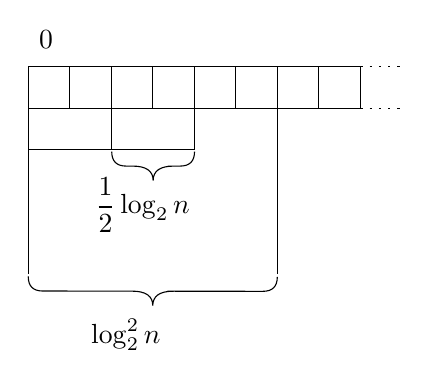
\begin{tikzpicture}[x=0.75pt,y=0.75pt,yscale=-1,xscale=1]
	\draw (150,231) .. controls (149.99,235.67) and (152.32,238) .. (156.99,238.01) -- (199.99,238.07) .. controls (206.66,238.08) and (209.99,240.41) .. (209.98,245.08) .. controls (209.99,240.41) and (213.32,238.09) .. (219.99,238.1)(216.99,238.09) -- (262.99,238.16) .. controls (267.66,238.17) and (269.99,235.84) .. (270,231.17);
	\draw (150,150) -- (150,230);
	\draw (270,150) -- (270,230);
	\draw (150,130) -- (170,130) -- (170,150) -- (150,150) -- cycle;
	\draw (170,130) -- (190,130) -- (190,150) -- (170,150) -- cycle;
	\draw (190,130) -- (210,130) -- (210,150) -- (190,150) -- cycle;
	\draw (210,130) -- (230,130) -- (230,150) -- (210,150) -- cycle;
	\draw (230,130) -- (250,130) -- (250,150) -- (230,150) -- cycle;
	\draw (250,130) -- (270,130) -- (270,150) -- (250,150) -- cycle;
	\draw (270,130) -- (290,130) -- (290,150) -- (270,150) -- cycle;
	\draw (290,130) -- (310,130) -- (310,150) -- (290,150) -- cycle;
	\draw (150,150) -- (190,150) -- (190,170) -- (150,170) -- cycle;
	\draw (190,150) -- (230,150) -- (230,170) -- (190,170) -- cycle;
	\draw (190.22,170.82) .. controls (190.22,175.49) and (192.55,177.82) .. (197.22,177.82) -- (200.17,177.82) .. controls (206.84,177.82) and (210.17,180.15) .. (210.17,184.82) .. controls (210.17,180.15) and (213.5,177.82) .. (220.17,177.82)(217.17,177.82) -- (223.11,177.82) .. controls (227.78,177.82) and (230.11,175.49) .. (230.11,170.82);
	\draw [dash pattern={on 0.84pt off 2.51pt}]  (310,130) -- (330,130);
	\draw [dash pattern={on 0.84pt off 2.51pt}]  (310,150) -- (330,150);

	\draw (179,250) node [anchor=north west][inner sep=0.75pt] [align=left] {$\displaystyle \log_2^2 n$};
	\draw (181,182) node [anchor=north west][inner sep=0.75pt] [align=left] {$\displaystyle \frac{1}{2} \log_2 n$};
	\draw (154,111.4) node [anchor=north west][inner sep=0.75pt] {$0$};
\end{tikzpicture}

	\caption{Divisione di $b$ in superblocchi e blocchi.}
	\label{fig:jrank}
\end{figure}

Si costruiscono quindi due vettori, $S$ e $B$. Per ogni superblocco $i$, $S_i$ contiene il rango del primo elemento di $b$ nel superblocco $i$. Per ogni blocco $j$, $B_j$ contiene la differenza tra il rango del primo elemento del blocco $j$ e il rango del primo elemento del relativo superblocco. Il rango di un elemento $p$ appartenente al superblocco $i$ e al blocco $j$ è quindi uguale a $S_i+B_j$ più il numero di bit a $1$ dall'inizio del blocco $j$ al bit $p$, ossia il rango di $p$ all'interno del sottovettore che coincide con il blocco $j$.

\begin{table}
	\centering
	\begin{tabular}{|c|c|c|c|c|c|c|}
		\hline
		\multirow{2}{*}{$0000$} & $p$        & $0$ & $1$ & $2$ & $3$ & $4$ \\ \cline{2-7}
		                        & $\rank(p)$ & $0$ & $0$ & $0$ & $0$ & $0$ \\ \hline
		\multirow{2}{*}{$0001$} & $p$        & $0$ & $1$ & $2$ & $3$ & $4$ \\ \cline{2-7}
		                        & $\rank(p)$ & $0$ & $0$ & $0$ & $0$ & $1$ \\ \hline
		$\cdots$                &            &     &     &     &     &     \\ \hline
		\multirow{2}{*}{$1111$} & $p$        & $0$ & $1$ & $2$ & $3$ & $4$ \\ \cline{2-7}
		                        & $\rank(p)$ & $0$ & $1$ & $2$ & $3$ & $4$ \\ \hline
	\end{tabular}
	\caption{Rango di ogni possibile blocco di lunghezza $4$.}
	\label{table:example_rank_block4}
\end{table}

I ranghi delle posizioni in un blocco sono salvati in un'apposita tabella, per evitare di doverli calcolare ogni volta. È quindi necessaria una tabella (simile a quanto mostrato in \cref{table:example_rank_block4}) che contiene il rango di ogni posizione, per ogni possibile tipo di blocco. I tipi di blocco possibili sono, in numero:
\begin{equation*}
	2^{\frac{1}{2}\log_2 n} = \left(2^{\log_2 n}\right)^{\frac{1}{2}} = \sqrt{n}
\end{equation*}

Il costo in bit di ogni tabella è
\begin{equation*}
	\underbrace{\frac{1}{2}\log_2 n}_\text{numero di elementi}\cdot \underbrace{\log_2\left(\frac{1}{2}\log_2 n\right)}_\text{costo dei valori di rango}
\end{equation*}
per un totale, per tutte le tabelle, di
\begin{equation*}
	\sqrt n\cdot\frac{1}{2}\log_2 n\cdot \log_2\left(\frac{1}{2}\log_2 n\right)
	\leq \sqrt n\cdot \frac{1}{2}\log_2 n\cdot \log_2(\log_2 n) = o(n) \text{ bit.}
\end{equation*}

Lo spazio occupato dal vettore $S$ è
\begin{equation*}
	\underbrace{\frac{n}{\log_2^2 n}}_\text{numero di superblocchi}\cdot\underbrace{\log_2 n}_\text{costo del singolo valore} = \frac{n}{\log_2 n} = o(n) \text{ bit}
\end{equation*}
Mentre quello occupato dal vettore $B$ è
\begin{equation*}
	\underbrace{\frac{n}{\frac{1}{2}\log_2 n}}_\text{numero di blocchi} \cdot\log_2(\log_2^2 n) =
	\frac{2n}{\log_2 n} 2 \log_2(\log_2 n) = o(n) \text{ bit}
\end{equation*}

% TODO migliorare figura (blocchi di 2 non sono molto rappresentativi)
\begin{figure}
	\centering
	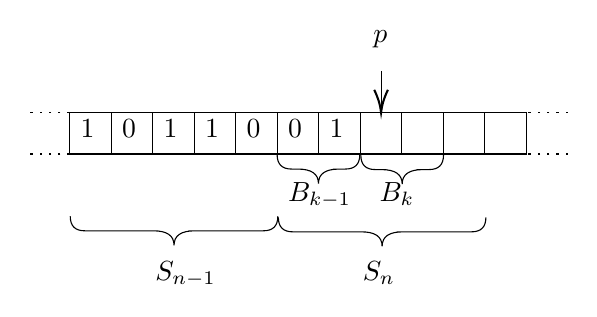
\begin{tikzpicture}[x=0.75pt,y=0.75pt,yscale=-1,xscale=1]
	\draw (100,100) -- (320,100) -- (320,120) -- (100,120) -- cycle;
	\draw (120,100) -- (120,120);
	\draw (140,100) -- (140,120);
	\draw (160,100) -- (160,120);
	\draw (180,100) -- (180,120);
	\draw (200,100) -- (200,120);
	\draw (220,100) -- (220,120);
	\draw (240,100) -- (240,120);
	\draw (260,100) -- (260,120);
	\draw (280,100) -- (280,120);
	\draw (300,100) -- (300,120);
	\draw (250,80) -- (250,98);
	\draw [shift={(250,100)}, rotate = 270] [color={rgb, 255:red, 0; green, 0; blue, 0 }  ][line width=0.75]    (10.93,-3.29) .. controls (6.95,-1.4) and (3.31,-0.3) .. (0,0) .. controls (3.31,0.3) and (6.95,1.4) .. (10.93,3.29);
	\draw (100.25,150) .. controls (100.25,154.67) and (102.58,157) .. (107.25,157) -- (140.25,157) .. controls (146.92,157) and (150.25,159.33) .. (150.25,164) .. controls (150.25,159.33) and (153.58,157) .. (160.25,157)(157.25,157) -- (193.25,157) .. controls (197.92,157) and (200.25,154.67) .. (200.25,150);
	\draw (200.5,150.5) .. controls (200.5,155.17) and (202.83,157.5) .. (207.5,157.5) -- (240.5,157.5) .. controls (247.17,157.5) and (250.5,159.83) .. (250.5,164.5) .. controls (250.5,159.83) and (253.83,157.5) .. (260.5,157.5)(257.5,157.5) -- (293.5,157.5) .. controls (298.17,157.5) and (300.5,155.17) .. (300.5,150.5);
	\draw [dash pattern={on 0.84pt off 2.51pt}] (100,100) -- (80,100);
	\draw [dash pattern={on 0.84pt off 2.51pt}] (100,120) -- (80,120);
	\draw [dash pattern={on 0.84pt off 2.51pt}] (340,120) -- (320,120);
	\draw [dash pattern={on 0.84pt off 2.51pt}] (340,100) -- (320,100);
	\draw (240.25,120.5) .. controls (240.25,125.17) and (242.58,127.5) .. (247.25,127.5) -- (250.17,127.5) .. controls (256.84,127.5) and (260.17,129.83) .. (260.17,134.5) .. controls (260.17,129.83) and (263.5,127.5) .. (270.17,127.5)(267.17,127.5) -- (273.08,127.5) .. controls (277.75,127.5) and (280.08,125.17) .. (280.08,120.5);
	\draw (199.92,120.25) .. controls (199.92,124.92) and (202.25,127.25) .. (206.92,127.25) -- (209.83,127.25) .. controls (216.5,127.25) and (219.83,129.58) .. (219.83,134.25) .. controls (219.83,129.58) and (223.16,127.25) .. (229.83,127.25)(226.83,127.25) -- (232.75,127.25) .. controls (237.42,127.25) and (239.75,124.92) .. (239.75,120.25);
	\draw (245,59.4) node [anchor=north west][inner sep=0.75pt] {$p$};
	\draw (104,102.4) node [anchor=north west][inner sep=0.75pt] {$1$};
	\draw (124,102.4) node [anchor=north west][inner sep=0.75pt] {$0$};
	\draw (144,102.4) node [anchor=north west][inner sep=0.75pt] {$1$};
	\draw (224,102.4) node [anchor=north west][inner sep=0.75pt] {$1$};
	\draw (164,102.4) node [anchor=north west][inner sep=0.75pt] {$1$};
	\draw (204,102.4) node [anchor=north west][inner sep=0.75pt] {$0$};
	\draw (240,170.4) node [anchor=north west][inner sep=0.75pt] {$S_{n}$};
	\draw (140,170.4) node [anchor=north west][inner sep=0.75pt] {$S_{n-1}$};
	\draw (248,132.4) node [anchor=north west][inner sep=0.75pt] {$B_{k}$};
	\draw (204,132.4) node [anchor=north west][inner sep=0.75pt] {$B_{k-1}$};
	\draw (184,102.4) node [anchor=north west][inner sep=0.75pt] {$0$};
\end{tikzpicture}

	\caption{Calcolo di $\rank(p)$.}
	\label{fig:example_rank_p}
\end{figure}

Un'implementazione della struttura succinta di Jacobson per il rango impiega un tempo costante per calcolare il rango di una posizione $p$, dovendo effettuare un accesso ai vettori $S$ e $B$ e uno alla tabella dei tipi di blocco. In effetti l'identificazione del tipo di blocco, stando al criterio di costo della macchina di Turing, è logaritmica in $n$, dovendo scansionare linearmente il blocco che contiene la posizione interessata. Tuttavia, adottando un criterio di costo simile alle macchine reali, questa scansione avviene in tempo costante, poiché un blocco è solitamente contenuto in una o due parole di memoria, recuperate in tempo costante.


\subsection{Struttura di Clarke per la selezione}
La struttura di Clarke per la selezione è succinta teoricamente, ma in pratica
è raramente utilizzata come descritta perché la sua implementazione è molto
complessa.
L'obiettivo è, dato un vettore $\mathbf{b}$ di valori binari fissato, calcolare
la funzione di selezione
$$
	\mathbf{select_b}(k) = \text{ posizione del } k-\text{esimo } 1
$$
La struttura di Clarke utilizza dei \textit{livelli}, simili a quelli utilizzati
dalla struttura di Jacobson.

\subsubsection{Primo livello}
Il primo livello della struttura di Clarke è un insieme
di valori che rappresentano le posizioni degli $1$ di ordinalità multipla di
$\log_2(n) \cdot \log_2(\log_2(n))$, ossia
$$
	P_i =  \mathbf{select_b}(i \cdot \log_2(n) \cdot \log_2(\log_2(n)))
$$
ossia la posizione del $(i \cdot \log_2(n) \cdot \log_2(\log_2(n)))$-esimo $1$.

\paragraph{Memoria}
La grandezza di questa famiglia, ossia il numero di $P_i$, dipende dal
numero di $i$ che ci sono in $\mathbf{b}$, ma nel caso peggiore, il vettore
è composto unicamente da $1$ e vi saranno $\frac{n}{\log_2(n) \cdot \log_2(\log_2(n))}$ membri.
Ad ognuno di essi va associato un elemento, il quale richiede $\log_2(n)$ bit;
in totale, questo livello occupa
$$
	\frac{n}{\log_2(n) \cdot \log_2(\log_2(n))} \cdot \log_2(n) = o(n) \text{ bit}
$$

\subsubsection{Secondo livello}
Per le posizioni che non sono multiple di $\log_2(n) \cdot \log_2(\log_2(n))$ si utilizza
un secondo livello, che è costruito differentemente in base ad un indice calcolato
per ogni $P_i$:

$$
	\forall i ~ r_i = P_{i + 1} - P_i
$$
che rappresenta la distanza fra l'$(i \cdot \log_2(n) \cdot \log_2(\log_2(n)))$-esimo $1$
e il $((i+1) \cdot \log_2(n) \cdot \log_2(\log_2(n)))$-esimo. Questo
valore, $r_i$, sarà esattamente uguale a $\log_2(n) \cdot \log_2(\log_2(n))$ se e solo se
tra $P_{i}$ e $P_{i+1}$ ci sono unicamente $1$, e sarà maggiore se invece le
due posizioni sono più lontane.
% @TODO: serve un esempio, non si capisce bene. 
I due casi che si considerano dipendono dal valore di $r_i$.

\paragraph{Caso sparso}
Se $r_i \geq (\log_2(n) \cdot \log_2(\log_2(n)))^2$, significa che in $\mathbf{b}$ ci
sono molti $0$ tra gli $1$ contenuti nelle posizioni tra $P_{i}$ e $P_{i+1}$; in questo caso
definiamo $S_i$ come la lista esplicita delle posizioni di tutti gli $1$
in $\mathbf{b}$ tra le due posizioni rappresentate come differenza tra $P_i$.

In questo caso, gli $S_i$ costruiti sono esattamente $\log_2(n)\cdot \log_2(\log_2(n))$,
in quanto stiamo contando gli $1$ in $\mathbf{b}$ tra il $(i \cdot \log_2(n) \cdot \log_2(\log_2(n))$-esimo
$1$ e il $((i+1) \cdot \log_2(n) \cdot \log_2(\log_2(n))$-esimo $1$, e ad ognuno
di essi si associa un numero che in grandezza è minore o uguale a
$\log_2(r_i)$, concludendo che per memorizzare un $S_i$ sono necessari
\begin{align*}
	\log_2(n)\cdot \log_2(\log_2(n)) \cdot \log_2(r_i) & = \frac{(\log_2(n)\cdot \log_2(\log_2(n)))^2}{\log_2(n)\cdot \log_2(\log_2(n))} \cdot \log_2(r_i) \\
	                                                   & \leq \frac{r_i}{\log_2(n)\cdot \log_2(\log_2(n))} \cdot \log_2(r_i)                               \\
	                                                   & \leq \frac{r_i}{\log_2(n)\cdot \log_2(\log_2(n))} \cdot \log_2(n)                                 \\
	                                                   & \leq \frac{r_i}{\log_2(\log_2(n))}                                                                \\
	                                                   & \leq \frac{n}{\log_2(\log_2(n))}   = o(n) \text{ bit}
\end{align*}

\paragraph{Caso denso}
Se $r_i \le (\log_2(n) \cdot \log_2(\log_2(n)))^2$, si memorizzano gli $1$
multipli di $\log_2(r_i)\log_2(\log_2(n))$, ossia partendo dalla posizione $P_i$ si salvano le
posizioni degli $j \cdot \log_2(r_i)\log_2(\log_2(n))$-esimi $1$ come differenze da $P_i$, ossia
$$
	S^i_j = \mathbf{select_b}(j \cdot \log_2(r_i)\log_2(\log_2(n))) - P_i
$$

In questo caso, gli $1$ memorizzati sono $\frac{\log_2(n)\cdot \log_2(\log_2(n))}{\log_2(r_i)\cdot \log_2(\log_2(n))}$.
Ad ognuno di questi si associa un valore in grandezza $\log_2(r_i)$, quindi lo spazio utilizzato
per memorizzare tutti i valori $S^i_j$ sono
$$
	\frac{\log_2(n)\cdot \log_2(\log_2(n))}{\log_2(r_i)\cdot \log_2(\log_2(n))} \log_2(r_i) =
	\frac{\log_2(n)\cdot \log_2(\log_2(n))}{\log_2(\log_2(n))} \leq \frac{r_i}{\log_2(\log_2(n))}
	\leq \frac{n}{\log_2(\log_2(n))} = o(n) \text{ bit}
$$


\subsubsection{Terzo livello}
Se nel secondo livello ci si trova nel caso denso, si utilizza un terzo livello.
Questo livello viene utilizzato esclusivamente per gli $1$ le cui posizioni non sono state
salvate nel secondo livello nel caso denso; pertanto, l'assunto è che
$$
	r_i < (\log_2(n) \log_2(\log_2(n)))^2
$$
Per ognuna di queste posizioni calcoliamo la differenza tra $S^i_j$:
$$
	\forall j ~~ \bar{r}^i_j = S^i_{j+1} - S^i_j
$$
Come nel caso precedente, abbiamo due possibilità in base al valore di $\bar{r}^i_j$, il quale
gode comunque della proprietà
$$
	\forall i, j ~~  \bar{r}^i_j \geq \log_2(r_i) \log_2(\log_2(n))
$$
\paragraph{Caso sparso}
Nel caso in cui $\bar{r}^i_j \geq \log_2(\bar{r}^i_j) \log_2(r_i) \log_2(\log_2(n))^2$,
si memorizzano esplicitamente tutte le posizioni degli $1$ tra $S^i_j$ e $S^i_{j+1}$
con dei valori $T^i_{j,k}$ come differenze tra $S^i_j$. In questo caso,
il consumo di memoria è
$$
	(\log_2(r_i)\cdot \log_2(\log_2(n)) \cdot \log_2(\bar{r}^i_j) \leq
	\frac{\log_2(r_i) \cdot \log_2(\log_2(n))^2 \log_2(\bar{r}^i_j)}{\log_2(\log_2(n))}
	\leq \frac{\bar{r}^i_j}{\log_2(\log_2(n))} = o(n) \text{ bit}
$$
\paragraph{Caso denso}
Nel caso in cui $\bar{r}^i_j \le \log_2(\bar{r}^i_j) \log_2(r_i) \log_2(\log_2(n))^2$,
significa che ci sono pochi $0$ tra $S^i_j$ e $S^i_{j+1}$ e
si utilizza il four-russians trick. Inizialmente osserviamo quanto segue.
\begin{oss}
	\begin{align*}
		\log_2(\bar{r}^i_j) \leq \log_2(r_i) & \leq \log_2(\log_2(n)\cdot \log_2(\log_2(n)))^2     \\
		                                     & = 2 \log_2(\log_2(n)) + 2 \log_2(\log_2(\log_2(n))) \\
		                                     & \leq 4 \log_2(\log_2(n))
	\end{align*}
\end{oss}
\begin{oss}
	$$
		\bar{r}^i_j < \log_2(\bar{r}^i_j) \cdot \log_2(r_i) \cdot (\log_2(\log_2(n))^2
		\leq 16(\log_2\log_2(n))^4
	$$
\end{oss}
Lo spazio necessario per utilizzare il four-russians trick è quanto segue.
Servono $2^{\bar{r}^i_j}$ enumerazioni di `sottovettori',
ossia la dimensione tra $S^i_j$ e $S^i_{j+1}$,
che è la parte che va memorizzata esplicitamente; per ognuna di queste
enumerazioni è necessario salvare la posizione di $\bar{r}^i_j$ $1$ utilizzando
memoria al massimo $\log_2(\bar{r}^i_j)$:
\begin{align*}
	2^{\bar{r}^i_j} \cdot \bar{r}^i_j \cdot \log_2(\bar{r}^i_j) & \leq
	2^{16(\log_2\log_2(n))^4} \cdot 16(\log_2\log_2(n))^4 \cdot \log_2(16(\log_2\log_2(n))^4)                                  \\
	                                                            & = 16(\log_2\log_2(n))^8 \log_2(16(\log_2\log_2(n))^4) = o(n)
\end{align*}


\subsubsection{Complessità totale in spazio}
In totale, per memorizzare $\mathbf{b}$ e i possibili tre livelli di struttura,
sono necessari $o(n)$ bit per il primo livello e, in base a come è fatto il secondo livello
$$
	\sum^{\frac{n}{\log_2(n)\cdot \log_2(\log_2(n))}} \frac{P_{i+1} - P_i}{\log_2(\log_2(n)}
	= \frac{P_n - P_0}{\log_2(\log_2(n))}
	\leq \frac{n}{\log_2(\log_2(n))} = o(n) \text{ bit}
$$
più $o(n)$ bit per il terzo livello. Quindi, la struttura di Clarke occupa
spazio $n + o(n)$ e ha tempo di accesso costante, pertanto è
una struttura \textbf{succinta}.

\begin{figure}
	\centering
	\tikzset{every picture/.style={line width=0.75pt}} %set default line width to 0.75pt        

	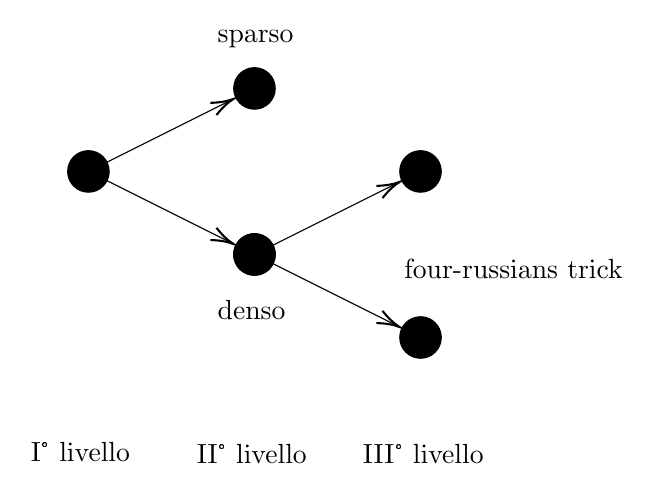
\begin{tikzpicture}[x=0.75pt,y=0.75pt,yscale=-1,xscale=1]
		%uncomment if require: \path (0,300); %set diagram left start at 0, and has height of 300

		%Shape: Circle [id:dp9914836432536758] 
		\draw  [fill={rgb, 255:red, 0; green, 0; blue, 0 }  ,fill opacity=1 ] (70,101) .. controls (70,95.48) and (74.48,91) .. (80,91) .. controls (85.52,91) and (90,95.48) .. (90,101) .. controls (90,106.52) and (85.52,111) .. (80,111) .. controls (74.48,111) and (70,106.52) .. (70,101) -- cycle ;
		%Shape: Circle [id:dp09703813871749656] 
		\draw  [fill={rgb, 255:red, 0; green, 0; blue, 0 }  ,fill opacity=1 ] (150,61) .. controls (150,55.48) and (154.48,51) .. (160,51) .. controls (165.52,51) and (170,55.48) .. (170,61) .. controls (170,66.52) and (165.52,71) .. (160,71) .. controls (154.48,71) and (150,66.52) .. (150,61) -- cycle ;
		%Straight Lines [id:da8346853138498954] 
		\draw    (80,101) -- (148.21,66.89) ;
		\draw [shift={(150,66)}, rotate = 153.43] [color={rgb, 255:red, 0; green, 0; blue, 0 }  ][line width=0.75]    (10.93,-3.29) .. controls (6.95,-1.4) and (3.31,-0.3) .. (0,0) .. controls (3.31,0.3) and (6.95,1.4) .. (10.93,3.29)   ;
		%Shape: Circle [id:dp4565729376211175] 
		\draw  [fill={rgb, 255:red, 0; green, 0; blue, 0 }  ,fill opacity=1 ] (150,141) .. controls (150,146.52) and (154.48,151) .. (160,151) .. controls (165.52,151) and (170,146.52) .. (170,141) .. controls (170,135.48) and (165.52,131) .. (160,131) .. controls (154.48,131) and (150,135.48) .. (150,141) -- cycle ;
		%Straight Lines [id:da8127484960209145] 
		\draw    (80,101) -- (148.21,135.11) ;
		\draw [shift={(150,136)}, rotate = 206.57] [color={rgb, 255:red, 0; green, 0; blue, 0 }  ][line width=0.75]    (10.93,-3.29) .. controls (6.95,-1.4) and (3.31,-0.3) .. (0,0) .. controls (3.31,0.3) and (6.95,1.4) .. (10.93,3.29)   ;
		%Shape: Circle [id:dp546530222511162] 
		\draw  [fill={rgb, 255:red, 0; green, 0; blue, 0 }  ,fill opacity=1 ] (150,141) .. controls (150,135.48) and (154.48,131) .. (160,131) .. controls (165.52,131) and (170,135.48) .. (170,141) .. controls (170,146.52) and (165.52,151) .. (160,151) .. controls (154.48,151) and (150,146.52) .. (150,141) -- cycle ;
		%Shape: Circle [id:dp1691093585413369] 
		\draw  [fill={rgb, 255:red, 0; green, 0; blue, 0 }  ,fill opacity=1 ] (230,101) .. controls (230,95.48) and (234.48,91) .. (240,91) .. controls (245.52,91) and (250,95.48) .. (250,101) .. controls (250,106.52) and (245.52,111) .. (240,111) .. controls (234.48,111) and (230,106.52) .. (230,101) -- cycle ;
		%Straight Lines [id:da17118221437478087] 
		\draw    (160,141) -- (228.21,106.89) ;
		\draw [shift={(230,106)}, rotate = 153.43] [color={rgb, 255:red, 0; green, 0; blue, 0 }  ][line width=0.75]    (10.93,-3.29) .. controls (6.95,-1.4) and (3.31,-0.3) .. (0,0) .. controls (3.31,0.3) and (6.95,1.4) .. (10.93,3.29)   ;
		%Shape: Circle [id:dp8870903616648642] 
		\draw  [fill={rgb, 255:red, 0; green, 0; blue, 0 }  ,fill opacity=1 ] (230,181) .. controls (230,186.52) and (234.48,191) .. (240,191) .. controls (245.52,191) and (250,186.52) .. (250,181) .. controls (250,175.48) and (245.52,171) .. (240,171) .. controls (234.48,171) and (230,175.48) .. (230,181) -- cycle ;
		%Straight Lines [id:da2110125336208042] 
		\draw    (160,141) -- (228.21,175.11) ;
		\draw [shift={(230,176)}, rotate = 206.57] [color={rgb, 255:red, 0; green, 0; blue, 0 }  ][line width=0.75]    (10.93,-3.29) .. controls (6.95,-1.4) and (3.31,-0.3) .. (0,0) .. controls (3.31,0.3) and (6.95,1.4) .. (10.93,3.29)   ;

		% Text Node
		\draw (51,230) node [anchor=north west][inner sep=0.75pt]   [align=left] {I° livello};
		% Text Node
		\draw (131,231) node [anchor=north west][inner sep=0.75pt]   [align=left] {II° livello};
		% Text Node
		\draw (211,231) node [anchor=north west][inner sep=0.75pt]   [align=left] {III° livello};
		% Text Node
		\draw (141,162) node [anchor=north west][inner sep=0.75pt]   [align=left] {denso};
		% Text Node
		\draw (141,32) node [anchor=north west][inner sep=0.75pt]   [align=left] {sparso};
		% Text Node
		\draw (231,142) node [anchor=north west][inner sep=0.75pt]   [align=left] {four-russians trick};
	\end{tikzpicture}
	\caption{Struttura di Clarke per la selezione.}
\end{figure}



\section{Alberi binari}
Un albero è un grafo non orientato, connesso e aciclico.
Un albero con radice è un albero in cui si elegge un vertice radice. I vertici adiacenti alla radice sono i suoi figli, che danno origine a sottoalberi. I vertici che danno origine a sottoalberi composti unicamente dalla radice sono detti foglie, o nodi esterni. I rimanenti nodi in un albero sono detti nodi interni.
Un albero binario è un albero radicato in cui ogni nodo interno ha due figli.
Equivalentemente si possono definire gli alberi binari induttivamente: un albero binario è una foglia $\emptyset$, oppure, se $L$ e $R$ sono alberi binari, è una coppia $(L,R)$ composta da una radice a cui sono connessi i sottoalberi $L$ e $R$.

% TODO: migliorare figura del passo induttivo: la radice dovrebbe essere adiacente alle radici dei sottoalberi
\begin{figure}
	\begin{subfigure}{0.45\textwidth}
	\begin{center}
		
\begin{tikzpicture}
			\node [circle,draw]{};
		\end{tikzpicture}
	\end{center}
	\caption{Foglia}
\end{subfigure}
\begin{subfigure}{0.45\textwidth}
	\begin{center}
		\begin{tikzpicture}[subtree/.style={isosceles triangle,draw,shape border rotate=90}]
			\node[circle,draw] {}
			child { node[subtree] {$T_1$} }
			child { node[subtree] {$T_2$} };
		\end{tikzpicture}
	\end{center}
	\caption{Radice con due sottoalberi}
\end{subfigure}

	\caption{Definizione induttiva di albero binario.}
	\label{fig:btree_inductive}
\end{figure}

Un albero può essere \emph{ancillare}, cioè organizzare dati contenuti nei nodi interni o nelle foglie (tipicamente esclusivamente una delle due opzioni). Le strutture costruite per alberi privi di dati possono tipicamente essere generalizzate al caso di alberi ancillari.

Dato un albero binario, chiameremo $E$ l'insieme dei nodi esterni (foglie), $I$ l'insieme dei nodi interni e $n:=\card{I}$.
Definiamo inoltre le funzioni $\trext$ e $\trint$, definite rispettivamente come il numero di foglie e nodi interni di un dato albero binario.

\begin{theorem}\label{thm:btree_leaves}
	In un albero binario, il numero di foglie è uguale al numero di nodi interni più uno:
	\begin{equation*}
		\card{I}=\card{E}+1
	\end{equation*}
\end{theorem}
\begin{proof}
	Effettuando induzione strutturale sulla definizione di albero binario:
	\begin{itemize}
		\item $\trext(\emptyset)=1$, $\trint(\emptyset)=0$.
		\item siano $L, R$ due alberi binari. Vale
		      \begin{equation*}
			      \trext((L,R)) = \trext(L) + \trext(R) = \trint(L) + 1 + \trint(R) + 1 = \trint((L, R))  + 1
		      \end{equation*}
	\end{itemize}
\end{proof}

\begin{corollario}
	Ogni albero con $n$ nodi interni ha in totale $2n+1$ nodi.
\end{corollario}

\begin{theorem}\label{thm:catalano}
	Il numero di alberi binari con $n$ nodi interni è $C_n$, dove $C_n$ è l'$n$-esimo numero di Catalano:
	\begin{equation*}
		C_n := \frac{1}{n+1}\binom{2n}{n}
	\end{equation*}
\end{theorem}
\begin{corollario}
	\begin{equation*}
		\forall n \quad\log_2(C_n)=2n+O(\log_2(n))
	\end{equation*}
\end{corollario}
\begin{proof}
	Ricordando l'approssimazione di Stirling per il fattoriale:
	\begin{equation*}
		x! \sim \sqrt{2\pi x} \left(\frac{x}{e}\right)^x
	\end{equation*}
	si ha che
	\begin{align*}
		C_n = \frac{1}{n+1}\binom{2n}{n} & = \frac{1}{n+1}\cdot\frac{(2n)!}{n!(2n-n)!}                                                             \\
		                                 & = \frac{(2n)!}{(n+1)(n!)^2}                                                                             \\
		                                 & \sim \frac{\sqrt{4\pi n}\left(\frac{2n}{e}\right)^{2n}}{(n+1)\cdot 2\pi n\left(\frac{n}{e}\right)^{2n}} \\
		                                 & = \frac{1}{n+1}\cdot \frac{1}{\sqrt{\pi n}}\cdot 2^{2n}                                                 \\
		                                 & \approx \frac{4^n}{\sqrt{\pi n^3}}
	\end{align*}
	Da cui
	% TODO: spiegare
	\begin{equation*}
		\log_2 C_n = 2n-O(\log n) \text.
	\end{equation*}
\end{proof}
\begin{corollario}\label{corol:bitree:itlb}
	L'information theoretical lower bound in bit per gli alberi binari è
	\begin{equation*}
		Z_n = 2n-O(\log_2(n)) \text.
	\end{equation*}
\end{corollario}


\subsection{Una struttura succinta per alberi binari}
Per costruire una struttura succinta per gli alberi binari, definiamo tre operazioni fondamentali in cui possono consistere le query alla struttura dati: le operazioni $\trleft$ e $\trright$, che restituiscono rispettivamente il figlio sinistro e destro di un dato nodo, e l'operazione $\trparent$, che restituisce il genitore di un dato nodo.

Per rappresentare un albero binario con $n$ nodi interni, numeriamo i nodi da $0$ a $2n$ seguendo una visita in ampiezza, come rappresentato in \cref{fig:btree_rappr_num}.
Costruiamo quindi un vettore $v$ (\cref{fig:btree_rappr_vec}), di lunghezza $2n+1$ e tale che
\begin{equation*}
	\forall i\in\set{0,\dots,2n},\qquad v_i = \begin{cases}
		1 & \text{se il nodo $i$ appartiene a $I$} \\
		0 & \text{altrimenti}
	\end{cases}
\end{equation*}

\begin{figure}
	\centering
	\begin{subfigure}[t]{0.45\textwidth}
	\centering
	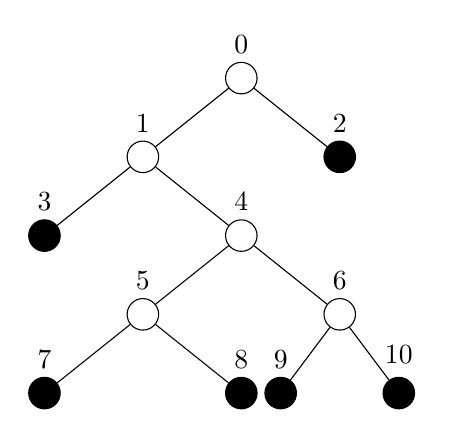
\begin{tikzpicture}[
			every node/.style={circle, draw, minimum size=4mm, inner sep=0.5mm},
			level distance=10mm,
			level 1/.style={sibling distance=25mm},
			level 2/.style={sibling distance=25mm}]
		\node [label=above:{0}]{}
		child {
		node [label=above:{1}] {}
		child {node[fill, label=above:{3}]{}}
		child {
		node[label=above:{4}]{}
		child {
		node [label=above:{5}]{}
		child {node[fill,label=above:{7}]{}}
		child {node[fill,label=above:{8}]{}}
		}
		child {
		node[label=above:{6}]  {}
		[level distance=10mm ,sibling distance=15mm]
		child {node[fill,label=above:{9}] {}}
		child {node[fill,label=above:{10}] {}}
		}
		}
		}
		child {node [fill, label=above:{2}]{}};
	\end{tikzpicture}

	\caption{Albero binario numerato.}
	\label{fig:btree_rappr_num}
\end{subfigure}
\begin{subfigure}[t]{0.45\textwidth}
	\centering
	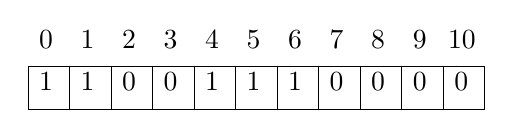
\begin{tikzpicture}[x=0.75pt,y=0.75pt,yscale=-1,xscale=1]
		\draw   (160,120) -- (180,120) -- (180,140.67) -- (160,140.67) -- cycle;
		\draw   (180,120) -- (200,120) -- (200,140.67) -- (180,140.67) -- cycle;
		\draw   (200,120) -- (220,120) -- (220,140.67) -- (200,140.67) -- cycle;
		\draw   (220,120) -- (240,120) -- (240,140.67) -- (220,140.67) -- cycle;
		\draw   (240,120) -- (260,120) -- (260,140.67) -- (240,140.67) -- cycle;
		\draw   (260,120) -- (280,120) -- (280,140.67) -- (260,140.67) -- cycle;
		\draw   (280,120) -- (300,120) -- (300,140.67) -- (280,140.67) -- cycle;
		\draw   (300,120) -- (320,120) -- (320,140.67) -- (300,140.67) -- cycle;
		\draw   (320,120) -- (340,120) -- (340,140.67) -- (320,140.67) -- cycle;
		\draw   (340,120) -- (360,120) -- (360,140.67) -- (340,140.67) -- cycle;
		\draw   (360,120) -- (380,120) -- (380,140.67) -- (360,140.67) -- cycle;
		\draw (164,101.4) node [anchor=north west][inner sep=0.75pt]    {$0$};
		\draw (184,101.4) node [anchor=north west][inner sep=0.75pt]    {$1$};
		\draw (204,101.4) node [anchor=north west][inner sep=0.75pt]    {$2$};
		\draw (224,101.4) node [anchor=north west][inner sep=0.75pt]    {$3$};
		\draw (244,101.4) node [anchor=north west][inner sep=0.75pt]    {$4$};
		\draw (264,101.4) node [anchor=north west][inner sep=0.75pt]    {$5$};
		\draw (284,101.4) node [anchor=north west][inner sep=0.75pt]    {$6$};
		\draw (304,101.4) node [anchor=north west][inner sep=0.75pt]    {$7$};
		\draw (324,101.4) node [anchor=north west][inner sep=0.75pt]    {$8$};
		\draw (344,101.46) node [anchor=north west][inner sep=0.75pt]    {$9$};
		\draw (361,101.4) node [anchor=north west][inner sep=0.75pt]    {$10$};
		\draw (164,121.4) node [anchor=north west][inner sep=0.75pt]    {$1$};
		\draw (184,121.4) node [anchor=north west][inner sep=0.75pt]    {$1$};
		\draw (204,121.4) node [anchor=north west][inner sep=0.75pt]    {$0$};
		\draw (224,121.4) node [anchor=north west][inner sep=0.75pt]    {$0$};
		\draw (244,121.4) node [anchor=north west][inner sep=0.75pt]    {$1$};
		\draw (264,121.4) node [anchor=north west][inner sep=0.75pt]    {$1$};
		\draw (284,121.4) node [anchor=north west][inner sep=0.75pt]    {$1$};
		\draw (304,121.4) node [anchor=north west][inner sep=0.75pt]    {$0$};
		\draw (324,121.4) node [anchor=north west][inner sep=0.75pt]    {$0$};
		\draw (344,121.46) node [anchor=north west][inner sep=0.75pt]    {$0$};
		\draw (364,121.4) node [anchor=north west][inner sep=0.75pt]    {$0$};
	\end{tikzpicture}
	\caption{Vettore associato all'albero.}
	\label{fig:btree_rappr_vec}
\end{subfigure}

	\caption{Un albero binario e il suo vettore associato.}
\end{figure}

Studiamo ora come produrre i risultati delle query di $\trleft$, $\trright$, e $\trparent$ a partire dal vettore $v$. Si consideri, all'interno di un albero $T$, una terna di nodi $p,q,q+1$, dove $p$ è il genitore e $q$ e $q+1$ i figli. Sia $T'$ il sottoalbero radicato nella stessa radice di $T$ contenente tutti i nodi di numero minore di $q$, come rappresentato in \cref{fig:btree_rappr_step}. Si tenga presente che alcuni nodi interni nell'albero $T$, in particolare quelli che seguono $p$, diventano foglie in $T'$.

Il numero di nodi interni minori di $p$, ossia il numero di nodi interni in $T'$, è uguale al rango di $p$ in $v$. Applicando il \cref{thm:btree_leaves}, calcoliamo che il numero complessivo di nodi minori di $q$, cioè il numero di nodi dell'albero $T'$, è
\begin{equation}\label{eq:btree:left_child}
	\trleft(p) = q = \trint(T')+\trext(T') = 2\cdot\trint(T')+1 = 2\cdot\rank(p)+1 \text.
\end{equation}
Mentre per il figlio destro vale, ovviamente
\begin{equation}\label{eq:btree:right_child}
	\trright(p) = q+1 = 2\cdot\rank(p)+1 \text.
\end{equation}

\begin{figure}
	\centering
	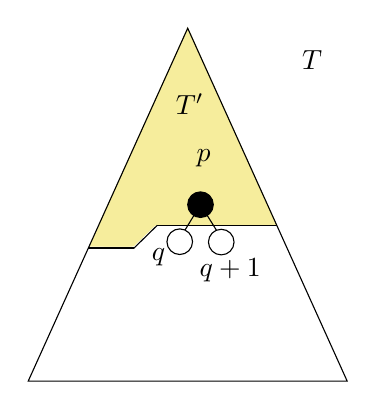
\begin{tikzpicture}[x=0.75pt,y=0.75pt,yscale=-1,xscale=1]
	\draw  [color={rgb, 255:red, 246; green, 237; blue, 156 }  ,draw opacity=1 ][fill={rgb, 255:red, 246; green, 237; blue, 156 }  ,fill opacity=1 ] (312.92,126.04) -- (317.75,115.9) -- (328.33,115.9) -- (333.17,126.04) -- cycle;
	\draw  [color={rgb, 255:red, 246; green, 237; blue, 156 }  ,draw opacity=1 ][fill={rgb, 255:red, 246; green, 237; blue, 156 }  ,fill opacity=1 ] (346,114.3) -- (334.2,125.7) -- (334.2,114.3) -- cycle;
	\draw  [color={rgb, 255:red, 246; green, 237; blue, 156 }  ,draw opacity=1 ][fill={rgb, 255:red, 246; green, 237; blue, 156 }  ,fill opacity=1 ] (360.11,21.08) -- (402.87,115.9) -- (317.34,115.9) -- cycle;
	\draw  [fill={rgb, 255:red, 0; green, 0; blue, 0 }  ,fill opacity=1 ] (360.11,106.08) .. controls (360.11,102.68) and (362.87,99.92) .. (366.28,99.92) .. controls (369.68,99.92) and (372.44,102.68) .. (372.44,106.08) .. controls (372.44,109.49) and (369.68,112.25) .. (366.28,112.25) .. controls (362.87,112.25) and (360.11,109.49) .. (360.11,106.08) -- cycle;
	\draw    (366.28,106.08) -- (356.04,122.86);
	\draw    (366.28,106.08) -- (376.09,121.82);
	\draw   (360.11,21.08) -- (436.94,191.08) -- (283.28,191.08) -- cycle;
	\draw    (312.18,126.95) -- (334.47,126.95);
	\draw    (345.08,116.14) -- (402.93,116.14);
	\draw    (345.49,115.99) -- (333.99,127.24);
	\draw  [fill={rgb, 255:red, 255; green, 255; blue, 255 }  ,fill opacity=1 ] (350.11,123.93) .. controls (350.11,120.53) and (352.87,117.76) .. (356.28,117.76) .. controls (359.68,117.76) and (362.44,120.53) .. (362.44,123.93) .. controls (362.44,127.34) and (359.68,130.1) .. (356.28,130.1) .. controls (352.87,130.1) and (350.11,127.34) .. (350.11,123.93) -- cycle;
	\draw  [fill={rgb, 255:red, 255; green, 255; blue, 255 }  ,fill opacity=1 ] (370.11,124.11) .. controls (370.11,120.71) and (372.87,117.95) .. (376.28,117.95) .. controls (379.68,117.95) and (382.44,120.71) .. (382.44,124.11) .. controls (382.44,127.52) and (379.68,130.28) .. (376.28,130.28) .. controls (372.87,130.28) and (370.11,127.52) .. (370.11,124.11) -- cycle;
	\draw  [color={rgb, 255:red, 246; green, 237; blue, 156 }  ,draw opacity=1 ][fill={rgb, 255:red, 246; green, 237; blue, 156 }  ,fill opacity=1 ] (320.12,125.88) -- (333.92,109.62) -- (333.95,125.85) -- cycle;
	\draw (341.53,125.76) node [anchor=north west][inner sep=0.75pt]    {$q$};
	\draw (364.58,131.05) node [anchor=north west][inner sep=0.75pt]    {$q+1$};
	\draw (363.18,78.26) node [anchor=north west][inner sep=0.75pt]    {$p$};
	\draw (353.2,51.2) node [anchor=north west][inner sep=0.75pt]    {$T'$};
	\draw (414,30.4) node [anchor=north west][inner sep=0.75pt]    {$T$};
\end{tikzpicture}

	\caption{Sottoalbero $T'$ di $T$ utilizzato per calcolare $q$ e $q+1$.}
	\label{fig:btree_rappr_step}
\end{figure}

Per implementare l'operazione $\trparent$, si osservi che in virtù delle equazioni \ref{eq:btree:left_child} e \ref{eq:btree:right_child} vale
\begin{equation*}
	\begin{cases}
		\rank(p)=\dfrac{q}{2}-\dfrac12 & \quad\text{per $q$ dispari} \\[2ex]
		\rank(p)=\dfrac{q}{2}-1        & \quad\text{per $q$ pari}
	\end{cases}
\end{equation*}
da cui si ricava
\begin{equation*}
	\rank(p)=\floor{\frac x2-\frac 12}
\end{equation*}
e quindi, essendo $\select(\rank(p))=p$ poiché $v_p=1$:
\begin{equation*}
	p=\select(\rank(p))=\select\left(\floor{\frac x2-\frac 12}\right) \text.
\end{equation*}

È quindi possibile fare uso di una struttura per rappresentare il vettore $v$ che sia succinta rispetto all'information theoretical lower bound trovato al \cref{corol:bitree:itlb}:
\begin{align*}
	D_n & = 2n+1+o(n)    \\
	Z_n & = 2n-O(\log n)
\end{align*}



\section{Sequenze monotone}
Sia data una sequenza monotona di $n$ numeri naturali
\begin{equation*}
	x_0\leq x_1\leq \dots \leq x_{n-1}
\end{equation*}
Con un valore $u$, chiamato \emph{dimensione dell'universo}, tale che
\begin{equation*}
	\exists u ~ \forall i ~ x_i < u \text.
\end{equation*}

Dato un naturale $i<n$, si vuole ottenere l'elemento di indice $i$ della sequenza.


\subsection{La struttura di Elias-Fano}
Per evitare di usare un vettore di $n\cdot\log_2 u$ bit, viene definito un valore limite $l$:
\begin{equation*}
	l := \max\set{0,\floor{\log_2\left(\frac{u}{n}\right)}}\text.
\end{equation*}
La rappresentazione di Elias-Fano estrae da ogni intero $x_i$ la parte $l_i:=x_i\mod 2^l$, formata dai $l$ bit meno significativi. Per memorizzare le parti $l_i$ si fa uso di un vettore $L$ di $n$ elementi, ciascuno di $l$ bit.

Per le parti più significative, si calcolano i valori $u_i:=\floor{\frac{x_i}{2^l}}-\floor{\frac{x_{i-1}}{2^l}}$ (dove implicitamente $x_{-1}=0$), che vengono memorizzati in codifica unaria in una porzione di memoria $U$.

Poiché ci interessa il caso sparso, assumeremo $l\neq 0$, in quanto $l=0 \iff u<n$.


\subsubsection{Costo in spazio}
Il vettore $L$ ha costo, ovviamente, $l\cdot n$ bit.
Il numero di bit richiesti a memorizzare ciascun $u_i$ è uguale a $u_i+1$ ($u_i$ zeri e un $1$). In tutto
\begin{align*}
	\sum_{i=0}^{n-1}(u_i+1) & = \sum_{i=0}^{n-1}\left(\floor{\frac{x_i}{2^l}}-\floor{\frac{x_{i-1}}{2^l}}+1\right) \\
	                        & \leq n + \floor{\frac{x_{n-1}}{2^l}} \leq n + \frac{u}{2^l}                          \\[1ex]
	                        & \leq n+\frac{u}{2^{\floor{\log_2\frac{u}{n}}}}
\end{align*}
Se $u/n$ è una potenza di $2$, questo numero è uguale a $2n$, altrimenti è limitato da $3n$:
\begin{align*}
	 & \leq n+\frac{u}{2^{\log_2\frac{u}{n}-1}} \\[1ex]
	 & = n+\frac{2u}{u/n} = 3n \text.
\end{align*}
Considerando entrambe le parti, questa struttura occupa in spazio $l\cdot n$ bit per la parte inferiore e $2n$ o $3n$ bit per la parte superiore.
In totale, quindi, il costo è di $(l+2)n$ o $(l+3)n$ bit.
Ricordando l'ipotesi che $l=\floor{\log_2(u/n)}$, vale
\begin{equation*}
	\lceil \log_2(u/n) \rceil =
	\begin{cases}
		l & u/n \text{ è una potenza di } 2 \\
		l +1                                \\
	\end{cases}
\end{equation*}
Complessivamente, quindi, la struttura occupa un numero di bit di al più
\begin{equation*}
	D_n = 2n+n\ceil{\log_2\frac un} \text.
\end{equation*}


Per ricavare la parte più significativa di $x_i$ è necessario contare il numero di zeri fino all'$1$ di indice $i$ in $U$. Questo numero è uguale a $\select(i)-i$, quindi:
\begin{equation*}
	x_i=(\select(i)-i)2^l+l_i
\end{equation*}

Contando strutture succinte di rango e selezione rendere più efficiente il calcolo degli $x_i$, si ottiene un costo in spazio complessivo di
\begin{equation*}
	D_n = 2n+n\ceil{\log_2\frac un}+o(n) \text.
\end{equation*}


\subsection{Information theoretical lower bound}
Le possibili sequenze monotone di $n$ interi limitati da $u$ corrispondono ai possibili multisottoinsiemi dell'insieme $\set{0,\dots,u-1}$ di cardinalità $n$, nonché alle soluzioni dell'equazione
\begin{equation}\label{eq:seqmon}
	c_0+c_1+\dots+c_{u-1}
\end{equation}
dove $c_i$ è il numero di occorrenze dell'intero $i$ nella sequenza.

Per contare le possibili soluzioni si può utilizzare la tecnica \textit{stars and bars}, in
cui si utilizza una stringa costruita utilizzando $n$ stelline e $u-1$ barrette per rappresentare una soluzione all'equazione \ref{eq:seqmon}. Ad esempio:
\begin{equation*}
	| \starsymb || \starsymb \starsymb || \starsymb | \starsymb
\end{equation*}

Il valore complessivo della sequenza è $n$ e va distribuito in $u$ spazi, delineati dalle $u-1$ barrette.
L'interpretazione della stringa appena mostrata è $ c_0 = 0, c_1 = 1, c_2 = 0, c_3 = 2, c_4 = 0, c_5 = 1, c_6 = 1 $.
Il numero di soluzioni possibili è uguale al numero di stringhe costruite in questo modo, che equivale al numero di modi di scegliere $u-1$ posizioni in cui inserire barre in una stringa di $n+u-1$ simboli, ossia $\binom{n+u-1}{u - 1}$.

Facendo uso dell'approssimazione di Stirling per il coefficiente binomiale\footnote{$\log\binom AB \approx B\log\frac AB+(A-B)\log\frac{A}{A-B}$. In questo caso $A:=u+n-1$ e $B:=n$, quindi per $n\ll u$ il secondo addendo si annulla.}:
\begin{align*}
	Z_n & = \log_2\binom{n+u-1}{u - 1} = \log_2\binom{n+u-1}{n}              \\
	    & \approx n\log_2\frac{u+n-1}{n} =                                   \\
	    & = n\log_2\left(\frac un\left(1+\frac nu - \frac 1u\right)\right) = \\
	    & = n\log_2\frac un + n\log_2\left(1+\frac nu-\frac 1u\right)        \\
	    & \sim n\log_2\frac un + \frac{n^2}{u} \approx n\log_2\frac un
\end{align*}

Quindi la struttura è implicita:
\begin{equation*}
	D_n = 2n+n\ceil{\log_2\frac un}+o(n) = O(Z_n)
\end{equation*}



\section{Parentesi ben bilanciate}
L'insieme $D_k$, con $k\in\N$, contiene le parole di Dyck di semilunghezza $k$, cioè composte da $2k$ parentesi ben bilanciate (di cui $k$ aperte e $k$ chiuse). Gli insiemi $D_k$ sono definiti induttivamente:
\begin{itemize}
	\item $\varepsilon\in D_0$
	\item $x\in D_n,y\in D_m\Rightarrow xy\in D_{n+m}$
	\item $x\in D_n\Rightarrow (x)\in D_{n+1}$
\end{itemize}
Equivalentemente
\begin{itemize}
	\item $\varepsilon\in D_0$
	\item $x\in D_n,y\in D_m\Rightarrow (x)y\in D_{n+m+1}$
\end{itemize}

Per ogni parola di Dyck viene definita la funzione di eccesso, che rappresenta la profondità, in numero di parentesi innestate, di ogni posizione. Per $i\in\set{0,\dots,\len w}$:
\begin{equation*}
	E_w(i) = \card{\set{j < i \mid w_j = (~ }} - \card{\set{j\leq i \mid w_j =~)~ }}
\end{equation*}
Si noti che la funzione di eccesso non può scendere sotto il valore che ha nella posizione di una parentesi aperta finché non raggiunge la rispettiva chiusa.

\begin{figure}[ht]
	\centering
	\begin{tikzpicture}[point/.style={fill,circle,inner sep=1pt}]
	\draw[->] (-.5,0) -- (8,0)	node[right] {$i$};
	\draw[->] (-.5,0) -- (-.5,3.5)	node[above] {$E(i)$};

	\node (i0) [point,label=above:{$($}] at (0,0) {};
	\node (i1) [point,label=above:{$($}] at (1,1) {};
	\node (i2) [point,label=above:{$)$}] at (2,1) {};
	\node (i3) [point,label=above:{$($}] at (3,1) {};
	\node (i4) [point,label=above:{$($}] at (4,2) {};
	\node (i5) [point,label=above:{$)$}] at (5,2) {};
	\node (i6) [point,label=above:{$)$}] at (6,1) {};
	\node (i7) [point,label=above:{$)$}] at (7,0) {};

	\draw (i0) -- (i1) -- (i2) -- (i3) -- (i4) -- (i5) -- (i6) -- (i7);
\end{tikzpicture}

	\caption{Funzione di eccesso per la parola $(()(()))$.}
	\label{fig:func_excess}
\end{figure}

Le parole di Dyck si classificano sulla base della loro funzione di eccesso in due categorie:
\begin{description}
	\item[fortemente bilanciate] la funzione non ha zeri se non per il primo e l'ultimo simbolo;
	\item[debolmente bilanciate] la funzione assume uno zero in una posizione $i\neq0$. Il prefisso di lunghezza $i+1$ della parola è fortemente bilanciato.
\end{description}

L'ADT che vogliamo descrivere per le stringhe di parentesi ben bilanciate si compone delle seguenti primitive, che hanno come input una posizione $p$:
\begin{description}
	\renewcommand{\dyfindopen}{\mathbf{find\_open}}
	\renewcommand{\dyfindclosed}{\mathbf{find\_closed}}
	\renewcommand{\dyenclose}{\mathbf{enclose}}
	\item[$\dyfindopen$] restituisce la posizione della parentesi aperta corrispondente alla chiusa in posizione $p$. Coincide con la prima posizione $q>p$ in cui la funzione di eccesso è uguale a quella di $p$;
	\item[$\dyfindclosed$] restituisce la posizione della parentesi chiusa corrispondente all'aperta in posizione $p$. Coincide con l'ultima posizione $q<p$ in cui la funzione di eccesso è uguale a quella di $p$;
	\item[$\dyenclose$] restituisce la posizione della parentesi aperta della coppia che racchiude la parentesi in posizione $p$.
\end{description}


\subsection{Una struttura compatta per parentesi ben bilanciate}
Una struttura compatta a tempo logaritmico per le parentesi bilanciate prevede di dividere la parola $w$, di lunghezza $n$, in blocchi di lunghezza $l$, ottenendo $k=\ceil{n/l}$ blocchi (l'ultimo dei quali può avere lunghezza inferiore a $l$).

Sia $p$ la posizione di una parentesi nel blocco $B_i$. La parentesi $w_p$ si dice:
\begin{description}
	\item[vicina] se la corrispettiva si trova in $B_i$;
	\item[lontana] se la corrispettiva si trova in un blocco $B_k\neq B_i$. Una lontana può essere poi
		\begin{description}
			\item[pioniera] se non esiste un simbolo in posizione $n<p$ del blocco $B_i$ che si chiude in $B_k$;
			\item[non pioniera] se non è pioniera.
		\end{description}
\end{description}
Indichiamo con $\dypion(B_i)$ l'insieme delle pioniere nel blocco $B_i$ e con $\dypion(w)$ l'insieme delle pioniere complessive nella parola $w$.
Ad esempio nella figura \ref{fig:paren_blocks} le parentesi gialle sono vicine, quelle rosse sono pioniere e quelle blu sono non-pioniere.

\begin{figure}[ht]
	\centering
	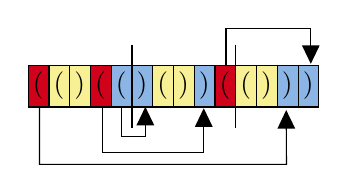
\begin{tikzpicture}[x=0.75pt,y=0.75pt,yscale=-1,xscale=1]
	\draw  [fill={rgb, 255:red, 208; green, 2; blue, 27 }  ,fill opacity=1 ] (160,170) -- (170,170) -- (170,190) -- (160,190) -- cycle;
	\draw  [fill={rgb, 255:red, 247; green, 240; blue, 148 }  ,fill opacity=1 ] (170,170) -- (180,170) -- (180,190) -- (170,190) -- cycle;
	\draw  [fill={rgb, 255:red, 247; green, 240; blue, 148 }  ,fill opacity=1 ] (180,170) -- (190,170) -- (190,190) -- (180,190) -- cycle;
	\draw  [fill={rgb, 255:red, 208; green, 2; blue, 27 }  ,fill opacity=1 ] (190,170) -- (200,170) -- (200,190) -- (190,190) -- cycle;
	\draw  [fill={rgb, 255:red, 139; green, 181; blue, 229 }  ,fill opacity=1 ] (200,170) -- (210,170) -- (210,190) -- (200,190) -- cycle;
	\draw  [fill={rgb, 255:red, 139; green, 181; blue, 229 }  ,fill opacity=1 ] (210,170) -- (220,170) -- (220,190) -- (210,190) -- cycle;
	\draw  [fill={rgb, 255:red, 247; green, 240; blue, 148 }  ,fill opacity=1 ] (220,170) -- (230,170) -- (230,190) -- (220,190) -- cycle;
	\draw  [fill={rgb, 255:red, 247; green, 240; blue, 148 }  ,fill opacity=1 ] (230,170) -- (240,170) -- (240,190) -- (230,190) -- cycle;
	\draw  [fill={rgb, 255:red, 139; green, 181; blue, 229 }  ,fill opacity=1 ] (240,170) -- (250,170) -- (250,190) -- (240,190) -- cycle;
	\draw  [fill={rgb, 255:red, 208; green, 2; blue, 27 }  ,fill opacity=1 ] (250,170) -- (260,170) -- (260,190) -- (250,190) -- cycle;
	\draw  [fill={rgb, 255:red, 247; green, 240; blue, 148 }  ,fill opacity=1 ] (260,170) -- (270,170) -- (270,190) -- (260,190) -- cycle;
	\draw  [fill={rgb, 255:red, 247; green, 240; blue, 148 }  ,fill opacity=1 ] (270,170) -- (280,170) -- (280,190) -- (270,190) -- cycle;
	\draw  [fill={rgb, 255:red, 139; green, 181; blue, 229 }  ,fill opacity=1 ] (280,170) -- (290,170) -- (290,190) -- (280,190) -- cycle;
	\draw  [fill={rgb, 255:red, 139; green, 181; blue, 229 }  ,fill opacity=1 ] (290,170) -- (300,170) -- (300,190) -- (290,190) -- cycle;
	\draw    (210,160) -- (210,200);
	\draw    (260,160) -- (260,200);
	\draw    (205.14,190.29) -- (205.14,204.36) -- (216.43,204.36) -- (216.43,192.93);
	\draw [shift={(216.43,189.93)}, rotate = 90] [fill={rgb, 255:red, 0; green, 0; blue, 0 }  ][line width=0.08]  [draw opacity=0] (8.93,-4.29) -- (0,0) -- (8.93,4.29) -- cycle;
	\draw    (195.57,189.79) -- (195.57,212.07) -- (244.57,212.07) -- (244.57,193.64);
	\draw [shift={(244.57,190.64)}, rotate = 90] [fill={rgb, 255:red, 0; green, 0; blue, 0 }  ][line width=0.08]  [draw opacity=0] (8.93,-4.29) -- (0,0) -- (8.93,4.29) -- cycle;
	\draw    (165.43,190.21) -- (165.43,217.64) -- (284.43,217.64) -- (284.3,194.5);
	\draw [shift={(284.29,191.5)}, rotate = 89.69] [fill={rgb, 255:red, 0; green, 0; blue, 0 }  ][line width=0.08]  [draw opacity=0] (8.93,-4.29) -- (0,0) -- (8.93,4.29) -- cycle;
	\draw    (255.29,170.21) -- (255.29,152.07) -- (296.14,152.07) -- (296.14,166.21);
	\draw [shift={(296.14,169.21)}, rotate = 270] [fill={rgb, 255:red, 0; green, 0; blue, 0 }  ][line width=0.08]  [draw opacity=0] (8.93,-4.29) -- (0,0) -- (8.93,4.29) -- cycle;

	\draw (161,172) node [anchor=north west][inner sep=0.75pt]   [align=left] {(};
	\draw (171,172) node [anchor=north west][inner sep=0.75pt]   [align=left] {(};
	\draw (181,172) node [anchor=north west][inner sep=0.75pt]   [align=left] {)};
	\draw (211,172) node [anchor=north west][inner sep=0.75pt]   [align=left] {)};
	\draw (201,172) node [anchor=north west][inner sep=0.75pt]   [align=left] {(};
	\draw (191,172) node [anchor=north west][inner sep=0.75pt]   [align=left] {(};
	\draw (271,172) node [anchor=north west][inner sep=0.75pt]   [align=left] {)};
	\draw (261,172) node [anchor=north west][inner sep=0.75pt]   [align=left] {(};
	\draw (251,172) node [anchor=north west][inner sep=0.75pt]   [align=left] {(};
	\draw (241,172) node [anchor=north west][inner sep=0.75pt]   [align=left] {)};
	\draw (231,172) node [anchor=north west][inner sep=0.75pt]   [align=left] {)};
	\draw (221,172) node [anchor=north west][inner sep=0.75pt]   [align=left] {(};
	\draw (291,172) node [anchor=north west][inner sep=0.75pt]   [align=left] {)};
	\draw (281,172) node [anchor=north west][inner sep=0.75pt]   [align=left] {)};
\end{tikzpicture}

	\caption{Divisione in blocchi di una parola di Dyck.}
	\label{fig:paren_blocks}
\end{figure}

\begin{lemma}[delle incrociate]\label{lem:dyckincro}
	In una parola di Dyck $w$, sia $p$ la posizione di una parentesi aperta. Allora
	\begin{equation*}
		\nexists q\mid p<q<\dyfindclosed(p) \quad\land\quad \dyfindclosed(q)>\dyfindclosed(p)
	\end{equation*}
\end{lemma}
\begin{proof}
	Se $p<q<\dyfindclosed(p)$ allora $E_w(q)>E_w(p)$. Poiché la funzione di eccesso non può scendere sotto il valore $E_w(q)$ senza raggiungere $\dyfindclosed(q)$, è impossibile che valga $\dyfindclosed(q)>\dyfindclosed(p)$.
\end{proof}

\noindent La struttura si compone di diverse componenti:
\begin{itemize}
	\item la parola $w$ memorizzata come sequenza di bit (un valore booleano per le parentesi aperte e l'altro per le chiuse).
	\item un vettore $E$ di $k$ elementi, contenente per ogni blocco il valore della funzione di eccesso nella sua prima posizione;
	\item un vettore $M$ che contiene, per ogni pioniera o relativa chiusa, l'indice della sua corrispondente;
	\item un vettore $O$ di $k$ elementi, contenente per ogni blocco l'ultima posizione prima di esso in cui la funzione di eccesso è minore del minimo in tale blocco;
	\item un vettore $\bar p$ di bit che identifica a $1$ le pioniere, a cui è associata una struttura succinta di rango e selezione;
\end{itemize}

\subsubsection{Implementazione dell'interfaccia}
\newcommand{\dyfindopenb}{\mathbf{find\_open}}
\newcommand{\dyfindclosedb}{\mathbf{find\_closed}}
\newcommand{\dyencloseb}{\mathbf{enclose}}
Per semplicità ci riferiremo con abuso di notazione ai simboli e alle rispettive posizioni intercambiabilmente.

\paragraph{$\dyfindclosedb$} È data la posizione $p$ di un'aperta. Sia $B=\floor{p/k}$ il blocco a cui $p$ appartiene.
L'algoritmo si compone dei seguenti passi:
\begin{enumerate}
	\item \label{en:dyfc:1} a partire da $E[B]$, ricavare l'eccesso $E_w(p)$ calcolando e salvando quello di ogni simbolo del blocco fino a $p$;
	\item calcolando gli eccessi delle posizioni successive a $p$ nel blocco, determinare se $p$ è vicina.
	      È così se e solo se esiste una posizione $r\neq p$ tale che $E_w(r)=E_w(p)$. Se si trova un tale $r$, restituire $r$; altrimenti $p$ è lontana;
	\item se $p$ è lontana allora si chiude in un blocco $B'\neq B$.
	      Se $\bar p[p]=1$ allora $p$ è una pioniera, precisamente la $(\rank_{\bar p}(p)+1)$-esima, quindi la chiusa corrispondente si trova in $M[\rank_{\bar p}(p)+1]$ e va restituito tale valore;
	\item se $\bar p_p=0$ allora $p$ non è una pioniera.
	      La pioniera precedente a $p$, ovvero la $(\rank_{\bar p}(p))$-esima, è la pioniera di riferimento di $p$, ossia è la pioniera in posizione $q=\select_{\bar p}(\rank_{\bar p}(p)-1)$ che si chiude nel blocco $B'$.
	      Se così non fosse si contraddirebbe il lemma \ref{lem:dyckincro} delle incrociate. Per lo stesso motivo la pioniera in posizione $q$ è aperta.
	      A partire dalla corrispondente chiusa $q'$ di $q$, in posizione $M[q]$, cercare verso sinistra a partire dalla posizione $q'$ la prima che ha eccesso $E_w(p)$.
	      L'eccesso di $q'$ è lo stesso di $q$, calcolato al passo \ref{en:dyfc:1}.
\end{enumerate}

\paragraph{$\dyfindopenb$} È data la posizione $p$ di una chiusa. Sia $B$ il blocco a cui $p$ appartiene.
L'algoritmo si compone dei seguenti passi:
\begin{enumerate}
	\item a partire da $E[B]$, ricavare l'eccesso $E_w(p)$ calcolando e salvando quello di ogni simbolo del blocco fino a $p$;
	\item se esistono posizioni tra quelle già analizzate con eccesso uguale a $E_w(p)$, restituire l'ultima: $p$ è vicina;
	\item dato che $p$ è lontana, se $\bar p[p]=1$ allora la parentesi in $p$ è una pioniera, precisamente la $(\rank_{\bar p}(p)+1)$-esima, quindi la chiusa corrispondente si trova in $M[\rank_{\bar p}(p)+1]$ e va restituito tale valore;
	\item se $\bar p_p=0$ allora $p$ non è una pioniera.
	      La pioniera successiva a $p$, è la $(\rank_{\bar p}(p)+1)$-esima, in posizione $q=\select_{\bar p}(\rank_{\bar p}(p))$.
	      Calcolare l'eccesso di $q$ procedendo verso destra a partire da $p$.
	      A partire dalla corrispondente aperta $q'$ di $q$, in posizione $M[q]$ e che ha lo stesso eccesso di $q$, cercare verso destra a partire dalla posizione $q'$ la prima che ha eccesso $E_w(p)$ e restituire il valore.
\end{enumerate}

\paragraph{$\dyencloseb$} È data una posizione $x$ in input.
Se $x$ è la posizione di un'aperta, sia $p:=x$ e $p':=\dyfindclosed_w(x)$, altrimenti sia $p=\dyfindopen_w(x)$ e $p'=x$.
Sia $B$ il blocco a cui $p$ appartiene.
L'algoritmo si compone dei seguenti passi:
\begin{enumerate}
	\item a partire da $E[B]$, ricavare l'eccesso $E_w(p)$, facendo in modo di mantenere in memoria l'ultima posizione $r$, se ne esiste una, per cui $E_w(r)=E_w(p)-1$;
	\item se $r$ esiste, restituire $r$;
	\item \label{en:dyen:3} sia $B'$ il blocco a cui appartiene $p'$ (si noti che non necessariamente $B'\neq B$).
	      Se esiste in tale blocco una posizione $r>p'$ tale che $E_w(r)=E_w(p')-1=E_w(p)-1$, restituire $\dyfindopen(r)$;
	\item si ha che $p$ ha il minimo eccesso in $B$.
	      Infatti, nelle posizioni minori di $p$ non è stato trovato l'eccesso $E_w(p)-1$, mentre per le posizioni maggiori vale uno dei seguenti casi:
	      \begin{itemize}
		      \item se $B'\neq B$, allora l'eccesso delle posizioni tra $p$ e $p'$ è almeno $E_w(p)$ in quanto ogni parentesi è avvolta da $p$ e $p'$;
		      \item se $B'=B$, allora per le posizioni successive a $p'$ si è visto al passo \ref{en:dyen:3} che non esiste posizione con eccesso uguale a $E_w(p)-1$.
	      \end{itemize}
	      restituire quindi $O[B]$.
\end{enumerate}

\begin{theorem}
	In una parola di Dyck $w$ divisa in $k\geq 2$ blocchi $B_1,\dots,B_k$, esistono $\card{\dypion(w)}\leq 2k-3$ pioniere.
\end{theorem}
% TODO: spostare in appendice?
\begin{proof}
	Per induzione su $k$:
	\begin{itemize}
		\item se $k=2$, si verifica uno e uno solo dei seguenti casi:
		      \begin{itemize}
			      \item nel primo blocco ogni parentesi è vicina, quindi il numero di pioniere è $0$. Quindi $\card{\dypion(w)}=0\leq 2k-3=1$;
			      \item esiste una sola pioniera in quanto ogni lontana in $B_1$ si chiude in $B_2$. Quindi $\card{\dypion(w)}=1\leq 2k-3=1$.
		      \end{itemize}
		\item per ipotesi induttiva, $\card{\dypion(w')}\leq 2k'-3~\forall k'<k,w'$. Si verifica uno e uno solo dei seguenti casi:
		      \begin{enumerate}
			      \item \label{en:dythm:1} se $w$ è debolmente bilanciata, esiste una posizione $p$ nel blocco $B_i$ entro cui tutte le pioniere aperte precedentemente si chiudono.
			            In questo caso, si considerino le parole $w':=w_1\cdots w_p$ e $w'':=w_{p+1}\cdots w_l$, che ereditano i blocchi da $w$ ottenendo $k'$ e $k''$ blocchi ($B_i$ è diviso tra le due ma presente in entrambe, così che $k=k'+k''-1$).
			            Poiché le pioniere di $w$ sono preservate, vale $\card{\dypion(w)}=\card{\dypion(w')}+\card{\dypion(w'')}$.
			            Poiché $w'$, $k'$, $w''$ e $k''$ sono tali da poter applicare l'ipotesi induttiva, vale
			            \begin{align*}
				            \card{\dypion(w)} & = \card{\dypion(w')}+\card{\dypion(w'')} \\
				                              & \leq (2k'-3)+(2k''-3)                    \\
				                              & = 2(k'+k''-3)                            \\
				                              & = 2(k-2) = 2k-4
			            \end{align*}
			      \item Se $w$ è fortemente bilanciata, allora esiste una pioniera che si apre nel primo blocco e si chiude nell'ultimo. Infatti, se così non fosse, sia $p$ la pioniera del primo blocco che si chiude nel blocco massimale (più lontano) $B_k$, con $k'<k$. Per il lemma \ref{lem:dyckincro} delle incrociate, le parentesi incluse tra $p$ e la sua chiusa $p'$ non possono chiudersi dopo $p'$. Inoltre la coppia $(p,p')$ non può essere racchiusa da un'altra coppia, altrimenti $p$ non sarebbe la pioniera che si chiude nel blocco massimale. Quindi l'eccesso in $p'$ è $0$, il che è assurdo.

			            Sia $p$ la prima pioniera di $w$. Si possono rimuovere coppie di parentesi che precedono $p$ o seguono la sua chiusa in quanto sono vicine e non contribuiscono al numero di pioniere. Si può inoltre rimuovere la parentesi $p$ e la relativa chiusa ottenendo una parola risultante $w'$ ancora bilanciata. Per $w'$ vale uno e uno solo dei seguenti casi:
			            \begin{itemize}
				            \item se si rimuove un intero blocco, ossia $k'<k$, si ha rimosso una pioniera. Per ipotesi induttiva $\dypion(w)=\dypion(w')+1\leq 2k'-3+1\leq 2k-4\leq 2k-3$;
				            \item se $w'$ è debolmente bilanciata, si ha rimosso una pioniera e si ricade nel caso \ref{en:dythm:1}. Quindi $\dypion(w)=\dypion(w')+1\leq 2k-4+1\leq 2k-3$;
				            \item se $w'$ è ancora fortemente bilanciata, selezionare una nuova pioniera $p'$ e ripetere il procedimento di rimozione appena descritto. Il numero di pioniere non cambia tra $w$ e $w'$.
			            \end{itemize}
		      \end{enumerate}
	\end{itemize}
\end{proof}

Lo spazio occupato in bit da queste strutture è:
\begin{equation*}
	\begin{aligned}
		 & E & k  \log_2(n)         \\
		 & M & \leq 2(2k-3)\log_2 n \\
		 & p & n + o(n)             \\
		 & O & k  \log_2(n)         \\
		 & w & n
	\end{aligned}
\end{equation*}
Se si sceglie $l=\log_2 n$, si fa uso di un totale di al più $D_n=(6k-6)\log_2 n+2n+o(n)=8n+o(n)$ bit. Per confrontare questa grandezza con l'information theoretical lower bound consideriamo due insiemi isomorfi alle parentesi ben bilanciate: le foreste ordinate e gli alberi binari.


\subsection{Information theoretical lower bound}

\subsubsection{Parole di Dyck e foreste ordinate}
$F_n$, con $n\in\N$, è l'insieme delle foreste ordinate con $n$ nodi.
% TODO: essere più formali?
\begin{defin}
	Induttivamente:
	\begin{itemize}
		\item la foresta vuota $\seq{}$ appartiene a $F_0$;
		\item siano $f\in F_n$ e $g\in F_m$. Sia $\tree(f)$ l'albero ottenuto unendo sotto un'unica radice gli alberi di $f$. Allora $\seq{\tree(f),g}\in F_{n+m+1}$.
	\end{itemize}
\end{defin}

\begin{figure}[ht]
	\centering
	\begin{tikzpicture}[scale=0.8]
	\node[int] (T0) {} child { node[leaf] {}};

	\node[int,right=1.5cm of T0] (T1) {}
	child {node[leaf] {} }
	child {node[leaf] {} };

	\node[int,right=2.5cm of T1] (T1) {}
	child {node[int] {}
			child {node[leaf] {}}
		}
	child {node[leaf] {} }
	child {node[int] {}
			child {node[leaf] {}}
			child {node[leaf] {}}
		};
\end{tikzpicture}

	\caption{Foresta ordinata.}
	\label{fig:ordered_forest}
\end{figure}

Si consideri la funzione $\varphi:D_n\to F_n$, definita induttivamente come segue:
\begin{itemize}
	\item $\varphi(\emptyword)=\seq{}$;
	      % TODO: questa notazione è tecnicamente sbagliata in quanto ogni foresta sarebbe una coppia albero-foresta. Pensare a una notazione migliore
	\item $\varphi(~(w_1)w_2~)=\seq{\tree(\varphi(w_1)),\varphi(w_2)}$.
\end{itemize}

Come si può facilmente verificare la funzione descritta è biiettiva, in quanto una foresta ordinata appartiene a una e una sola delle forme delle immagini di $\varphi$.


\subsubsection{Foreste ordinate e alberi binari}
Si consideri la funzione $B:F_n\to B_n$ (dove $B_n$ è l'insieme degli alberi binari con $n$ nodi interni), definita induttivamente come segue:
% TODO: anche qui si potrebbe essere più formali. Per rivedere queste definizioni andrebbero riviste quelle di albero binario al relativo paragrafo
\begin{itemize}
	\item $B(\seq{})$ è l'albero costituito dalla sola radice;
	\item $B(\seq{\tree(f)},g)$ è l'albero binario costituito da una radice che ha per figlio sinistro $B(f)$ e destro $B(g)$.
\end{itemize}

\begin{figure}[ht]
	\centering
	% TODO: bruttissima, migliorare
	\begin{tikzpicture}[recurse/.style={rectangle,draw},scale=0.8]
	\node (T0) {$B\left(\left\langle\tikz\node[int,scale=0.6] {};, \raisebox{-2mm}{\tikz[scale=0.3,every node/.style={scale=0.6}] \node[int] {} child {node[leaf] {}};}\,\right\rangle\right)\,=$ };

	\node (T1) [above right=3mm and 13mm of T0,int] {}
	child[sibling distance=18mm] {node[recurse] {$B(\seq{})$} }
	child[sibling distance=18mm] {node[recurse] {$B\left(\left\langle\,\raisebox{-2mm}{\tikz[scale=0.3,every node/.style={scale=0.6}] \node[int] {} child {node[leaf] {}};}\,\right\rangle\right)$} };
	\node[right=31mm of T0] (u1) {$=$};

	\node (T2) [above right=3 mm and 29mm of T1,int] {}
	child {node[leaf] {} }
	child {node[int] {}
			child {node[recurse] {$B(\seq{\tikz\node[int,scale=0.6] {};})$}}
			child {node[recurse] {$B(\seq{})$}}
		};
	\node[right=24mm of u1] (u2) {$=$};

	\node (T3) [above right=2mm and 32mm of T2,int] {}
	child {node[leaf] {} }
	child {node[int] {}
			child {node[int] {}
					child {node[recurse] {$B(\seq{})$} }
					child {node[recurse] {$B(\seq{})$} }
				}
			child {node[leaf] {} }
		};
	\node[right=27mm of u2] {$=$};

	\node (T4) [right=2.7cm of T3,int] {}
	child {node[leaf] {} }
	child {node[int] {}
			child {node[int] {}
					child {node[leaf] {} }
					child {node[leaf] {} }
				}
			child {node[leaf] {} }
		};
\end{tikzpicture}

	\caption{Esempio di calcolo isomorfismo tra foreste e alberi binari.}
	\label{fig:iso_forest_bintree_example}
\end{figure}

Dal momento che i tre insiemi sono isomorfi, le loro cardinalità sono uguali. Come visto al \cref{thm:catalano}:
\begin{equation*}
	\card{D_n}=\card{F_n}=\card{B_n}=C_n \text,
\end{equation*}
da cui
\begin{equation*}
	Z_n=\log_2(C_n)=O(n) \text{ bit}.
\end{equation*}
Ergo, la struttura vista per l'ADT delle parentesi ben bilanciate che ha un costo in spazio di $8n+o(n)$ bit è compatta.



\section{Tecniche di hashing}
Una funzione di hash $h:U\to n$ associa ogni elemento di un universo $U$ a un numero da $0$ a $n-1$, detto bucket.

Se $U$ è finito, il numero di funzioni di hash con $n$ bucket su universo $U$ è $n^{|U|}$.

L'analisi che segue si basa su alcune assunzioni, solo approssimabili nella pratica\footnote{
	In genere, se $\Sigma$ è un alfabeto e $U=\Sigma^{\leq l}$, una funzione di hash $h: U\to n$ viene memorizzata tramite valori casuali $w=\angle{l_i}_{i\in l}$ inclusi tra $0$ e $\card\Sigma-1$ e calcolata come $h(s)=\left(\sum_{i=0}^{l-1} s_i w_i\right) \mod n$. Tipicamente vengono imposti vincoli su $n$ (ad esempio che sia primo). È facile vedere che questa tecnica non rispetta le condizioni.
}:
\begin{itemize}
	\item $h$ è calcolabile in tempo costante rispetto a $\card U$;
	\item $h$ occupa spazio costante rispetto a $\card U$;
	\item fissati $U$ e $n$ è possibile estrarre uniformemente a caso una funzione di hash $h:U\to n$ (\flang{full randomness assumption}).
\end{itemize}


\subsection{Sequenze di peeling di un grafo}
Le sequenze di peeling di un grafo generalizzano la nozione di aciclicità agli ipergrafi e forniscono una tecnica applicabile al metodo MWHC.

\begin{defin}
	Sia $G=(V,E)$ un grafo non orientato. Una sequenza di peeling per $G$ è una sequenza di coppie $\tuple{e_i,x_i}\in E\times V$, con $x_i\in e_i$, in cui appaiono tutti i lati e tale per cui nessun vertice $x_i$ (detto cardine o \flang{hinge}) è apparso nei lati $i$.
\end{defin}

\begin{figure}[ht]
	\begin{center}
		% TODO: pessimo esempio, migliorare
		\begin{subfigure}[b]{0.45\textwidth}
			\begin{center}
				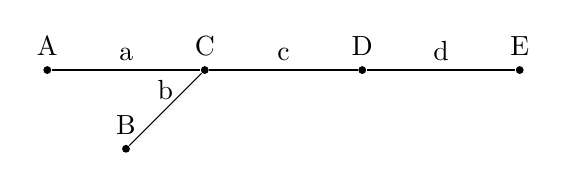
\begin{tikzpicture}
	\node [circle,fill,label=above:{A},inner sep=1pt](A) at (0,0) {};
	\node [circle,fill,label=above:{B},inner sep=1pt](B) at (1,-1) {};
	\node [circle,fill,label=above:{C},inner sep=1pt](C) at (2,0) {};
	\node [circle,fill,label=above:{D},inner sep=1pt](D) at (4,0) {};
	\node [circle,fill,label=above:{E},inner sep=1pt](E) at (6,0) {};

	\draw (A) -- (C) node [midway,above] {a};
	\draw (B) -- (C) node [midway,above] {b};
	\draw (C) -- (D) node [midway,above] {c};
	\draw (D) -- (E) node [midway,above] {d};
\end{tikzpicture}

			\end{center}
		\end{subfigure}
		\begin{subfigure}[b]{0.45\textwidth}
			\begin{center}
				\begin{align*}
					a & = \{(A, C), A\} \\
					b & = \{(B, C), B\} \\
					c & = \{(C, D), D\} \\
					d & = \{(D, E), E\}
				\end{align*}
			\end{center}
		\end{subfigure}
	\end{center}
	\caption{Un grafo e una sequenza di peeling valida.}%
	\label{fig:example_peeling}
\end{figure}

Il risultato fondamentale sulle sequenze di peeling lega la loro presenza a quella di cicli:
\begin{theorem}
	Un grafo ammette una sequenza di peeling se e solo se è aciclico.
\end{theorem}

\subsubsection{Sequenze di peeling di un ipergrafo}
Un $r$-ipergrafo uniforme $G=(V,E)$ è composto da un insieme $V$ di vertici e uno $E$ di iperlati, dove ogni iperlato è un insieme di $r$ vertici\footnote{Negli $r$-ipergrafi generici un iperlato ha al più $r$ vertici.} (i.e. $E\subseteq\binom{V}{r}$).

Le sequenze di peeling si definiscono sugli ipergrafi in modo del tutto analogo a quello per i grafi, come un insieme di coppie iperlato-cardine. Per definizione, un ipergrafo è aciclico se e solo se ammette una sequenza di peeling.



\subsection{La tecnica MWHC}
La tecnica MWHC\footnote{Da Majewski Wormald Havas Czech \cite{Majewski:96:MWHC}} ha lo scopo di memorizzare un dizionario statico (ossia immutabile).
Si consideri un insieme universo $U$ e un insieme $S\subset U$ di chiavi tale che $m:=\card S\ll\card U$. Si fissi inoltre una costante $r\in\N^+$.
Un dizionario $D$ ha in input un valore $x\in U$ e produce un output.
È data una funzione $f:S\to 2^r$ detta \emph{prescritta}: l'output di $D$ è $f(x)$ se $x\in S$, mentre può consistere in qualunque valore se $x\in U\setminus S$.

La tecnica HWHC permette di ricavare la prescritta in una data chiave senza la necessità di memorizzare alcuna chiave. Per fare ciò, vengono estratte casualmente due funzioni di hash $h_1,h_2:U\to n$.
Viene poi costruito un grafo non orientato $G=(V,E)$, dove $V=n$ e $E=\set{\set{h_1(x),h_2(x)}\mid x\in S}$ (quindi $\card E=m$).
Se si verifica una delle seguenti condizioni, l'estrazione di $h_1$ e $h_2$ viene ripetuta:
\begin{itemize}
	\item $\exists x,y\mid \set{h_1(x),h_2(x)}=\set{h_1(y)=h_2(y)}$;
	\item $\exists x\mid h_1(x)=h_2(x)$;
	\item $G$ contiene cicli.
\end{itemize}

Per poter calcolare i valori di $f$ senza doverli memorizzare, si costruisce un sistema di $m$ equazioni, una per ogni $x\in S$, del tipo
\begin{equation*}
	(w_{h_1(x)} + w_{h_2(x)}) \mod 2^r = f(x) \text,
\end{equation*}
dove $w_0,\dots,w_{n-1}$ sono variabili.

Poiché $G$ è aciclico esiste per esso una sequenza di peeling. Ordinando le equazioni come la sequenza (gli indici delle variabili corrispondenti agli elementi di ciascun arco) e risolvendo ciascuna equazione nel suo cardine, si può portare il sistema in una forma risolvibile trivialmente ("a gradini").

Memorizzate le soluzioni $w_i$ del sistema in un vettore $W$, si può calcolare $f(x)$ per un dato $x\in S$ con la formula
\begin{equation*}
	f(x) = (W[h_1(x)] + W[h_2(x)]) \mod 2^r
\end{equation*}

% TODO: necessario un esempio

Per quanto riguarda il dimensionamento di $n$, se $n\leq m$ allora il grafo è necessariamente ciclico ed è impossibile quindi determinare le funzioni di hash.
Per $n>m$, \cite{Majewski:96:MWHC} dimostra:
\begin{theorem}
	Se $n>2.09m$, la procedura di selezione di $h_1$ e $h_2$ termina in un numero atteso di $2$ tentativi.
\end{theorem}
Adattando la procedura all'utilizzo di un $3$-ipergrafo, il rapporto $\gamma$ tra $n$ e $m$ è minimo: $n>1.23m$.
Il costo in spazio di questa struttura è quello per salvare i valori di $n$ variabili di $r$ bit. Considerato il rapporto tra $n$ e $m$ regolato da $\gamma$, tale costo è di $\gamma rm$ bit. Poiché si sta memorizzando una funzione $f:m\to 2^r$, le cui sono in numero $(2^r)^m$, l'information theoretical lower bound è $rm$ e pertanto, essendo $\gamma$ costante, la struttura è compatta.

\subsubsection{MWHC compresso}
Il sistema della tecnica MWHC è indeterminato, con un numero di gradi di libertà di $n-m$. Ponendo le variabili libere a $0$, e mantenendo i valori non nulli solo per i cardini, si ottiene un vettore $W$ con al più $m$ valori non nulli.
È sufficiente quindi memorizzare $m$ valori per le variabili, sfruttando un array di $\gamma m$ bit, provvisto di struttura di rango, che indichi quali delle variabili totali sono non nulle.

Lo spazio occupato per questa struttura compressa è di $mr+\gamma m+o(m)=O(mr)$ bit, con un numero di bit per chiave di $r+\gamma$, contro i $r\gamma$ della versione non compressa.
Il suo utilizzo è quindi conveniente per $r>\frac{\gamma}{\gamma-1}$ ($r>5$ nel caso di $3$-ipergrafi).


\subsection{Hashing minimale perfetto}
Sia $U$ l'insieme universo e $S\subseteq U$, con $m:=\card S$. Una funzione di hash $H:U\to n$ si dice
\begin{description}
	\item[perfetta] per $S$ se $\forall s_1,s_2\in S:~H(s_1)=H(s_2)\impl s_1=s_2$ (se $H$ è "iniettiva" su $S$);
	\item[minimale] per $S$ se $n=\card S$.
\end{description}

Il problema di determinare una funzione di hashing minimale perfetto (MPHF, \flang{minimal perfect hashing function}) per un dato insieme $S$ viene risolto da una costruzione simile alla precedente. \cite{Majewski:96:MWHC}

Si vuole costruire una funzione $H:U\to m$ minimale e perfetta per $S$.
Questa volta si costruisce un sistema di equazioni del tipo
\begin{equation*}
	(w_{h_0(x)} + w_{h_1(x)} + w_{h_2(x)}) \mod 3 = k \text,
\end{equation*}
dove $k$ è l'indice della funzione di hash che determina il cardine della peeling sequence (i.e., $k=0$ se il cardine dell'iperlato $\set{h_0(x),h_1(x),h_2(x)}$ è $h_0(x)$, etc.).

Come per la tecnica MWHC, si risolve il sistema grazie alla sequenza di peeling e si salvano i valori delle variabili $w$ in un vettore $W$ di $m$ elementi, ciascuno di $2$ bit.
Si definisce poi la funzione $\bar H:U\to n$ calcolata come segue:
\begin{equation*}
	\bar H(x) = h_{(W[h_0(x)] + W[h_1(x)] + W[h_2(x)]) \mod 3}(x)
\end{equation*}
La funzione restituisce il valore del cardine dell'arco identificato da $x$, pertanto la funzione è perfetta (ossia, iniettiva su $S$).

La funzione non è, in generale, minimale, in quanto può restituire valori da $0$ a $n-1$.
Per renderla minimale è necessario "compattare" le immagini, nell'insieme $m$.
Per fare ciò, si consideri un vettore $p$ di rango composto da $n$ bit, il bit $i$ posto a $1$ se il vertice $i$ è cardine.
Ottenuta l'immagine $y=\bar H(x)$ di una stringa $x$, il rango di $y$ in tale vettore fornisce la suddetta compattazione, in quanto consiste nel numero di cardini minori di $i$.
Si ottiene quindi una funzione $H:U\to m$ minimale perfetta per $S$:
\begin{equation*}
	H(x) = \rank_p(\bar H(x))
	= \rank_p(h_{(W[h_0(x)] + W[h_1(x)] + W[h_2(x)]) \mod 3}(x))
\end{equation*}

Il costo spaziale dei due vettori $W$ e $p$ è di $2n+n=3n$ bit.
Per risparmiare $m$ bit, si consideri che dei quattro valori possibili per ciascun elemento di $W$ vengono usati solo tre valori.
Assegnando il valore $3$ agli elementi cardine a $0$, si lascia invariato l'output di $\bar H$ (per via del modulo $3$), ma si può effettuare l'operazione rango direttamente nel vettore $W$, poiché tutti e soli gli elementi diversi da $0$ sono cardini.
Il costo complessivo in bit è quindi di $2n$, ovvero di $2.46m$ se $\gamma=1.23$.

\cleardoublepage

\appendix
\chapter{Laboratorio 1: Cammini disgiunti tramite algoritmo basato su pricing}


\begin{minted}[mathescape, fontsize=\small, xleftmargin=0.5em]{python}
import networkx as nx
import math
from networkx.algorithms.shortest_paths.weighted import dijkstra_path
\end{minted}


Definiamo una funzione per generare grafi in una  forma precisa, ossia a 
\textit{doppio ventaglio}: 

\begin{minted}[mathescape, fontsize=\small, xleftmargin=0.5em]{python}
def doubleFan(k):
    G = nx.DiGraph()
    G.add_nodes_from(['s', 't', 'x', 'y'])
    G.add_nodes_from(['a' + str(i) for i in range(k)])
    G.add_nodes_from(['b' + str(i) for i in range(k)])
    G.add_edges_from([('s', 'a' + str(i)) for i in range(k)])
    G.add_edges_from([('a' + str(i), 'x') for i in range(k)])
    G.add_edges_from([('y', 'b' + str(i)) for i in range(k)])
    G.add_edges_from([('b' + str(i), 't') for i in range(k)])
    G.add_edge('x', 'y')
    return G
\end{minted}

\begin{minted}[mathescape, fontsize=\small, xleftmargin=0.5em]{python}
nx.draw(doubleFan(2))
\end{minted}
\includegraphics[width=0.3 \linewidth]{labs/figures/lab1_figure3_1.pdf}


\begin{minted}[mathescape, fontsize=\small, xleftmargin=0.5em]{python}
nx.draw(doubleFan(4))
\end{minted}
\includegraphics[width=0.3 \linewidth]{labs/figures/lab1_figure4_1.pdf}



\begin{minted}[mathescape, fontsize=\small, xleftmargin=0.5em]{python}
nx.draw(doubleFan(8))
\end{minted}
\includegraphics[width=0.3 \linewidth]{labs/figures/lab1_figure5_1.pdf}


Definiamo, quindi, una funzione che implementa \textsc{PricedDisjointPaths}: 


\begin{minted}[mathescape, fontsize=\small, xleftmargin=0.5em]{python}
def greedyDisjointPaths(G_original, sourceTargetPairs, c = 1):
    G = G_original.copy()
    result = []
    beta = math.pow(G.number_of_edges(), 1 / (c + 1))
    # Set all lengths to 1 and all congestion to 0
    for u,v,d in G.edges(data = True):
        d['length'] = 1
        d['congestion'] = 0
    # Main cycle
    while True:
        minPath = None
        for pairIndex in range(len(sourceTargetPairs)):
            try:
                source = sourceTargetPairs[pairIndex][0]
                target = sourceTargetPairs[pairIndex][1]
                path = dijkstra_path(G, source, target, 'length')
            except:
                pass
            else:
                pathLength = 0
                for i in range(len(path) - 1):
                    pathLength += G[path[i]][path[i+1]]['length']
                if minPath == None or pathLength < minPathLength:
                    minPath = path
                    minPathLength = pathLength
                    minPathIndex = pairIndex
        if minPath == None:
            break
        result.append(minPath)
        sourceTargetPairs.pop(minPathIndex)
        for i in range(len(path) - 1):
            x1 = path[i]
            x2 = path[i+1]
            G[x1][x2]['length'] *= beta
            G[x1][x2]['congestion'] += 1
            if G[x1][x2]['congestion'] == c:
                G.remove_edge(x1, x2)
    return result
\end{minted}



\begin{minted}[mathescape, fontsize=\small, xleftmargin=0.5em]{python}
g = doubleFan(2)
nx.draw(g, with_labels = True)
\end{minted}
\includegraphics[width=0.5 \linewidth]{labs/figures/lab1_figure7_1.pdf}



\begin{minted}[mathescape, fontsize=\small, xleftmargin=0.5em]{python}
greedyDisjointPaths(g, [('s', 't')]*11, c = 10)
\end{minted}
\begin{minted}[fontsize=\small, xleftmargin=0.5em, mathescape, frame = leftline]{text}
[['s', 'a0', 'x', 'y', 'b0', 't'],
 ['s', 'a1', 'x', 'y', 'b1', 't'],
 ['s', 'a0', 'x', 'y', 'b0', 't'],
 ['s', 'a1', 'x', 'y', 'b1', 't'],
 ['s', 'a0', 'x', 'y', 'b0', 't'],
 ['s', 'a1', 'x', 'y', 'b1', 't'],
 ['s', 'a0', 'x', 'y', 'b0', 't'],
 ['s', 'a1', 'x', 'y', 'b1', 't'],
 ['s', 'a0', 'x', 'y', 'b0', 't'],
 ['s', 'a1', 'x', 'y', 'b1', 't']]
\end{minted}



\begin{minted}[mathescape, fontsize=\small, xleftmargin=0.5em]{python}
g = doubleFan(4)
nx.draw(g, with_labels = True)
\end{minted}
\includegraphics[width=0.5 \linewidth]{labs/figures/lab1_figure9_1.pdf}



\begin{minted}[mathescape, fontsize=\small, xleftmargin=0.5em]{python}
greedyDisjointPaths(g, [('s', 't')]*11, c = 10)
\end{minted}
\begin{minted}[fontsize=\small, xleftmargin=0.5em, mathescape, frame = leftline]{text}
[['s', 'a0', 'x', 'y', 'b0', 't'],
 ['s', 'a1', 'x', 'y', 'b1', 't'],
 ['s', 'a2', 'x', 'y', 'b2', 't'],
 ['s', 'a3', 'x', 'y', 'b3', 't'],
 ['s', 'a0', 'x', 'y', 'b0', 't'],
 ['s', 'a1', 'x', 'y', 'b1', 't'],
 ['s', 'a2', 'x', 'y', 'b2', 't'],
 ['s', 'a3', 'x', 'y', 'b3', 't'],
 ['s', 'a0', 'x', 'y', 'b0', 't'],
 ['s', 'a1', 'x', 'y', 'b1', 't']]
\end{minted}


\include{labs/lab2}

\backmatter

\printbibliography[heading=bibintoc]

\end{document}
